\chapter{Results: \Hgg}
\label{chap:hgg_results}

\section{Introduction}
This chapter presents the results of the \Hgg analysis, extracted using the statistical inference techniques introduced in the chapter \ref{chap:hgg_stats}. The measurements of Higgs boson production cross sections and couplings are presented in a number of parametrisations, corresponding to different definitions of the parameters, $\mu^{i,\gamma\gamma}$. The simplest of such parametrisations are the signal strength modifiers, which act as global scaling factors either inclusively or per Higgs boson production mode. The results of the signal strength modifier fits are shown in section \ref{sec:results_mu}. Following this, the STXS fits for which the analysis is configured, are shown in section \ref{sec:results_STXS}. To ensure a reasonable sensitivity to the measured parameters, it is necessary to merge groups of STXS bins in the cross section measurements. The results of three different merging schemes with varying degrees of granularity are presented. Finally, section \ref{sec:results_kappa} shows the fits to Higgs boson coupling modifiers in the $\kappa$-framework~\cite{Heinemeyer:2013tqa}.

\section{Signal strengths}\label{sec:results_mu}
The most-constraining fit that can be performed introduces a common signal strength modifier, $\mu$, for all signal processes. This is defined as the ratio of the observed product of the Higgs boson cross section and diphoton branching fraction to the SM expectation, such that a value of one corresponds directly to the SM prediction. The observed test-statistic curve, $q(\mu)$, is shown by the solid line in Figure \ref{fig:likelihood_mu_inclusive}, in addition to the dashed lines representing the $q(\mu)$ curves when groups of nuisance parameters are fixed to their best-fit values. The best-fit value of $\mu$ and the corresponding 68\% confidence intervals are inferred from the curves to be,

\begin{equation*}
  \mu = 1.12 ^{+0.09}_{-0.09} = 1.12 ^{+0.06}_{-0.06}({\rm{th.}}) ^{+0.03}_{-0.03}({\rm{exp.}}) ^{+0.07}_{-0.06}({\rm{stat.}}),
\end{equation*}
\noindent
where the total uncertainty has been decomposed into contributions from theoretical systematic, experimental systematic and statistical uncertainties, using the method described in section \ref{sec:effect_of_nuisance}. As a result of the increased integrated luminosity that comes with using the full run II data, CMS are now approaching the realm of systematics-limited measurements in Higgs boson physics, where the systematic uncertainties are comparable to, if not larger than, the statistical component. The $\pm$9\% total uncertainty represents the current best constraint on inclusive Higgs boson production from a single decay channel at CMS. The compatibility of this fit with the SM prediction is approximately, $p_{\rm{SM}}=17\%$.

\begin{figure}[htb!]
  \centering
  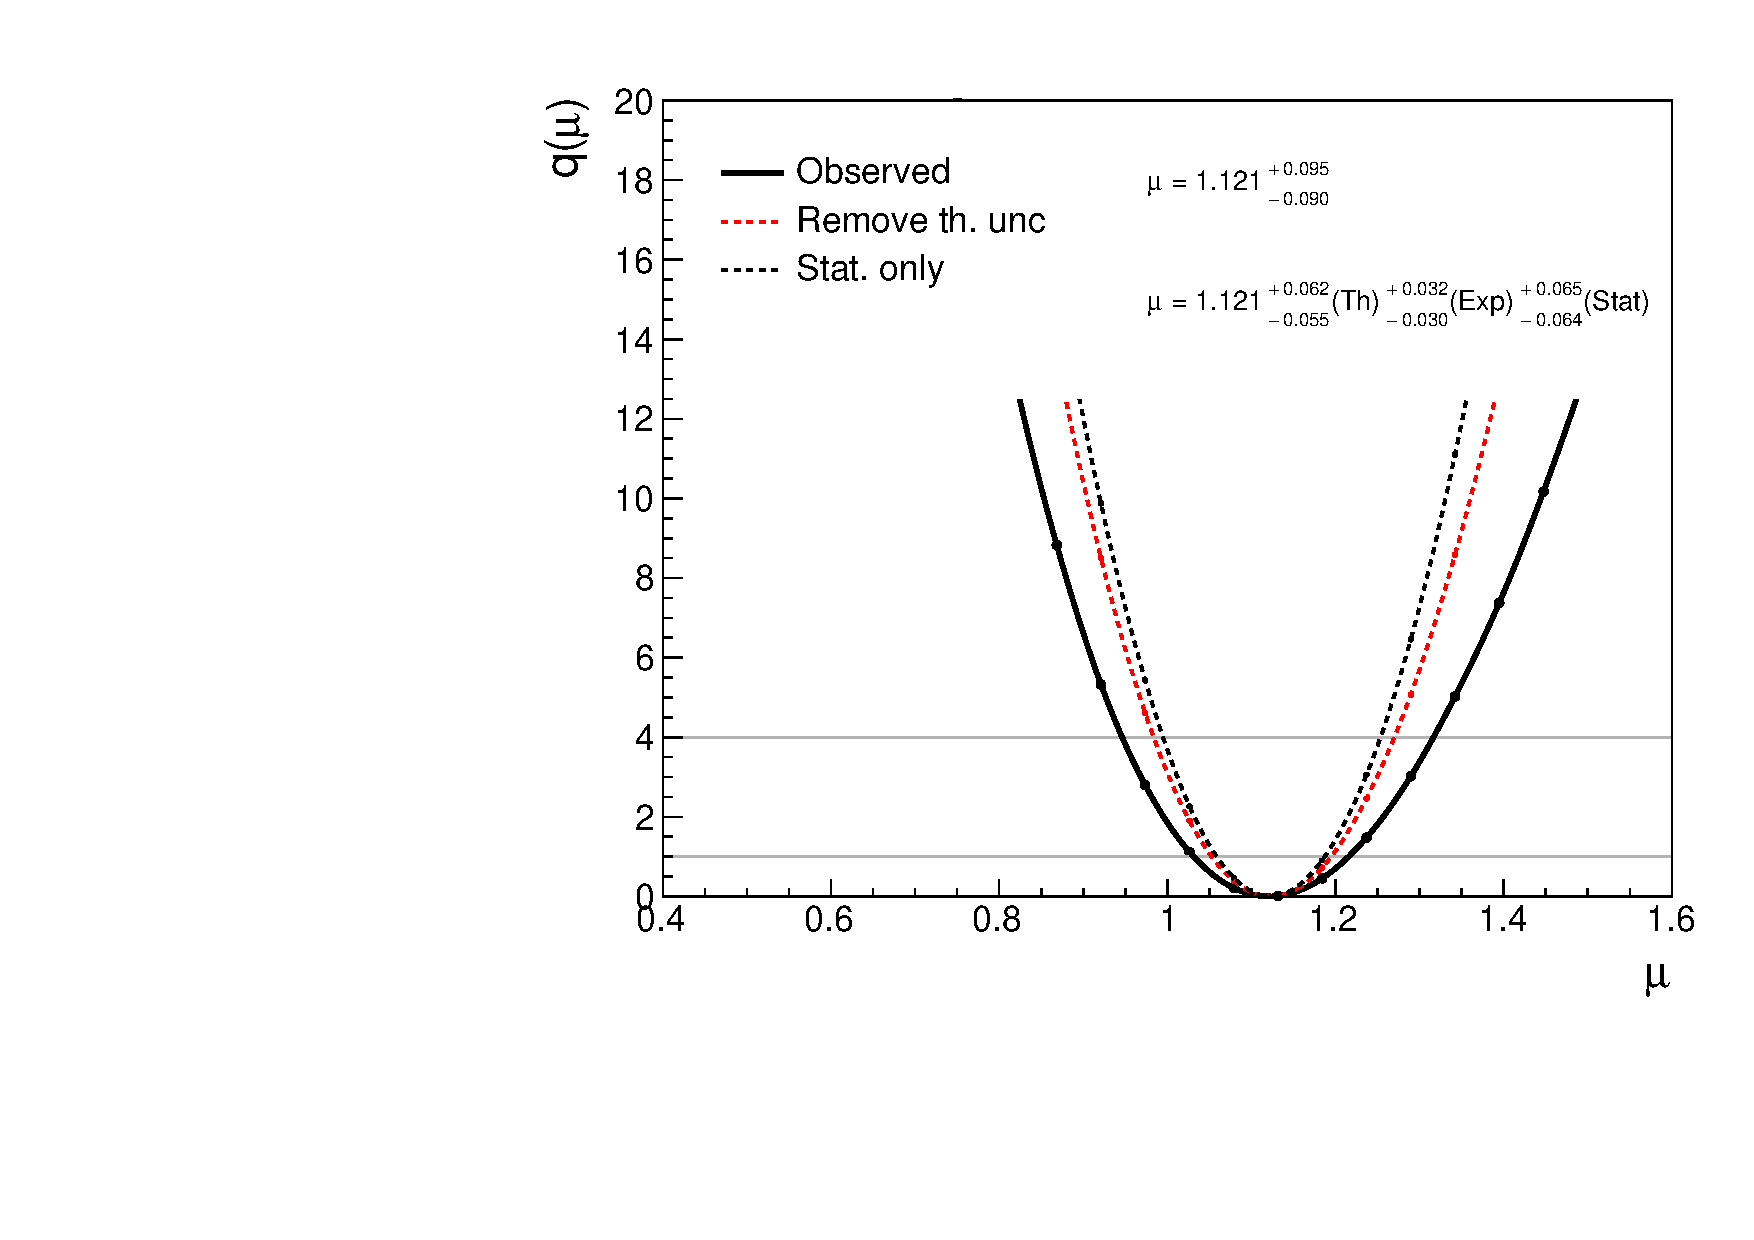
\includegraphics[width=.6\textwidth]{Figures/hgg_results/likelihood_mu.pdf}
  \caption[Observed likelihood curve for the inclusive signal strength]
  {
    Observed likelihood curve as a function of the inclusive signal strength modifier, $\mu$. The likelihood in which all nuisance parameters are profiled is shown by the solid black line. The likelihood curves shown by the dashed lines represent the fits in which all nuisances are fixed to their best fit values in black (stat-only), and only the theoretical uncertainties are fixed to their best-fit values in red.
  }
  \label{fig:likelihood_mu_inclusive}
\end{figure}

The observed diphoton mass distribution in data is shown for the sum of all analysis categories in Figure \ref{fig:sb_inclusive}. In the sum, each category is weighted using the approach detailed in equation \ref{eq:sigmodel_wsum} i.e. weight each category by the ratio of signal to signal-plus-background events, keeping the total absolute signal yield constant. Overlaid, is the best-fit signal-plus-background model obtained in the inclusive signal strength fit. In addition, the uncertainty in the background estimate is shown by the uncertainty bands. These bands are populated by first performing the signal-plus-background fit to data, and then generating many toy data sets from the best-fit background-only model. The green and yellow bands signify the regions in which 68.3\% (1$\sigma$) and 95.4\% (2$\sigma$) of the generated toy data sets lie, respectively. The signal peak is extremely clear above the falling background distribution.

\begin{figure}[htb!]
  \centering
  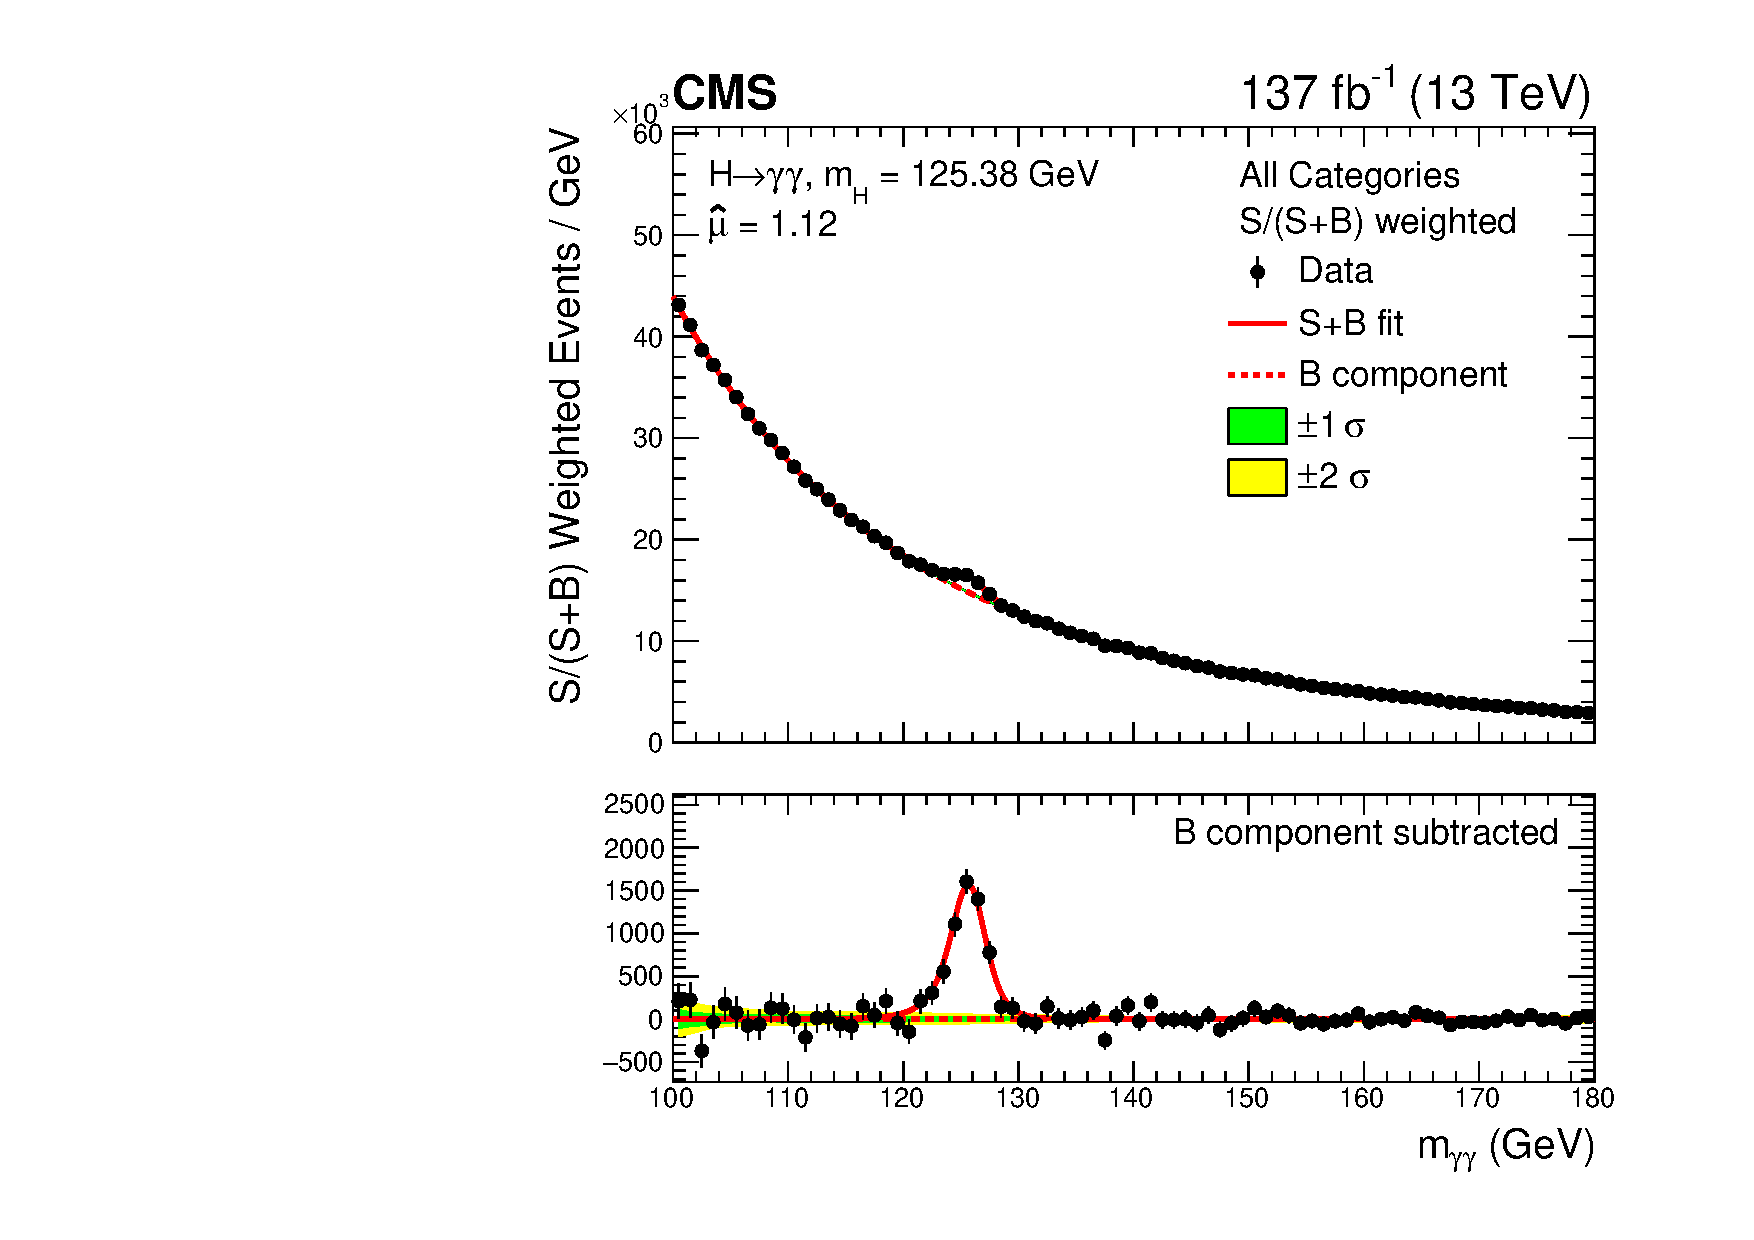
\includegraphics[width=.6\textwidth]{Figures/hgg_results/sPlusBweighted.pdf}
  \caption[Observed diphoton mass distribution for the sum of all analysis categories]
  {
    Data points (black) and the best-fit signal-plus-background model for the sum of all analysis categories is shown. The best-fit model corresponds to the inclusive signal strength fit. In the plot, the events in each category are weighted according to $S_{68}/(S_{68}+B_{68})$, where $S_{68}$ and $B_{68}$ are the expected signal and background estimates, respectively, in a $\pm$1$\sigma_{\rm{eff}}$ window centred on $m_H$, such that the total signal yield remains constant. The solid red line shows the best-fit signal-plus-background model, whereas the dashed line shows the background component only. The one standard deviation (green) and two standard deviation (yellow) bands show the uncertainties in the background component of the fit. The bottom panel shows the residuals after subtraction of this background component.
  }
  \label{fig:sb_inclusive}
\end{figure}

A more granular fit is performed in the signal strength modifier parametrisation, introducing a separate $\mu_i$ parameter for each Higgs boson production mode. Unlike, the subsequent STXS fits described in section \ref{sec:results_STXS}, the VH hadronic and VH leptonic processes are grouped to scale according to $\mu_{\rm{VH}}$, whereas the VBF production mode scales with $\mu_{\rm{VBF}}$. The parameter $\mu_{\rm{top}}$ scales the ttH, tHq, and tHW production modes equally, and $\mu_{\rm{ggH}}$ scales both ggH and bbH production. This defines four independent parameters of interest in total.

The best-fit signal-plus-background model in this signal parametrisation is shown with data in the \mgg distributions in Figure \ref{fig:sb_mu}. Here, the analysis categories have been divided into four groups, corresponding to those targeting the ggH, VBF, VH, and top-associated production modes. In each group, the individual categories are again summed and weighted according to the procedure defined by equation \ref{eq:sigmodel_wsum}. In all cases, the signal peak is clearly visible amongst the smoothly falling background distribution. The equivalent plots for each individual analysis category are presented in Appendix \ref{app:diphoton_mass}.

\begin{figure}[htb!]
  \centering
  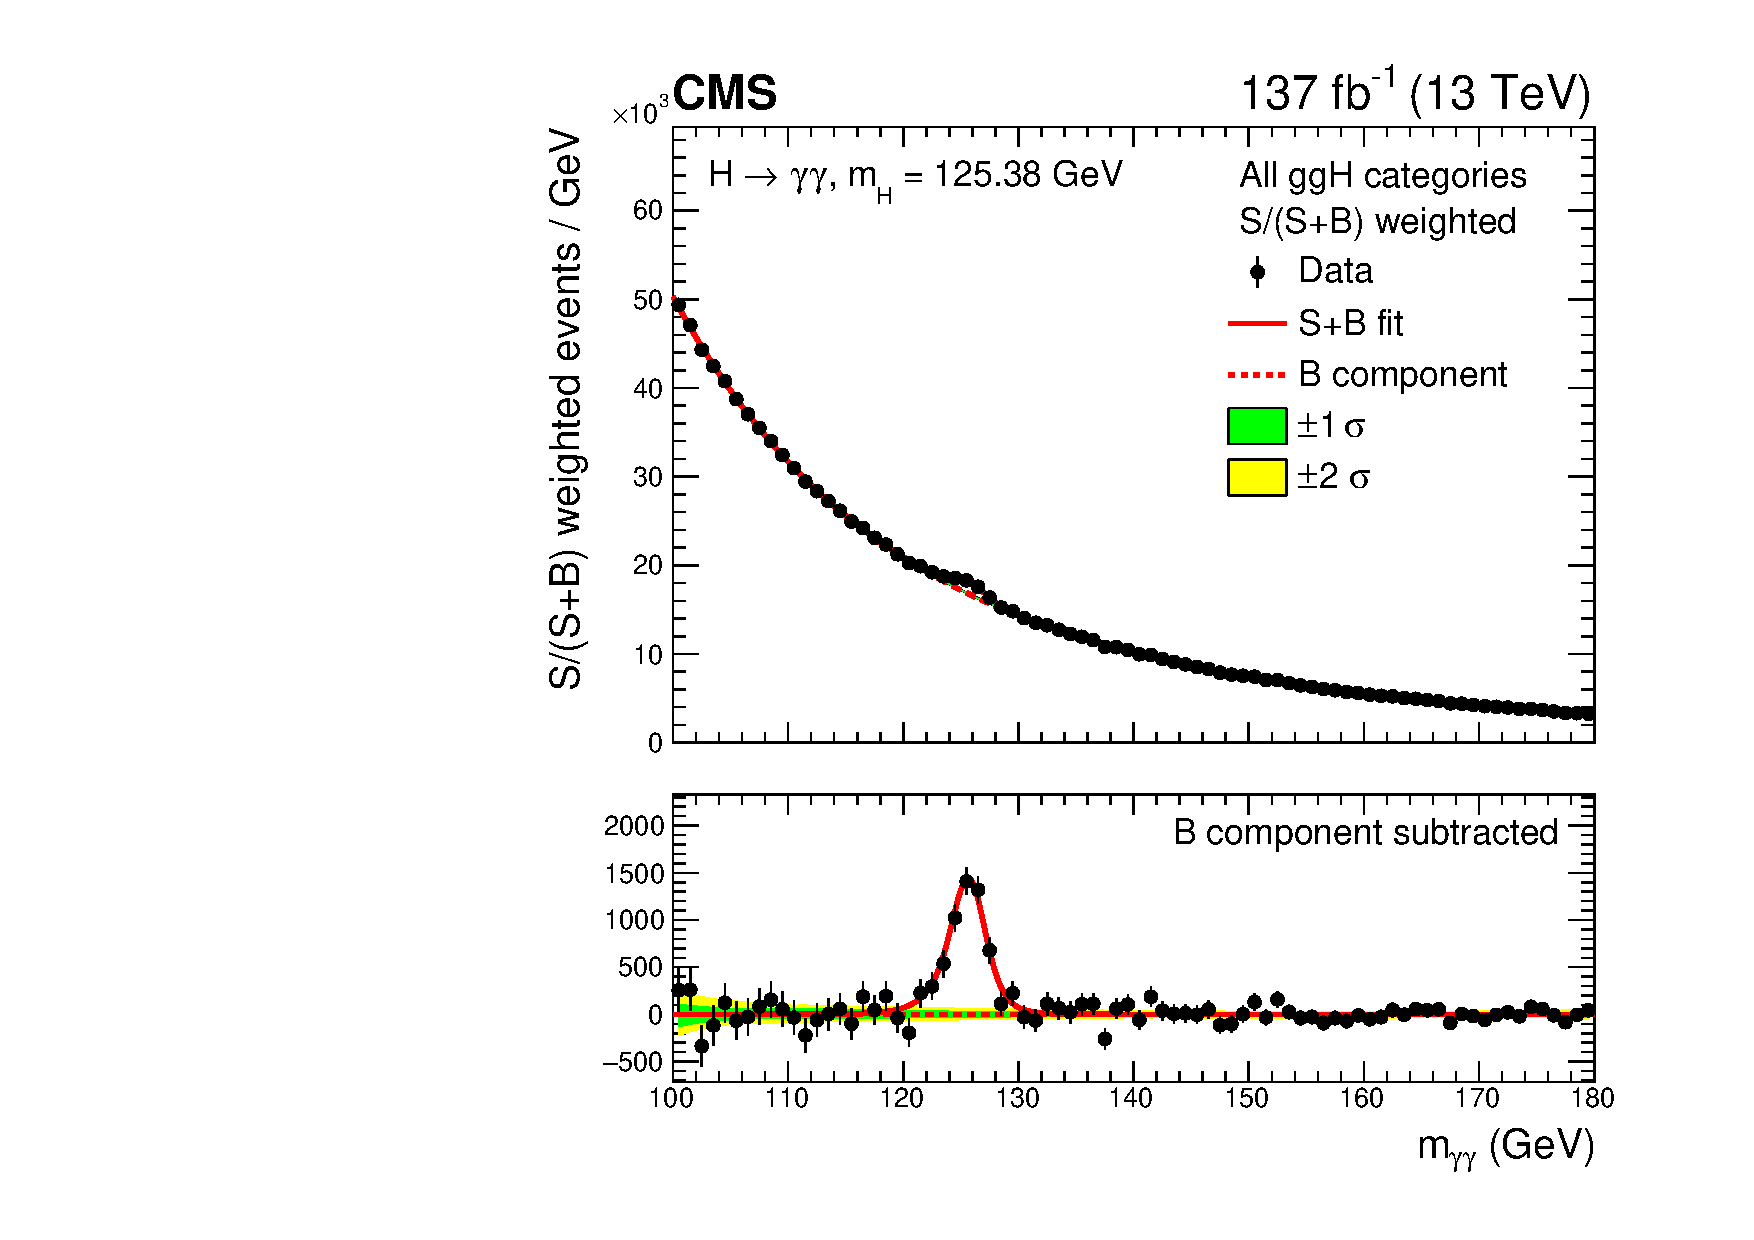
\includegraphics[width=.49\textwidth]{Figures/hgg_results/sPlusBweighted_ggH.pdf}
  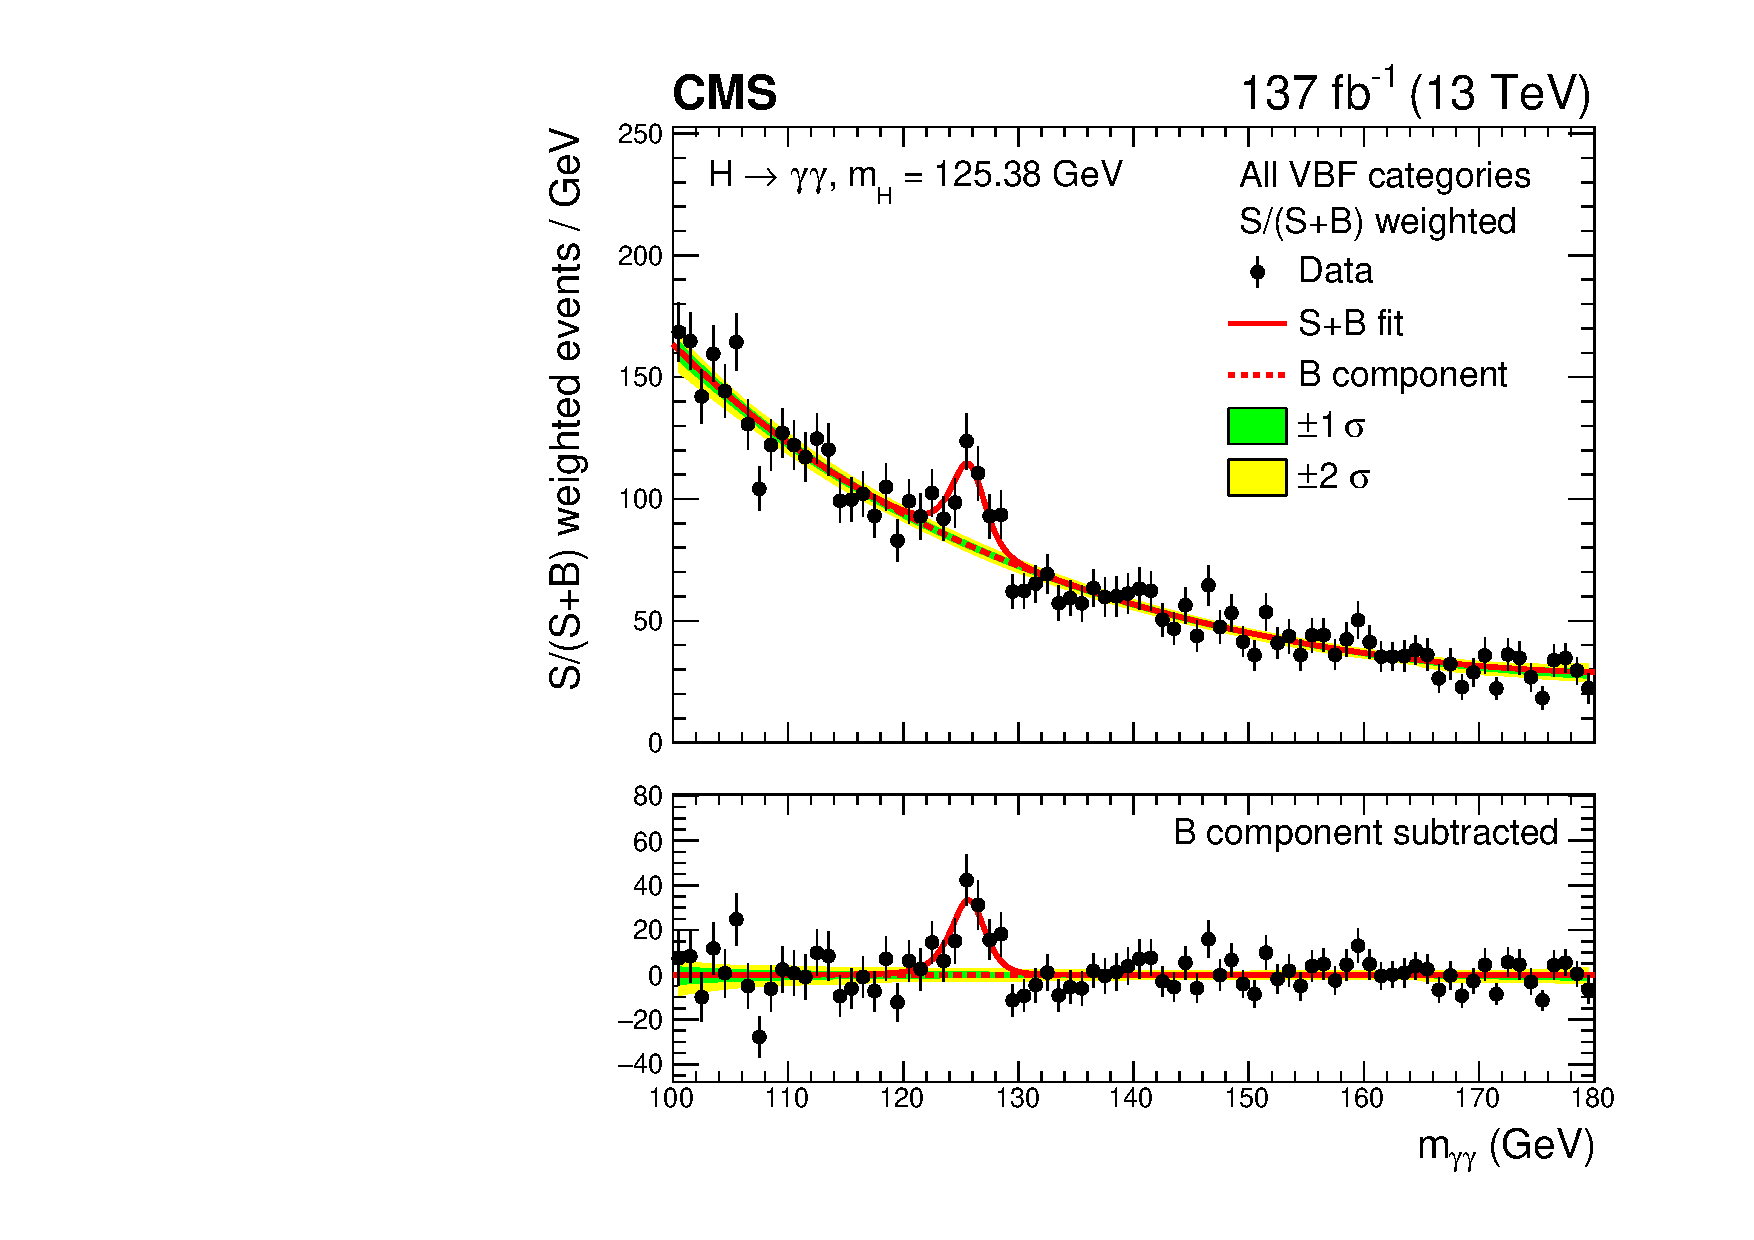
\includegraphics[width=.49\textwidth]{Figures/hgg_results/sPlusBweighted_VBF.pdf}
  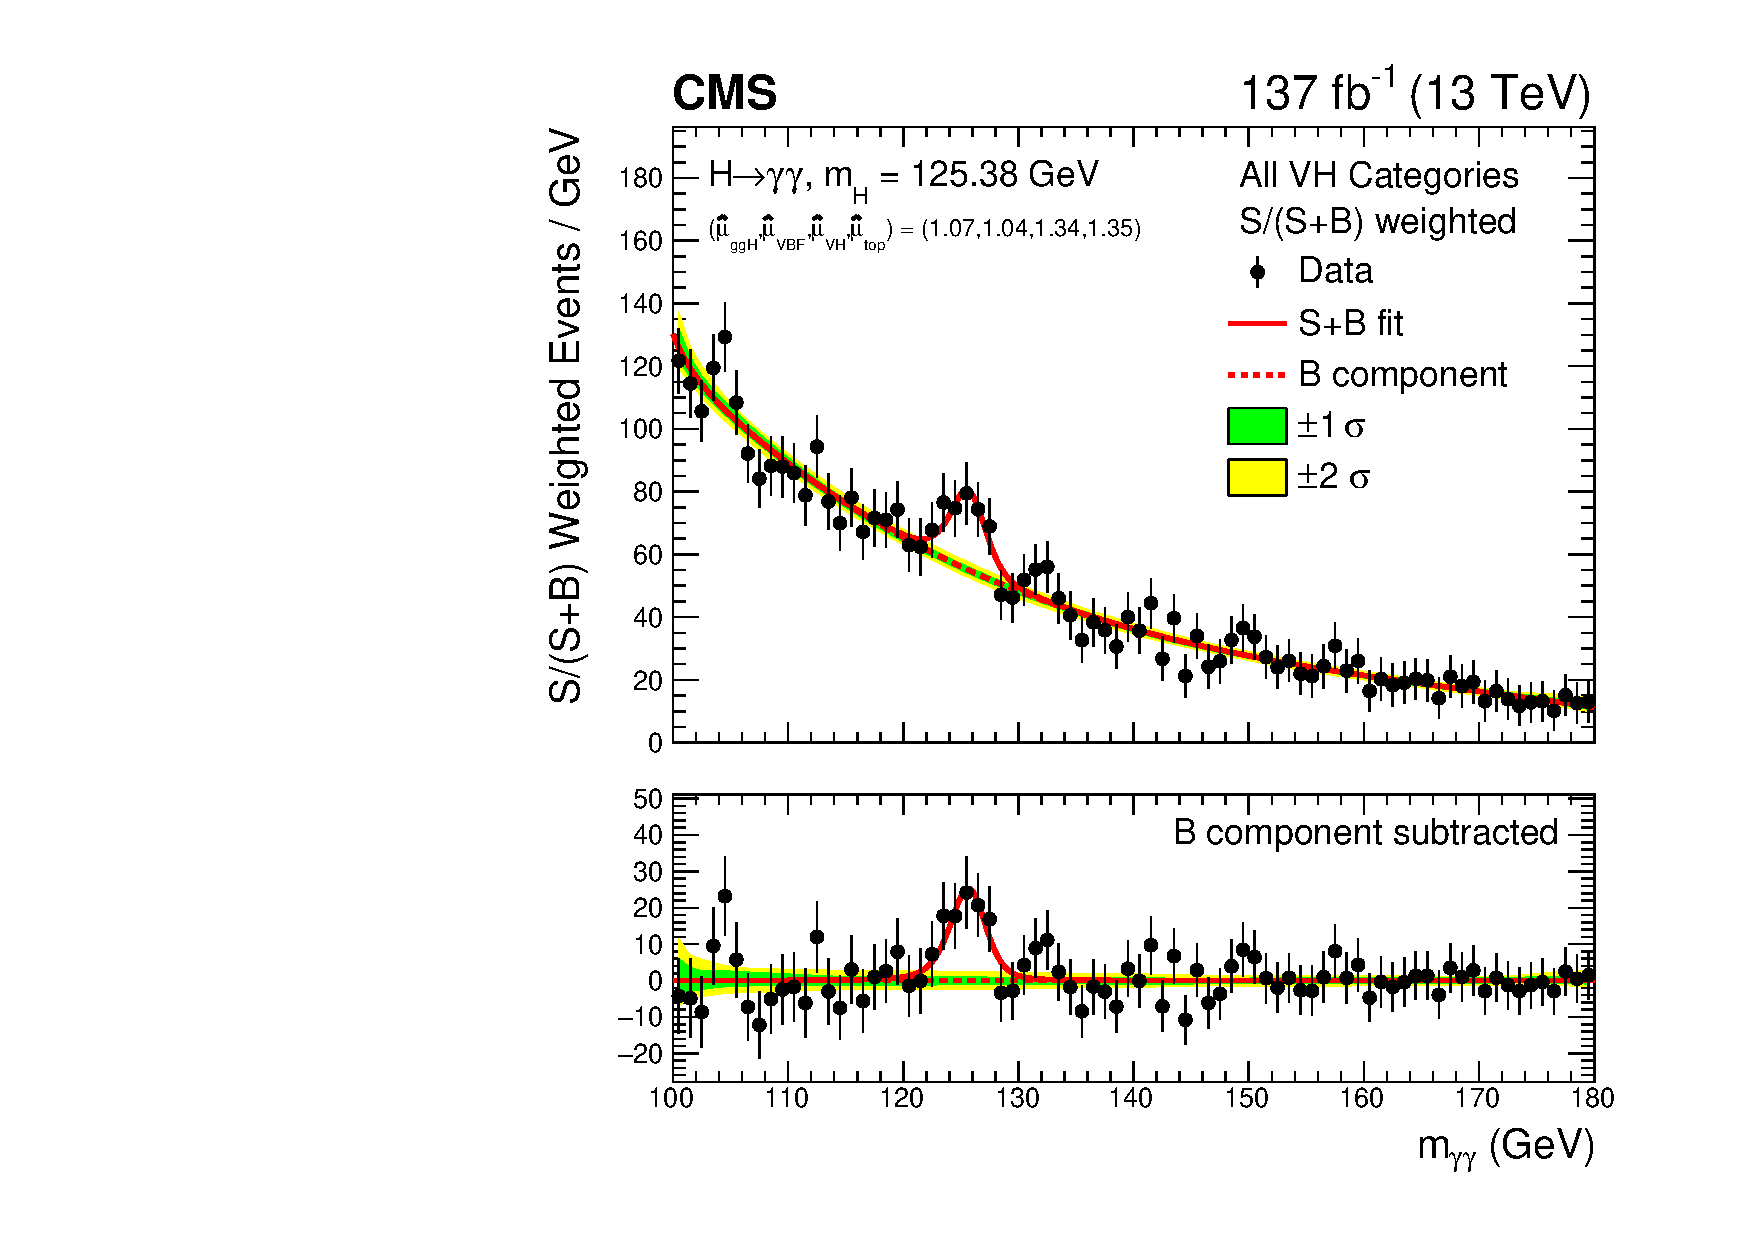
\includegraphics[width=.49\textwidth]{Figures/hgg_results/sPlusBweighted_VH.pdf}
  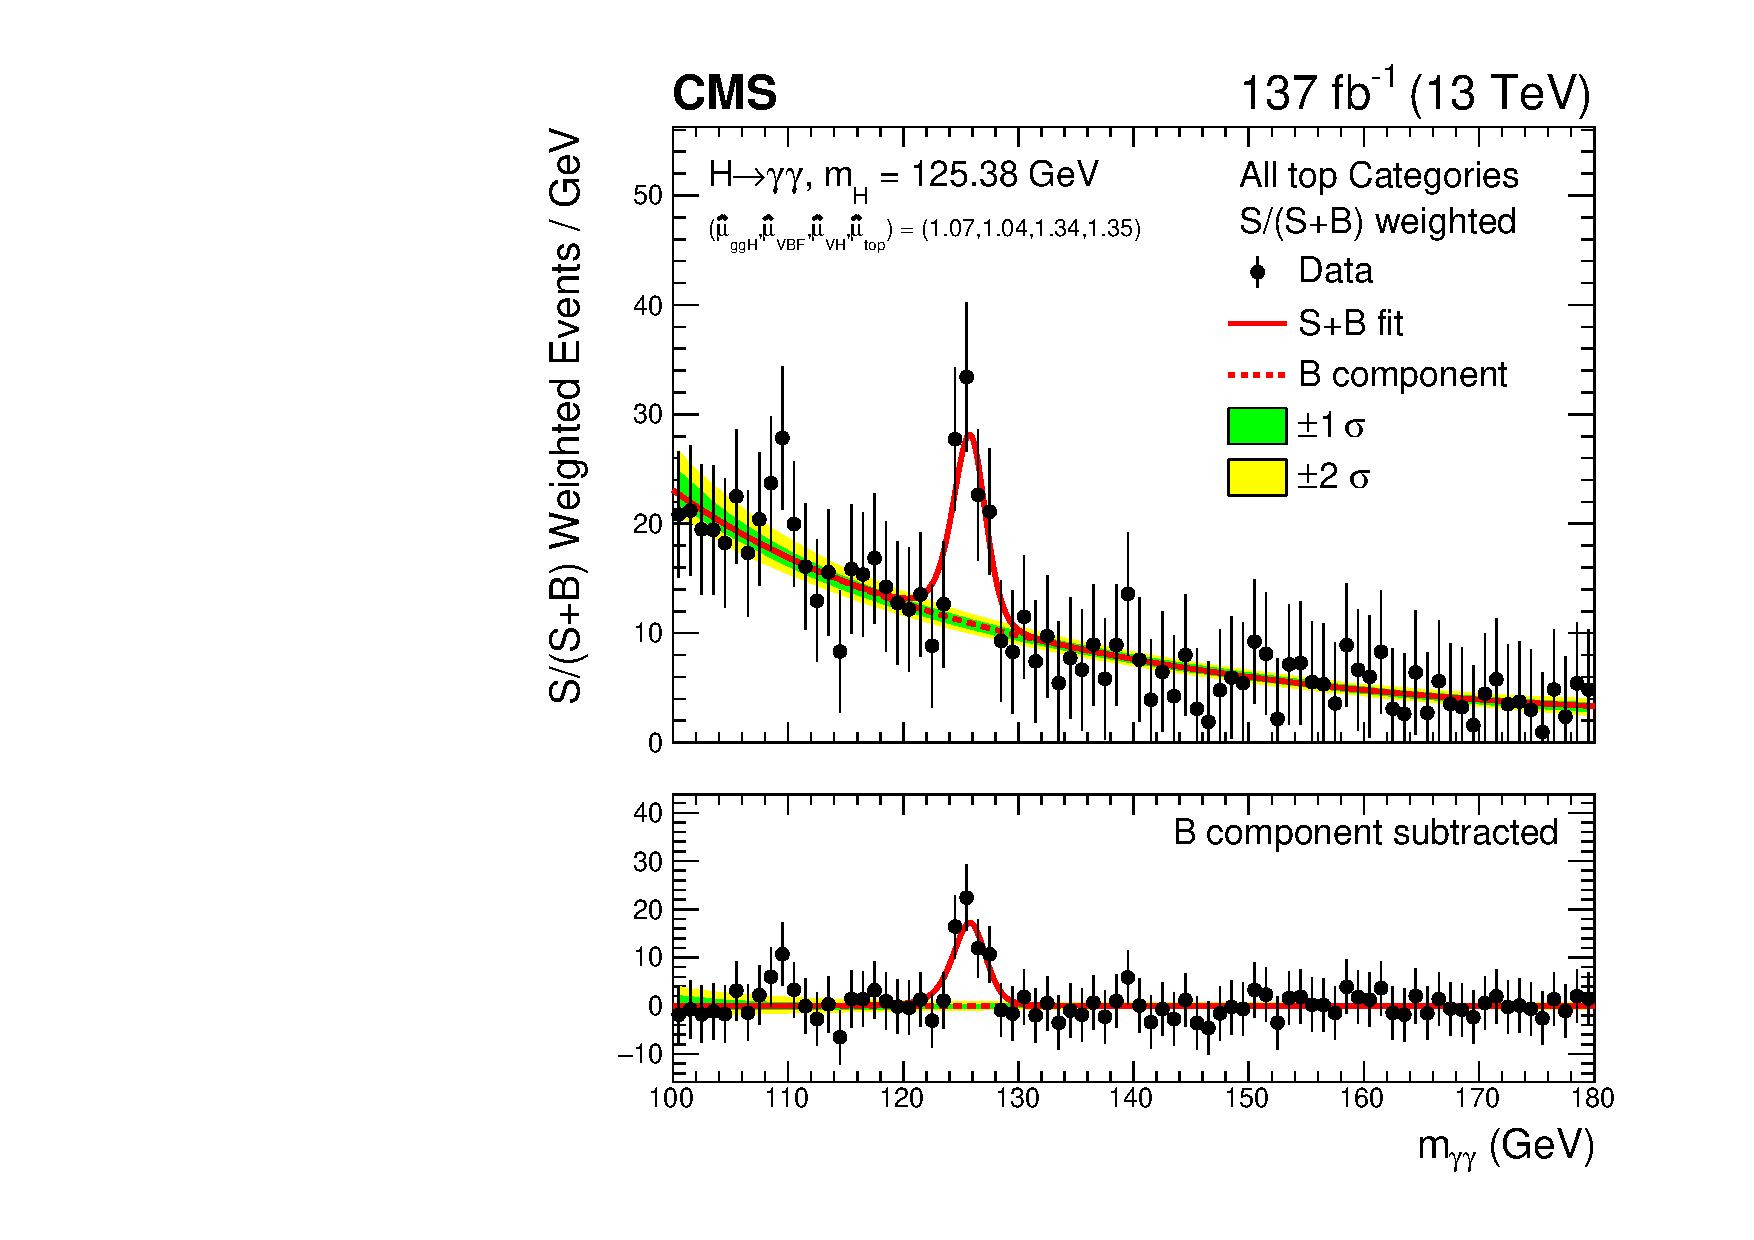
\includegraphics[width=.49\textwidth]{Figures/hgg_results/sPlusBweighted_top.pdf}
  \caption[Observed diphoton mass distribution for groups of categories targeting different Higgs boson production modes]
  {
    Data points (black) and the best-fit signal-plus-background model for groups of analysis categories targeting ggH (top-left), VBF (top-right), VH (bottom-left) and top-associated (bottom-right) production. The best-fit model corresponds to the per-production mode signal strength fit. In each category group, the events in each individual category are weighted according to $S_{68}/(S_{68}+B_{68})$, where $S_{68}$ and $B_{68}$ are the expected signal and background estimates, respectively, in a $\pm$1$\sigma_{\rm{eff}}$ window centred on $m_H$, such that the total signal yield in each category group remains constant. The solid red line shows the best-fit signal-plus-background model, whereas the dashed line shows the background component only. The one standard deviation (green) and two standard deviation (yellow) bands show the uncertainties in the background component of the fit. The bottom panels in each plot show the residuals after subtraction of this background component.
  }
  \label{fig:sb_mu}
\end{figure}

The best-fit values of the per-production mode signal strength modifiers and their respective uncertainties are summarised in Figure~\ref{fig:summary_mu}. Again, the uncertainties are decomposed into the theoretical systematic, experimental systematic, and statistical components. For $\mu_{\rm{ggH}}$, the systematic and statistical uncertainties are comparable, whereas for other parameters the dominant source of uncertainty is statistical in origin. All production modes are observed to have a signal strength larger than unity. Nevertheless, the results are compatible with the SM prediction, corresponding to a $p$-value of $p_{\rm{SM}}=50\%$.

\begin{figure}[htb!]
  \centering
  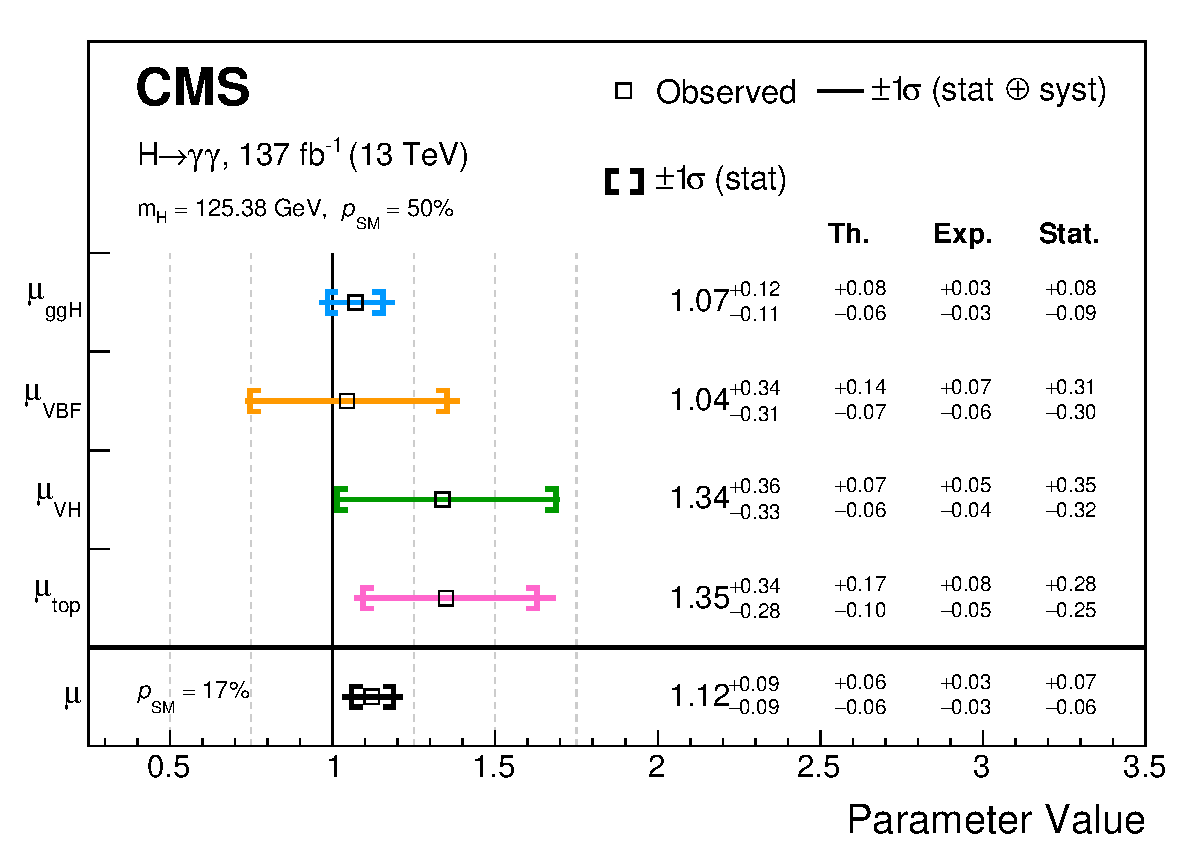
\includegraphics[width=1\textwidth]{Figures/hgg_results/mu_summary.pdf}
  \caption[Summary of the signal strength fit results]
  {
    Observed best-fit values and confidence intervals for the per-production mode signal strength parameters. The uncertainty bands are shown for including all systematic uncertainties, and the statistical uncertainty only. In addition, the results are tabulated, where the systematic uncertainty is further decomposed into the contributions from theoretical and experimental sources. Also shown in black is the result of the inclusive signal strength modifier fit.
  }
  \label{fig:summary_mu}
\end{figure}

The correlation coefficients between the fitted parameters are displayed in Figure \ref{fig:corr_mu}. The correlations are in general small, with the largest value of -0.20 occurring between the $\mu_{\rm{ggH}}$ and $\mu_{\rm{VBF}}$ parameters due to the contamination of VBF events in the analysis categories targeting ggH and vice versa. 

Finally, the main sources of systematic uncertainty affecting each production mode signal strength modifier are presented in Figure~\ref{fig:syst_mu}. The impact from each source, or group of sources, is derived using the procedure detailed in section \ref{sec:effect_of_nuisance}. The top half of the plot shows the experimental sources of uncertainty, whereas the bottom half shows the theoretical sources of uncertainty, including the impact of the $\vec{\theta}^{\,\rm{th}}_{s}$ nuisance parameters which are directly folded into the measurement in the signal strength parametrisation. The dominant contributions to the uncertainties in the measured parameters are theoretical in origin. For the $\mu_{\text{ggH}}$, $\mu_{\text{VH}}$ and $\mu_{\text{top}}$ parameters, the largest impact comes from the corresponding renormalisation and factorisation scale uncertainties. For $\mu_{\text{VBF}}$, the dominant source of uncertainty is in the modelling of the underlying event and parton shower. These are particularly important for VBF production due to the presence of additional jets in the events. The largest experimental uncertainties originate from the integrated luminosity, the photon identification, and the photon energy measurement for the $\mu_{\text{ggH}}$ and $\mu_{\text{VH}}$ parameters. The uncertainties in the jet energy scale and resolution have a larger impact on $\mu_{\text{VBF}}$ and $\mu_{\text{top}}$, where $\mu_{\text{top}}$ has an additional large contribution from the uncertainty in the b tagging.

\begin{figure}[htb!]
  \centering
  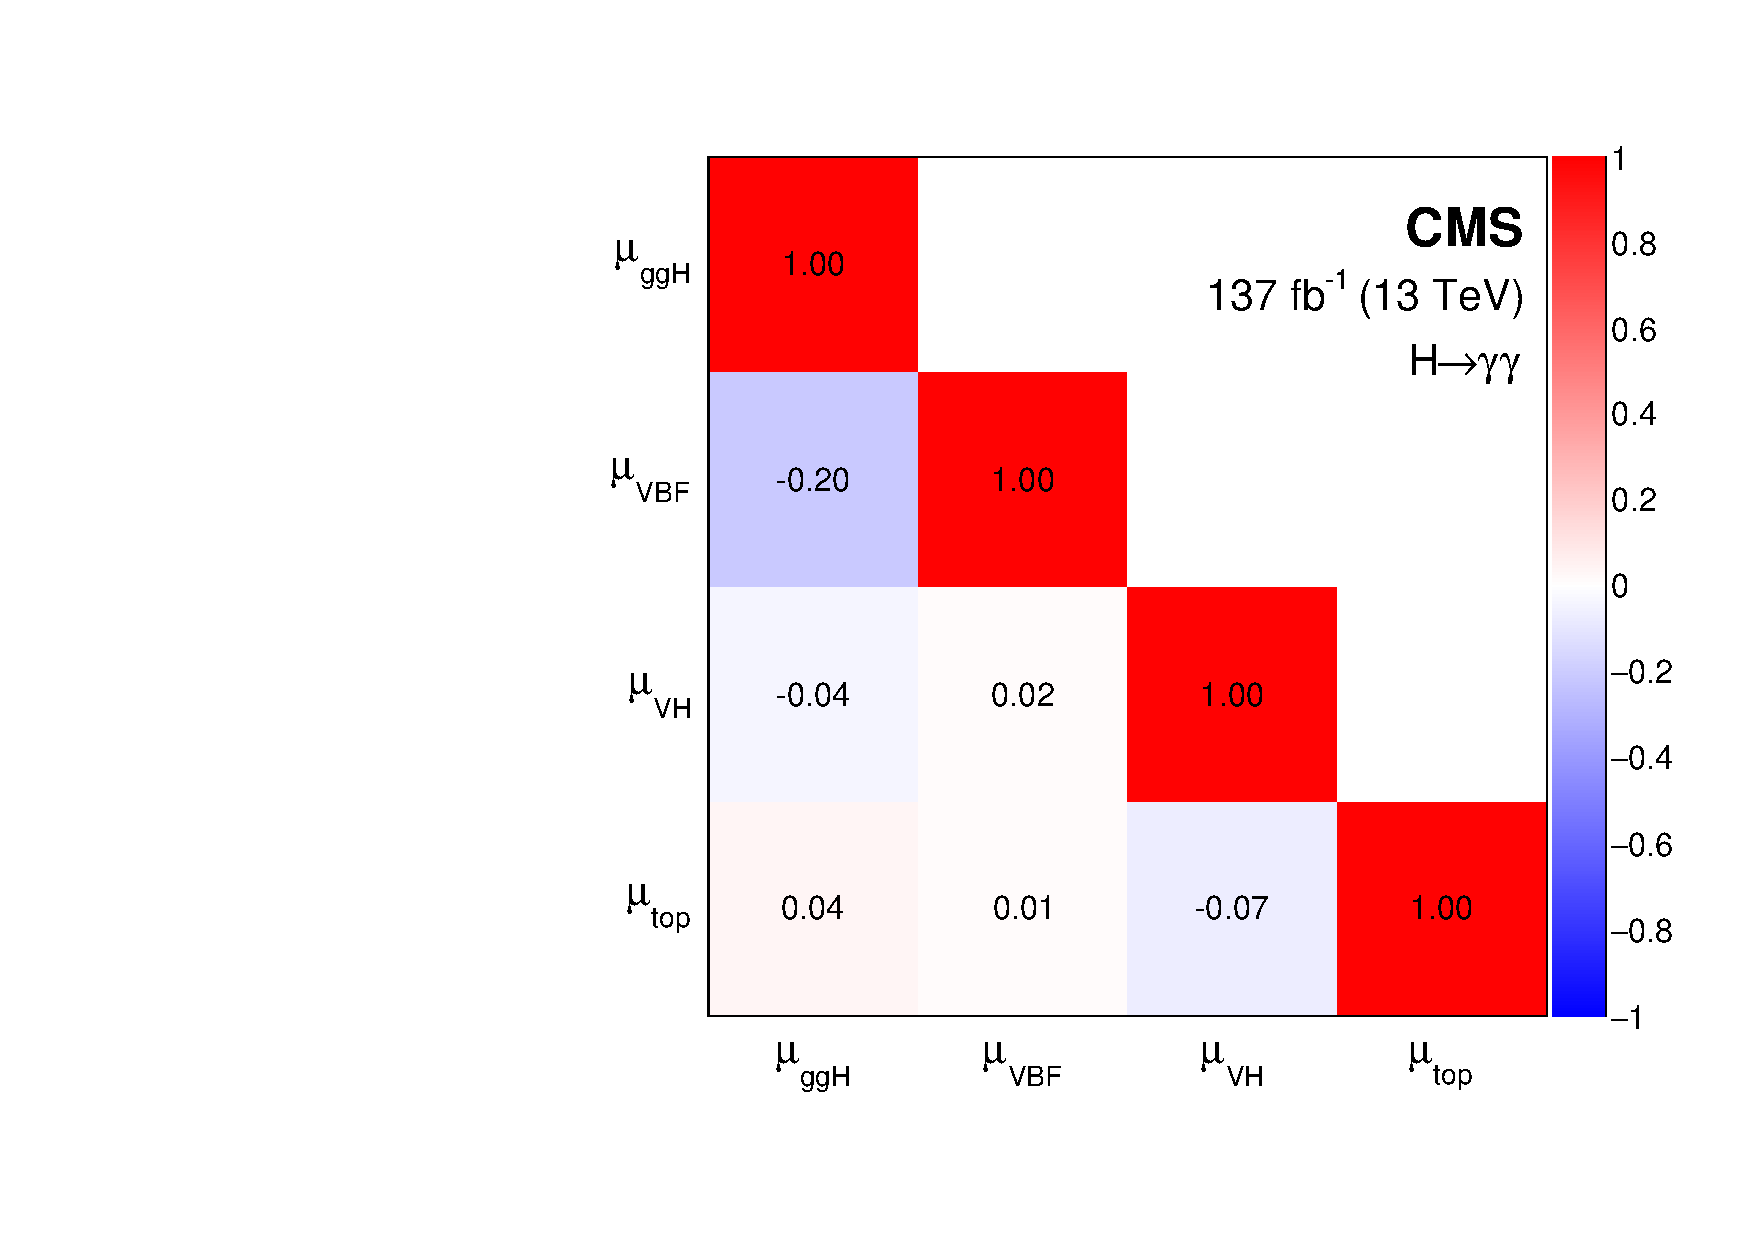
\includegraphics[width=.7\textwidth]{Figures/hgg_results/mu_correlations.pdf}
  \caption[Correlations between per-production mode signal strengths]
  {
    Observed correlations between the parameters in the per-production mode signal strength fit. The size of the correlations is indicated by the colour scale.
  }
  \label{fig:corr_mu}
\end{figure}

\begin{figure}[htb!]
  \centering
  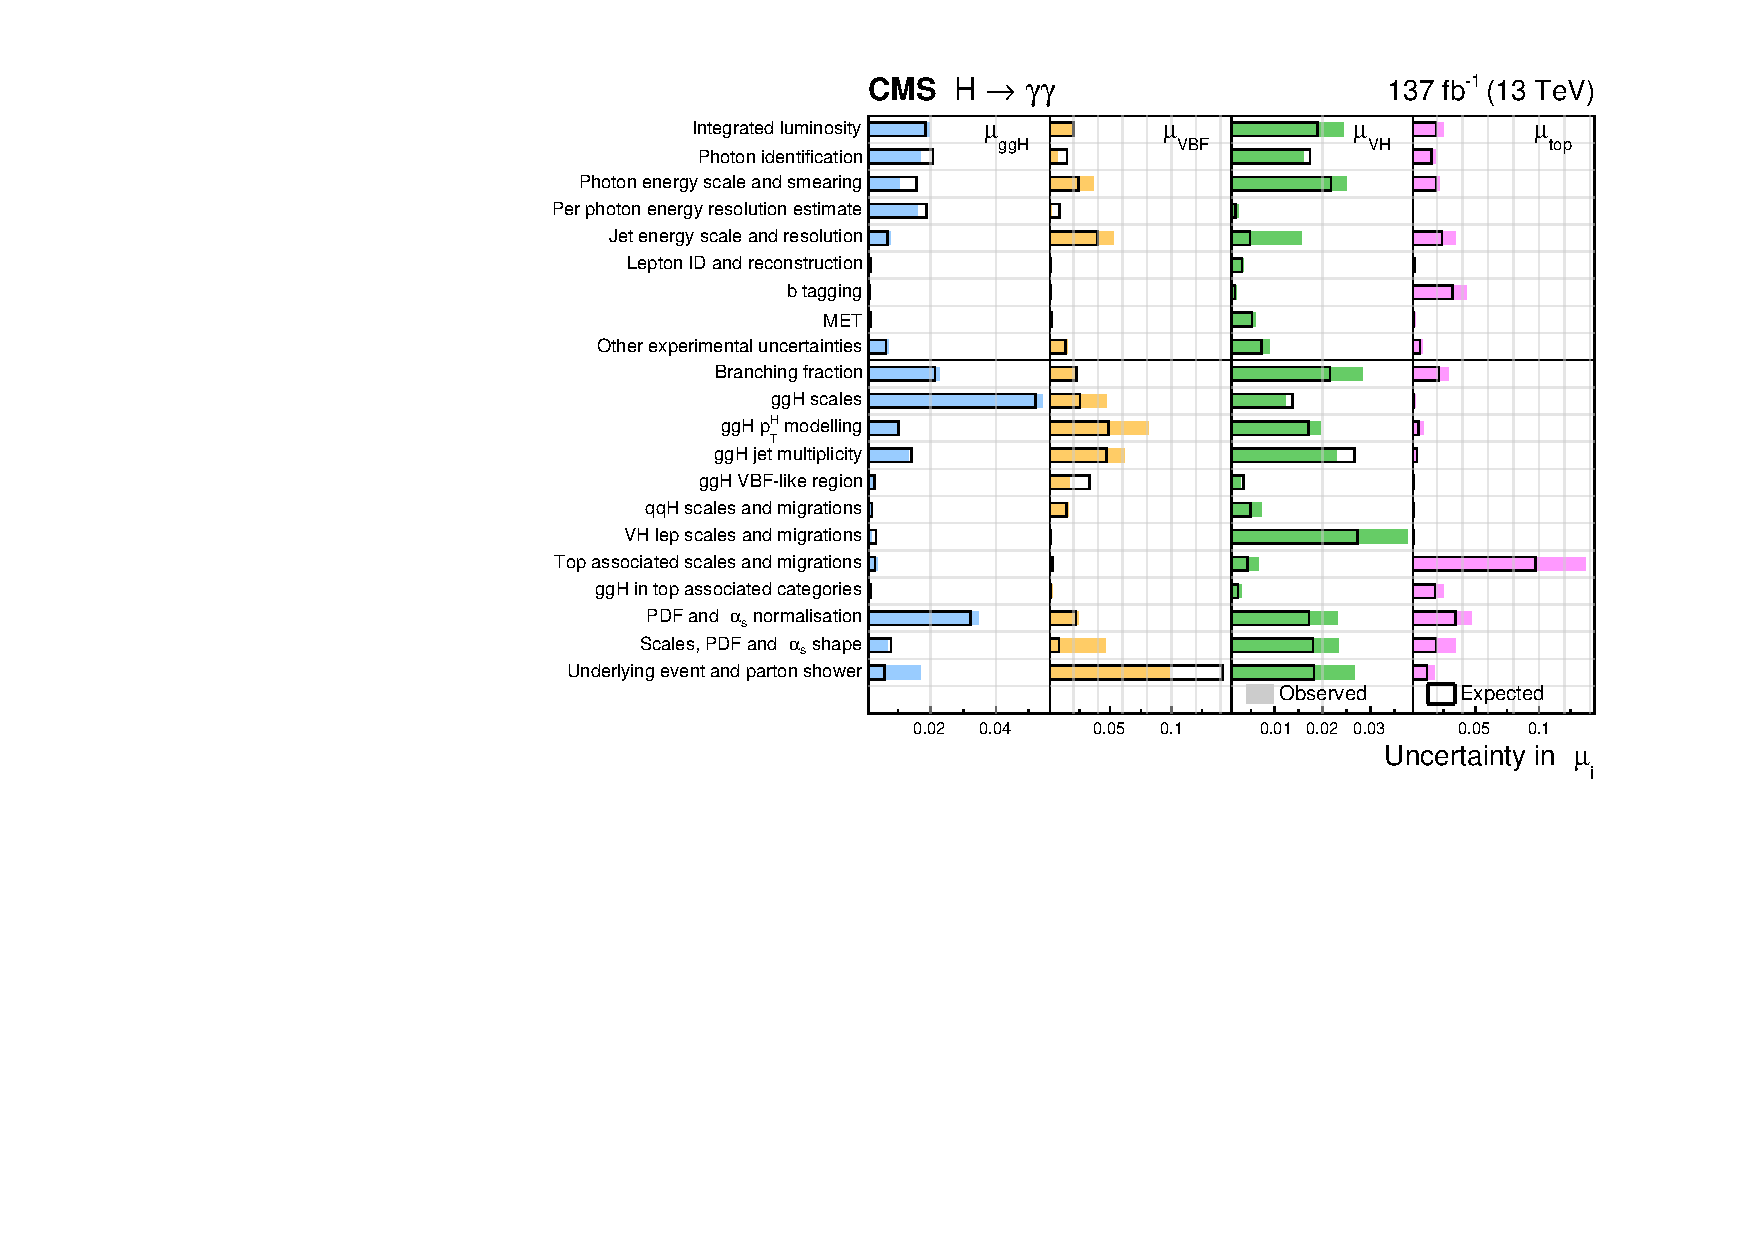
\includegraphics[width=1\textwidth]{Figures/hgg_results/mu_systematics.pdf}
  \caption[Impact of systematic uncertainty sources on the per-production mode signal strengths]
  {
    A summary of the absolute impact of the main sources of systematic uncertainty in the four parameters: $\mu_{\rm{ggH}}$, $\mu_{\rm{VBF}}$, $\mu_{\rm{VH}}$, $\mu_{\rm{top}}$. The uncertainties are split into experimental (top half) and theoretical (bottom half) sources. The obseved (expected) impacts are shown by the solid (empty) bars.
  }
  \label{fig:syst_mu}
\end{figure}

\FloatBarrier
% \newpage
\section{STXS measurements}\label{sec:results_STXS}
This section describes the extraction of cross sections in the STXS framework and their respective 68\% confidence intervals and correlation coefficients. The event categorisation, described in section \ref{sec:event_categorisation}, is optimised to measure as many STXS stage 1.2 bins as possible. Nevertheless, given the current available statistics, it is not possible to accurately measure all bins simultaneously using the \Hgg decay channel alone. Three STXS bin merging schemes are defined with varying levels of granularity to ensure reasonable sensitivity to the measured parameters, and avoid very high correlations between them. In the construction of the schemes there is a trade-off between model-dependence and the size of uncertainties. Merging fewer bins keeps the model-dependence as low as possible, as no additional assumptions are made about the relative contributions of different STXS bins. However, this reduced model-dependence comes at the cost of larger uncertainties in the measured cross section parameters.

In contrast to the signal strength fits, the VH hadronic processes are grouped with VBF production to define the qqH parameters (see section \ref{sec:theory_stxs}), and bbH and ggZH production in which the Z boson decays hadronically are grouped with ggH. Furthermore, the theory uncertainty treatment is different to the signal strength and coupling modifier fits. This difference reflects the distinction between cross section \textit{measurements} and \textit{interpretations}. Nuisance parameters that directly affect the SM predictions of the cross sections and branching fraction cancel in equation \ref{eq:signal_yield}, and therefore are not included in the measurements. That said, when merging STXS bins and thus re-defining the signal processes, it is necessary to introduce the relevant $\theta^{\,\rm{th}}_{s}$ nuisance parameter that accounts for the migration of events across the merged boundary. 

In each fit the cross section parameters are limited to the positive domain: $\sigma_{\rm{obs}}\geq0$~fb. This eliminates the possibility of the signal-plus-background model going below zero in some bins of the \mgg distributions, which subsequently causes the minimisation procedure to fail.

\subsection{STXS stage 0}
A fully-merged fit is performed, corresponding to the STXS stage 0 bin definitions~\cite{deFlorian:2016spz}. The parameters of interest roughly correspond to the different Higgs boson production modes, such that all kinematic boundaries for a given production mode are merged. This scheme defines six parameters in total: ggH, qqH, WH lep, ZH lep, ttH, and tH, where tH includes the contributions from both tHq and tHW production. The best-fit values of the cross sections times branching fraction, \xsbr, and their respective 68\% confidence levels are shown in Figure \ref{fig:stage0_results}. In the plot, the colour scheme has been chosen to match the STXS bin schematic in Figure \ref{fig:stxs_schematic}. The systematic components of the measured uncertainties are shown by the coloured boxes, highlighting that for all parameters except ggH, the statistical uncertainty dominates. The 68\% uncertainties in the SM predicted values are shown by the hatched grey boxes, where the size of the uncertainty is computed by adding the effect of the $\vec{\theta}^{\,\rm{th}}_{s}$ nuisance parameters which do not enter the measurement in quadrature.

All measurements are consistent with the SM predicted values within one standard deviation, barring the tH parameter which is measured to have an excess of around six times the SM prediction. Despite this, the low expected tH event yield results in a large statistical uncertainty, meaning the excess corresponds to a less than 2$\sigma$ deviation from the SM. The overall compatibility with the SM is measured to be $p_{\rm{SM}}=35\%$. The correlation coefficients between parameters are displayed in Figure \ref{fig:stage0_correlations}. The largest (anti-)correlation exists between the ttH and tH parameters, due to the significant contamination of ttH in the tHq leptonic analysis category.

Importantly, this is the first dedicated measurement of single-top associated production in the \Hgg channel at CMS. The observed (expected) limit on tH production at 95\% $\rm{CL}$, using the $\rm{CL}_s$ procedure detailed in Ref.~\cite{CMS-NOTE-2011-005}, is 14 (8) times the SM expectation. This represents one of the most stringent constraints on tH production to-date.

\begin{figure}[htb!]
  \centering
  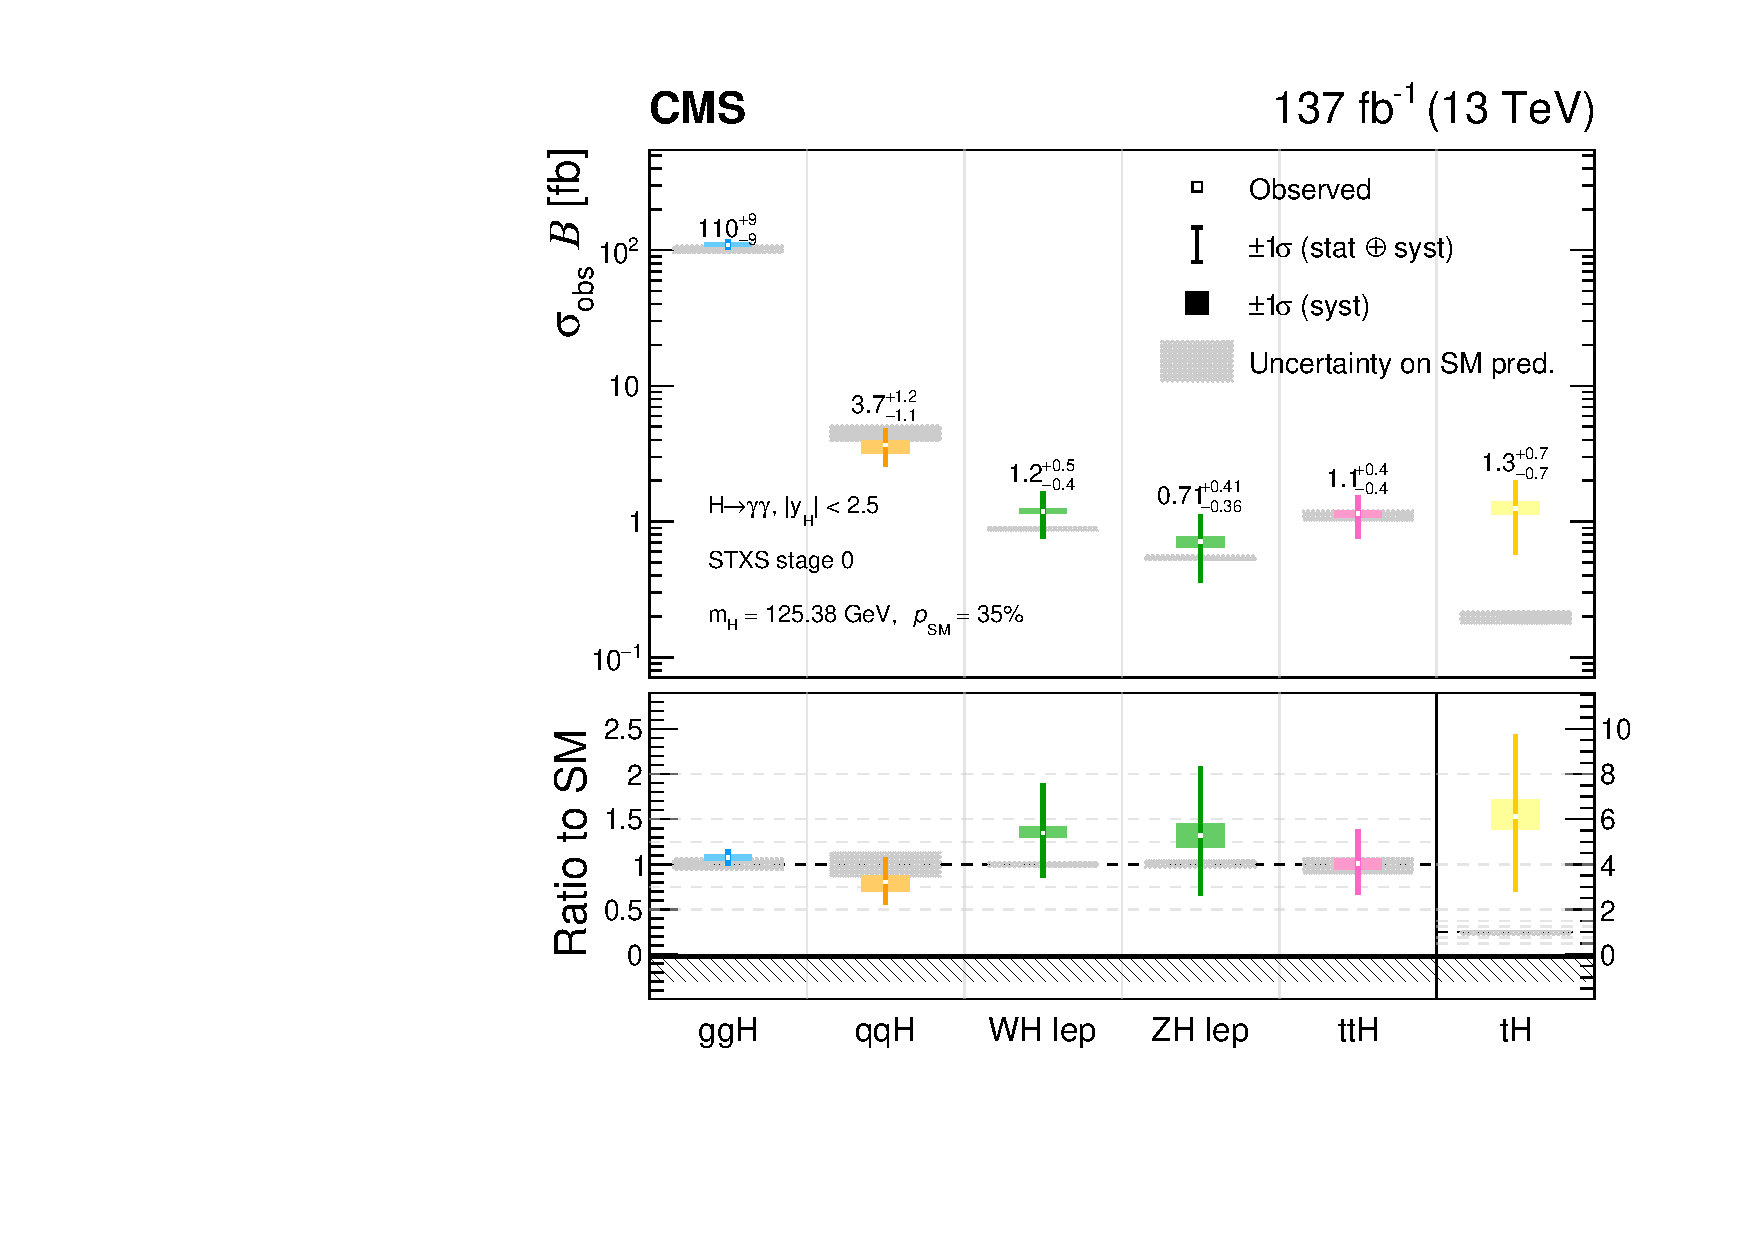
\includegraphics[width=.6\textwidth]{Figures/hgg_results/stage0_summary.pdf}
  \caption[Results of the STXS stage 0 fit]
  {
    Observed results of the STXS stage 0 fit. The best fit cross sections times branching fraction are plotted along with the respective 68\% confidence intervals. The systematic components of the uncertainty in each parameter are shown by the coloured boxes. The hatched grey boxes represent the theoretical uncertainty in the SM predictions. The bottom panel shows the ratio of the fitted values to the SM predictions. The compatibility of this fit with the SM prediction is approximately $p_{\rm{SM}}=35\%$. 
  }
  \label{fig:stage0_results}
\end{figure}

\begin{figure}[htb!]
  \centering
  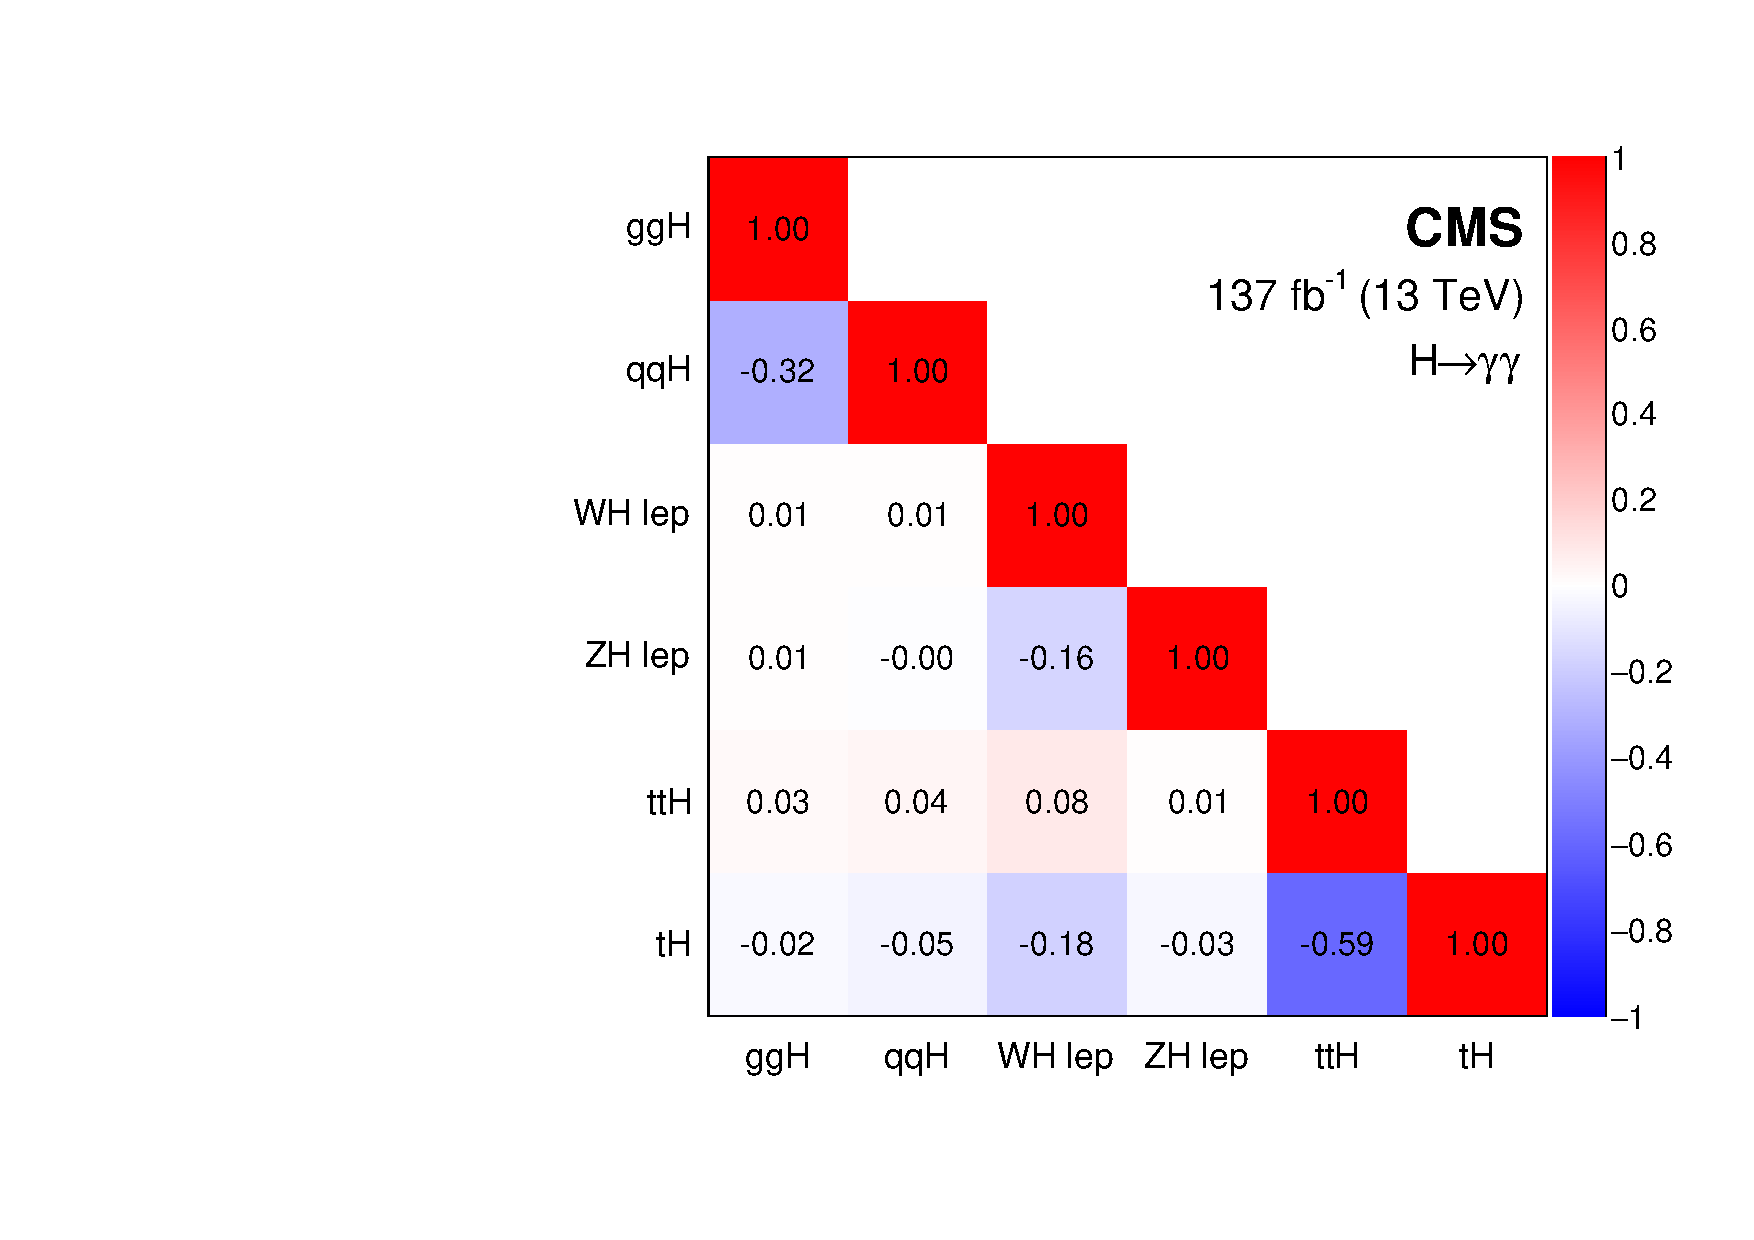
\includegraphics[width=.55\textwidth]{Figures/hgg_results/stage0_correlations.pdf}
  \caption[Correlations in the STXS stage 0 parameters]
  {
    Observed correlations between the six parameters in the STXS stage 0 fit. The size of the correlations is indicated by the colour scale.
  }
  \label{fig:stage0_correlations}
\end{figure}

\FloatBarrier
\subsection{Maximal merging scheme}
\begin{figure}[htb!]
  \centering
  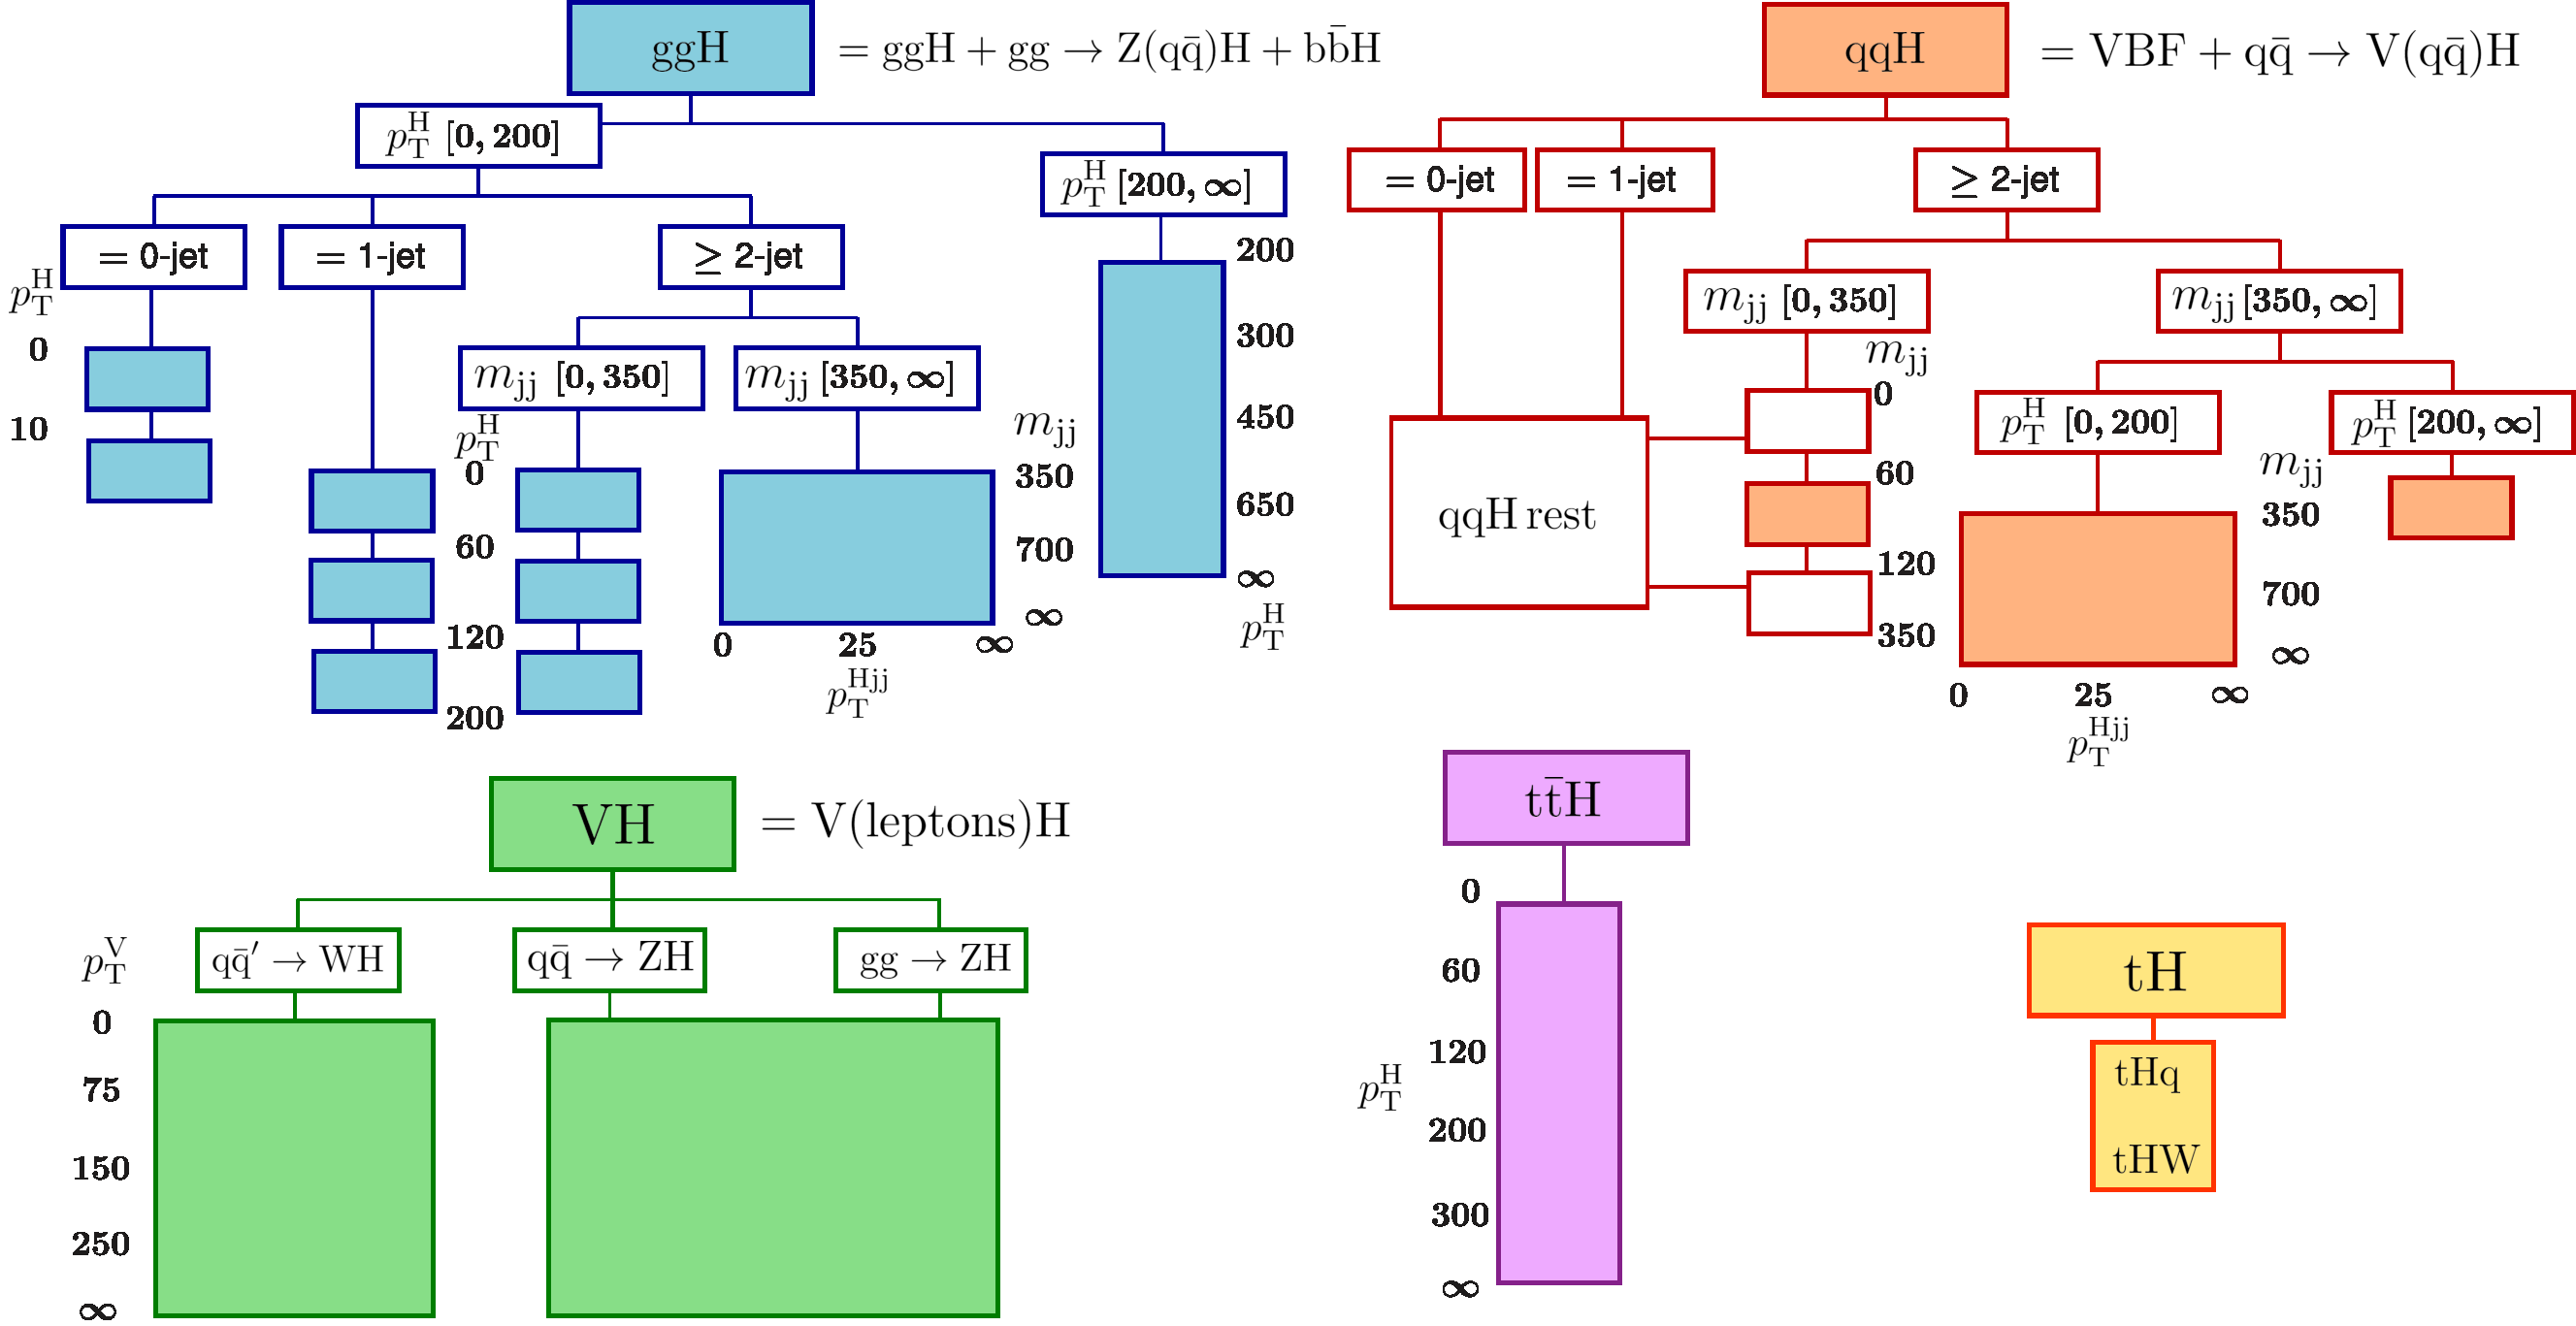
\includegraphics[width=1\linewidth]{Figures/app_merging_schemes/allSTXSbins_maximal.pdf}
  \caption[Schematic of the maximal merging scheme]
  {
    Schematic to show the maximal merging scheme which defines 17 parameters of interest. Each parameter of interest is shown as a single coloured box.
  }
  \label{fig:maximal_scheme}
\end{figure}

Increasing in granularity, the \textit{maximal merging scheme} defines 17 parameters of interest which begin to target a number of the STXS kinematic splittings. In the scheme, bins are merged until their expected uncertainty is less than 150\% of the SM prediction. This is true for all parameters except tH, which is again measured separately. The VBF-like regions ($\geq$2J, $\mgg>350$~GeV) in the ggH and qqH schemes are merged to define the ggH VBF-like and qqH VBF-like parameters, respectively. The four bins with $\ptH>200$~GeV in the ggH scheme are merged into a single bin, labelled as ggH BSM. Additionally, the WH leptonic, ZH leptonic, and ttH bins are fully merged into single parameters. The ZH leptonic parameter groups both (qq-initiated) ZH lep and ggZH lep production. Due to a lack of constraining power, in this fit the 0J, 1J, $\mjj<60$ and $120<\mjj<350$ bins in the qqH binning scheme are constrained to their SM prediction within theory uncertainties. A schematic representation of the merging scheme is presented in Figure~\ref{fig:maximal_scheme}, whilst Appendix~\ref{app:merging_table} tabulates the STXS bins which contribute to each parameter.


\begin{figure}[htb!]
  \centering
  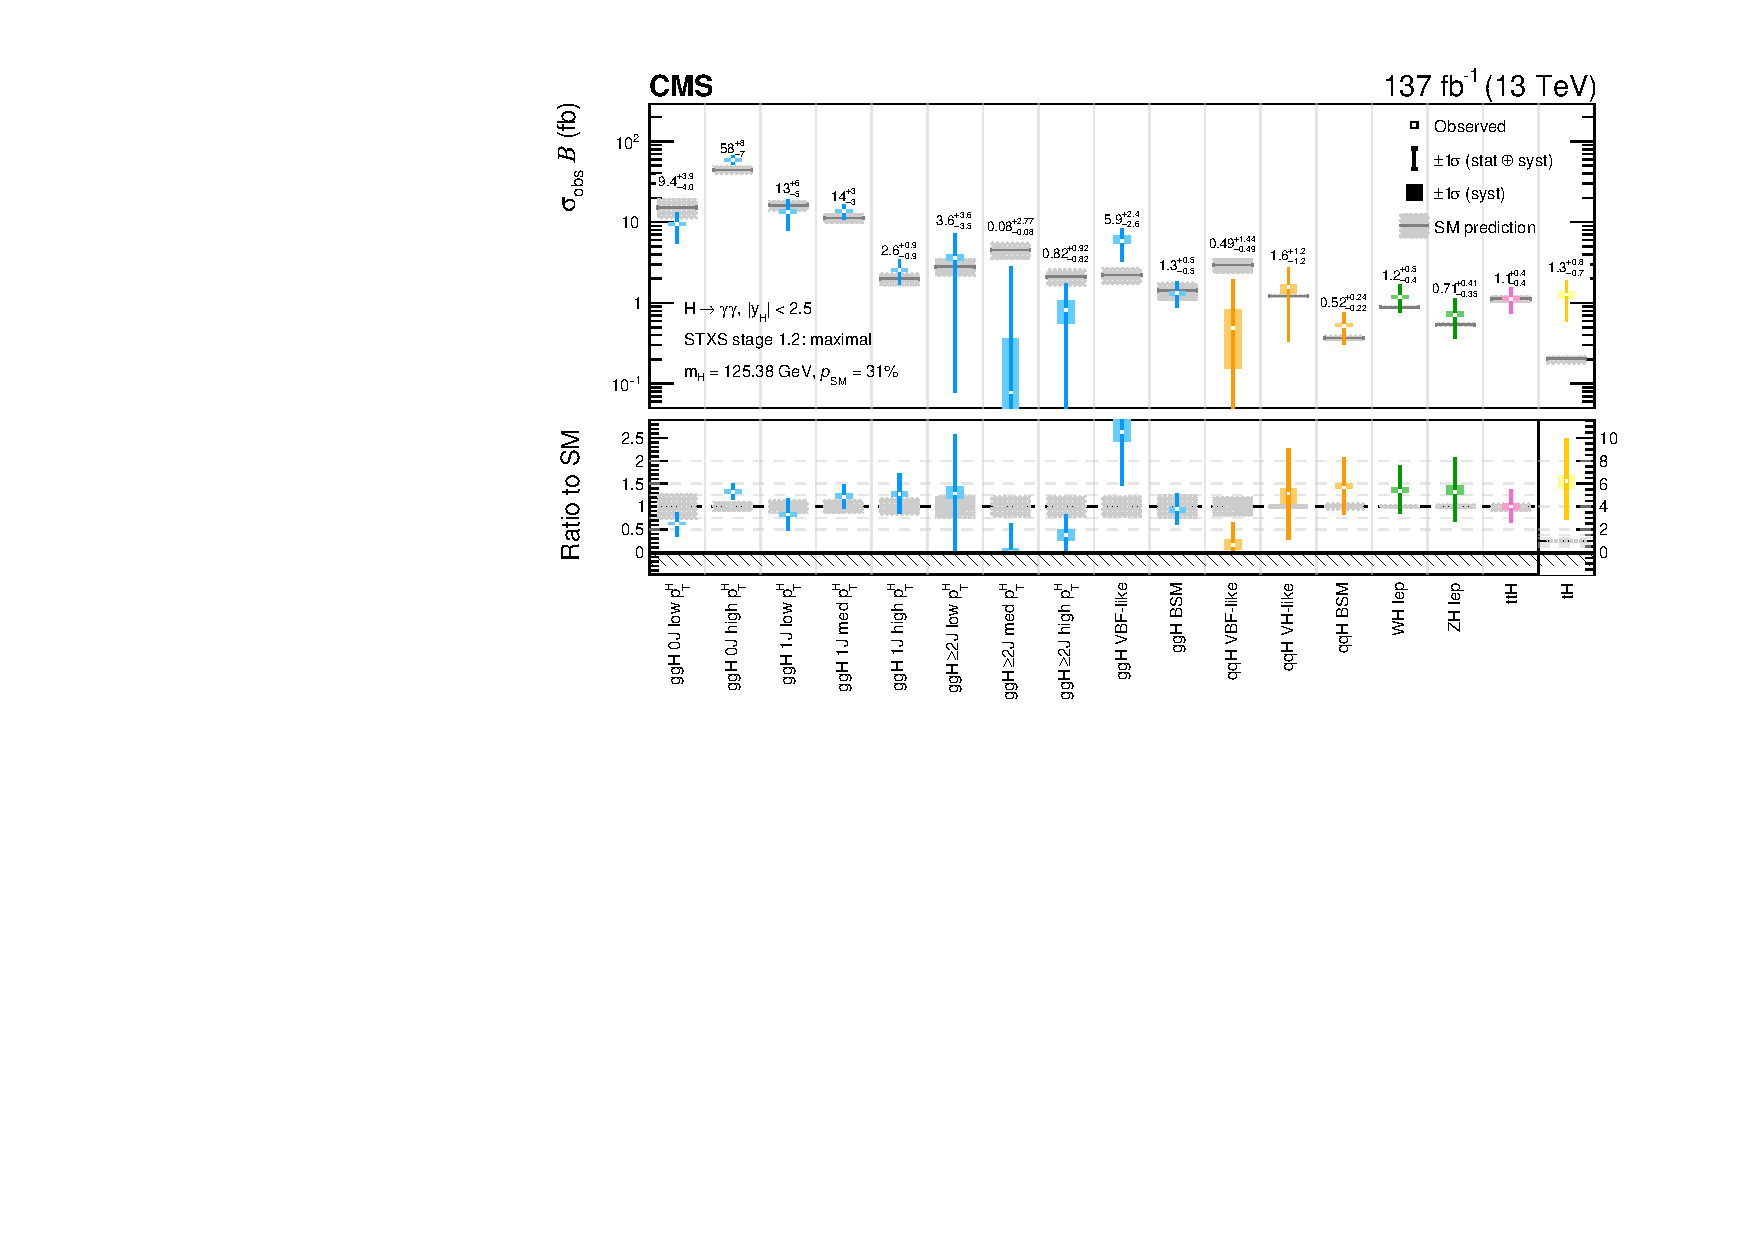
\includegraphics[width=1\textwidth]{Figures/hgg_results/stage1p2_maximal_summary.pdf}
  \caption[Results of the STXS stage 1.2 maximal merging fit]
  {
    Observed results of the STXS stage 1.2 maximal merging fit. The best fit cross sections times branching fraction are plotted along with the respective 68\% confidence intervals. The systematic components of the uncertainty in each parameter are shown by the coloured boxes. The hatched grey boxes represent the theoretical uncertainty in the SM predictions. The bottom panel shows the ratio of the fitted values to the SM predictions. The compatibility of this fit with the SM prediction is approximately $p_{\rm{SM}}=31\%$. 
  }
  \label{fig:stage1p2_maximal_results}
\end{figure}

Figure \ref{fig:stage1p2_maximal_results} shows the \xsbr best-fit values and 68\% confidence intervals in the maximal merging scheme, plotted in the same style as the STXS stage 0 results. With this level of kinematic splitting, the statistical component of the uncertainty dominates for all parameters. This motivates the need to increase the size of the dataset, which will in turn provide substantial improvements in the precision of the measured quantities. Moreover, for a number of parameters, the uncertainty in the measurement is becoming comparable to the uncertainty in the SM prediction, meaning the possibility of constraining Higgs boson theory using experimental measurements is approaching. This is especially interesting for the ggH BSM parameter, which is particularly sensitive to new physics in the ggH loop. That said, the measured value of the ggH BSM \xsbr is in excellent agreement with the SM, with a measured value of $0.9^{+0.4}_{-0.3}$, relative to the SM prediction. The overall compatibility with the SM is $p_{\rm{SM}}=31\%$. Table \ref{tab:stage1p2_maximal_results} summarises these results, providing in addition the expected uncertainties in the parameters, derived using the Asimov data set. 
%\textbf{Add impacts to main body/appendix.}

The correlation coefficients between the maximal merging parameters are shown in Figure \ref{fig:stage1p2_maximal_correlations}. For the ggH parameters, the correlations are as expected: small correlations for parameters representing adjacent \ptH bins but larger correlations for parameters representing adjacent $N_{\rm{jet}}$ bins. This stems from the fact that \ptgg is a well-measured quantity, whereas reconstructing the number of jets in an event is a more difficult problem. Nevertheless, the application of the ggH BDT in the event categorisation helps to reduce these correlations. The largest correlations exist between the qqH VBF-like and ggH VBF-like parameters (-0.76), and the tH and ttH parameters (-0.59). This results from the difficulty in distinguishing qqH from ggH production in the VBF-like phase space, and in distinguishing tH from ttH, attempted by the Dijet BDT and top DNN respectively. Two dimensional likelihood scans are performed for each pair of highly-correlated parameters to gain a better understanding of the impact of their correlations on the total $q(\vec{\alpha})$ surface. The 68\% and 95\% confidence regions are plotted for ggH VBF-like vs qqH VBF-like (left) and tH vs ttH (right) in Figure \ref{fig:2d_maximal}. In the scans, all other maximal merging parameters are profiled. Both scans show compatibility with the SM within the 95\% confidence contour.

\begin{figure}[htb!]
  \centering
  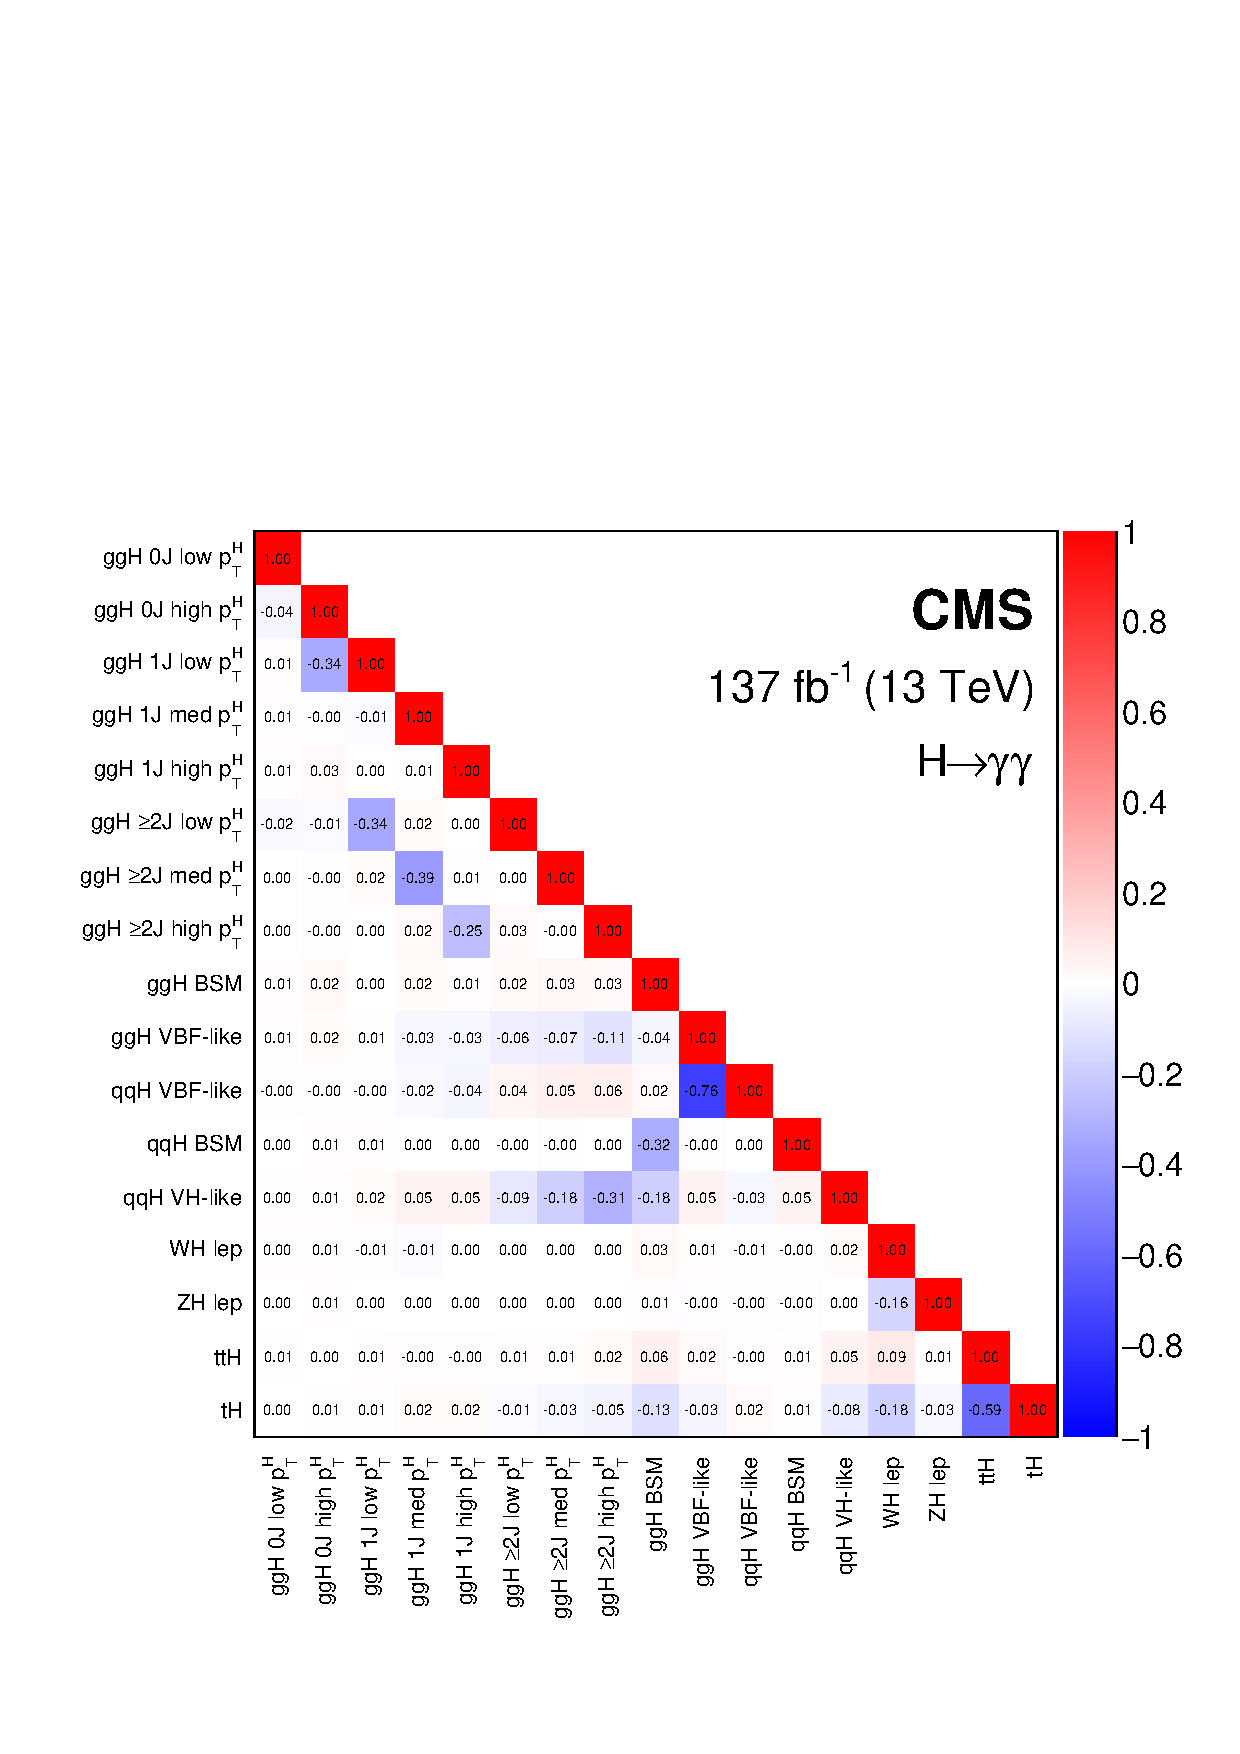
\includegraphics[width=.75\textwidth]{Figures/hgg_results/stage1p2_maximal_correlations.pdf}
  \vspace{-.5cm}
  \caption[Correlations in the STXS stage 1.2 maximal merging parameters]
  {
    Observed correlations between the 17 parameters in the STXS stage 1.2 maximal merging fit. The size of the correlations is indicated by the colour scale.
  }
  \label{fig:stage1p2_maximal_correlations}
\end{figure}

\begin{figure}[htb!]
  \centering
  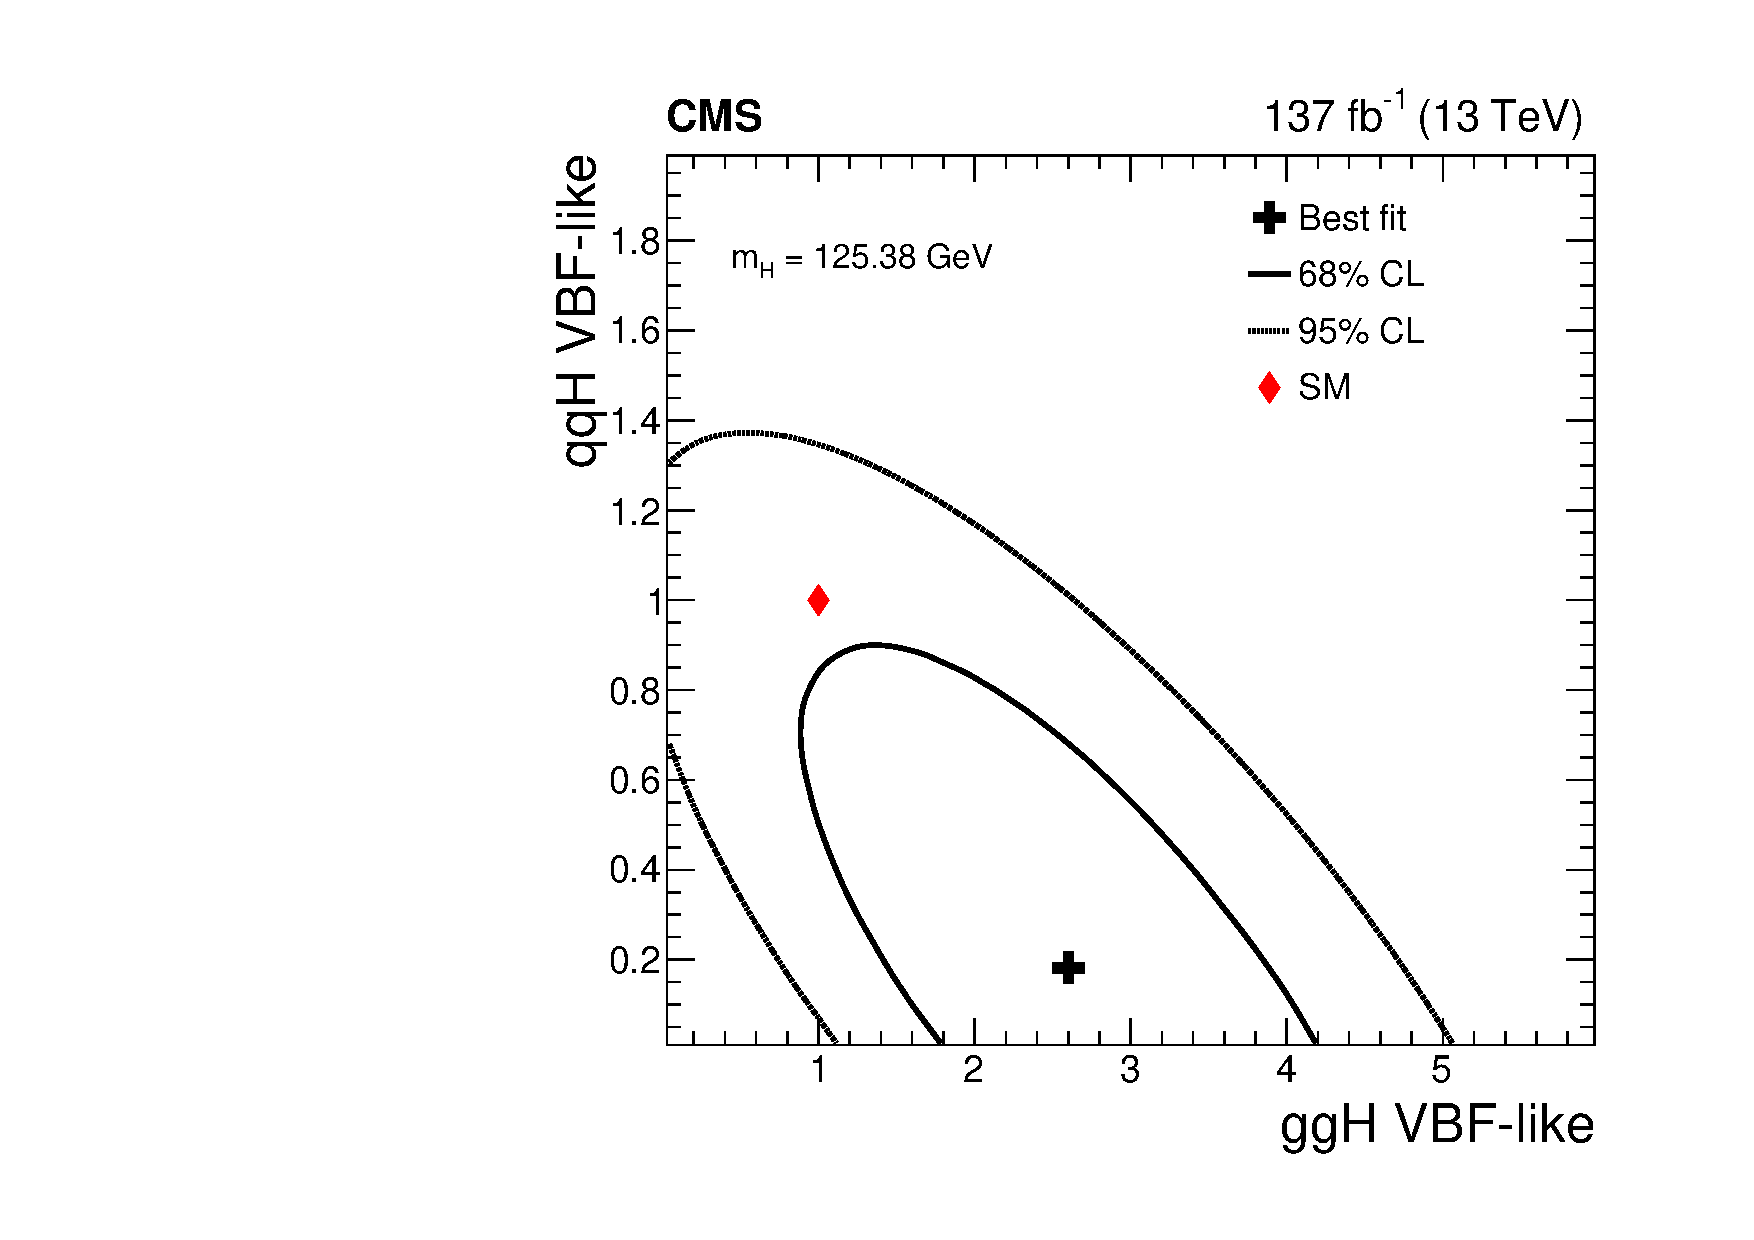
\includegraphics[width=.4\textwidth]{Figures/hgg_results/scan2D_r_ggH_VBFlike_vs_r_qqH_VBFlike_obs.pdf}
  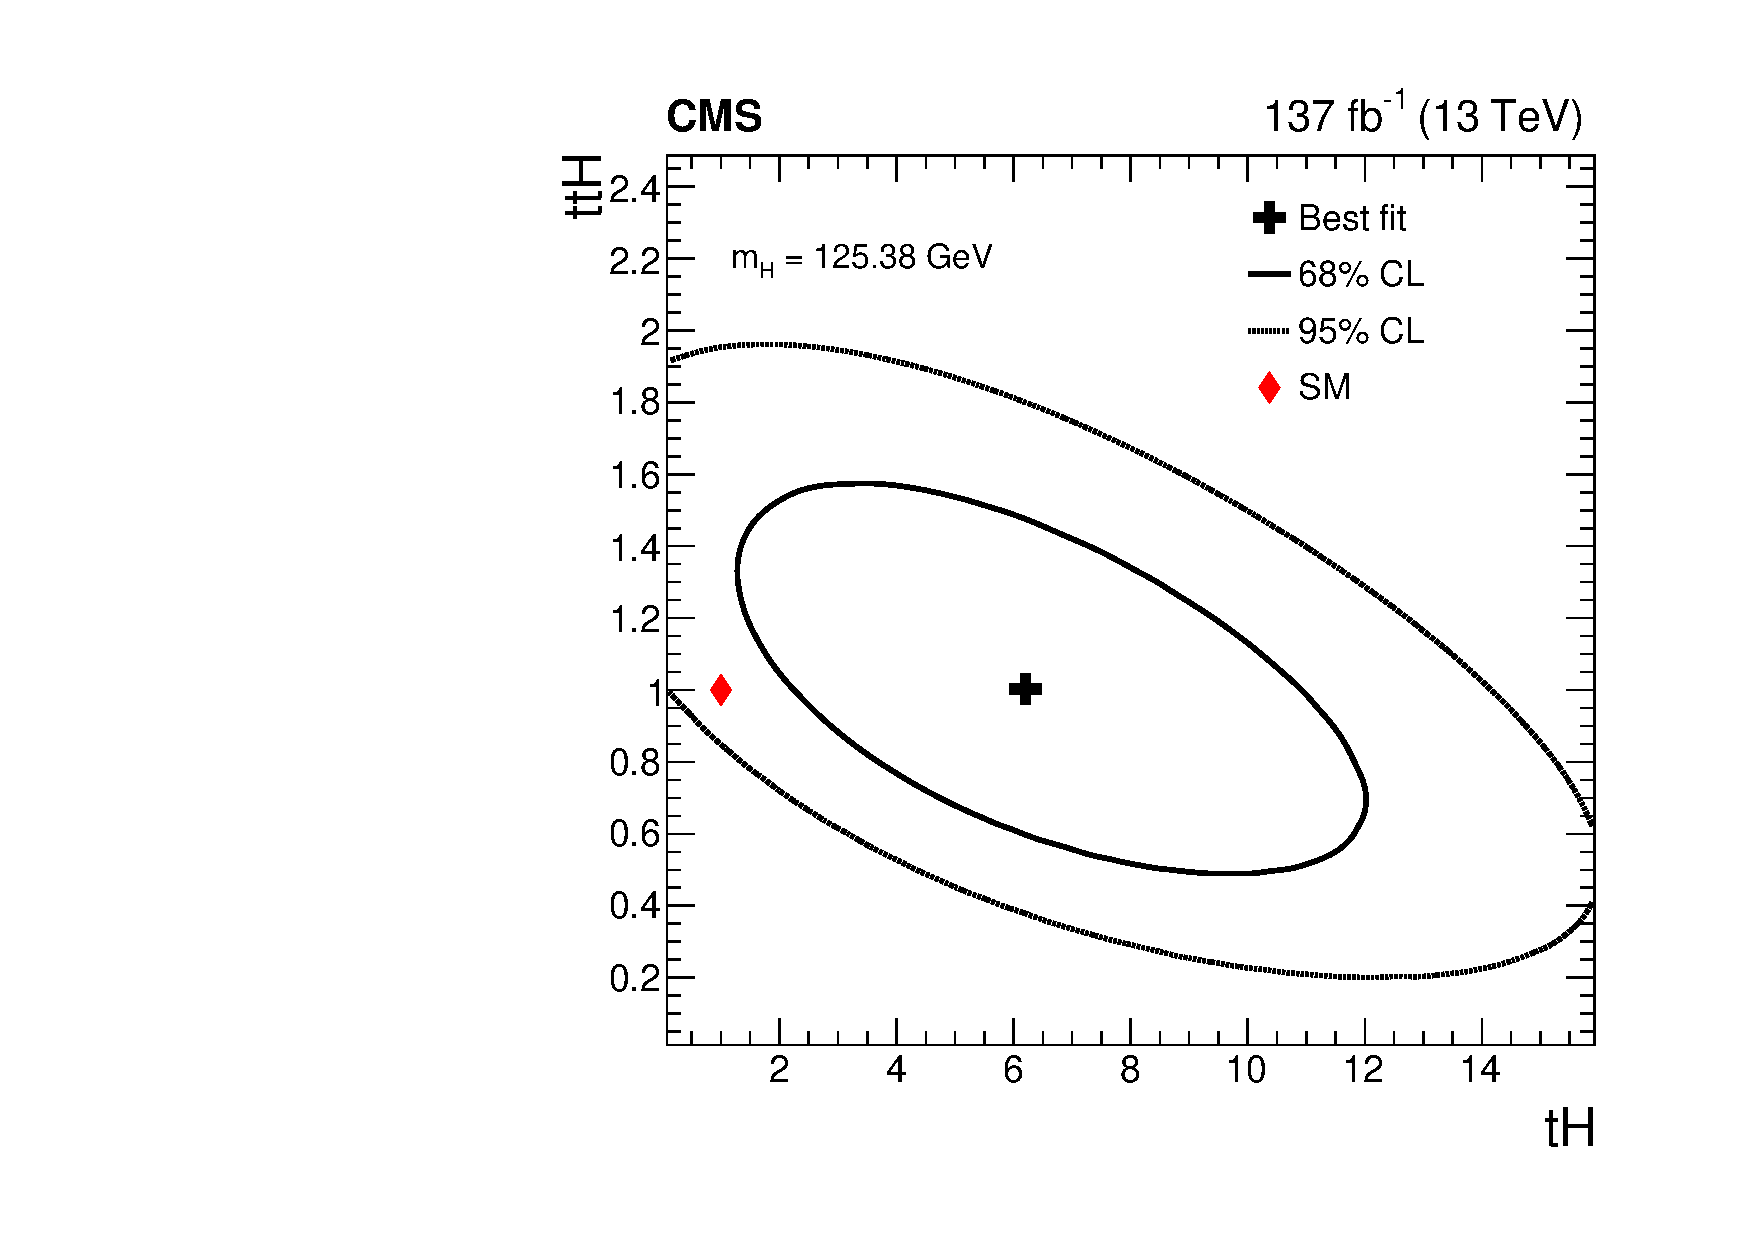
\includegraphics[width=.4\textwidth]{Figures/hgg_results/scan2D_r_tH_vs_r_ttH_obs.pdf}
  \caption[Two dimensional likelihood scans for highly-correlated parameters in the maximal merging scheme]
  {
    Two dimensional $q(\vec{\alpha})$ surfaces for the pairs of parameters in the maximal merging scheme with the largest correlations: ggH VBF-like vs qqH VBF-like (left) and tH vs ttH (right). The best-fit value along with the 68\% and 95\% confidence interval contours are shown by the black cross, solid line and dashed line respectively. The parameters are plotted as a ratio with respect to their SM prediction.
  }
  \label{fig:2d_maximal}
\end{figure}

\begin{table}[htbp]
  \centering
  \scriptsize
  \renewcommand{\arraystretch}{2}
  \setlength{\tabcolsep}{2.2pt}
  \caption[Results of the STXS stage 1.2 maximal merging fit]
  {
    The best-fit cross sections with 68\% confidence intervals for the STXS maximal merging fit. The uncertainty is decomposed into the systematic and statistical components. The expected uncertainties in the fitted parameters are given in brackets. Also listed are the SM predictions for the cross sections times branching fraction and the theoretical uncertainty in these predictions. The final column shows the ratio of the observed value to the SM prediction.
  }
  \label{tab:stage1p2_maximal_results}
  \hspace*{-1cm}
  \begin{tabular}{cccccc}
\multirow{3}{*}{Parameters} & \multicolumn{4}{c}{$\sigma\mathcal{B}$~(fb)} & $\sigma\mathcal{B}$/$(\sigma\mathcal{B})_{\text{SM}}$ \\ 
& SM prediction & \multicolumn{3}{c}{Observed (Expected)} & Observed (Expected) \\ 
& ($\mH=125.38\GeV$) & Best fit & Stat. unc. & Syst. unc. & Best fit \\ \hline 
    ggH 0J low $\ptH$ & \begin{tabular}{r@{}l}$15.21$ & {}$^{+4.14}_{-4.18}$\end{tabular} & \begin{tabular}{r@{}l@{}l}$9.41$ & {}$^{+3.92}_{-3.99}$ & $\Big($$^{+4.20}_{-4.06}$$\Big)$ \end{tabular} & \begin{tabular}{@{}l@{}l}{}$^{+3.90}_{-3.98}$ & $\Big($$^{+4.16}_{-4.05}$$\Big)$ \end{tabular} & \begin{tabular}{@{}l@{}l}{}$^{+0.44}_{-0.25}$ & $\Big($$^{+0.51}_{-0.33}$$\Big)$ \end{tabular} & \begin{tabular}{r@{}l@{}l}$0.62$ & {}$^{+0.26}_{-0.26}$ & $\Big($$^{+0.28}_{-0.27}$$\Big)$ \end{tabular} \\ 
    ggH 0J high $\ptH$ & \begin{tabular}{r@{}l}$44.25$ & {}$^{+4.84}_{-4.61}$\end{tabular} & \begin{tabular}{r@{}l@{}l}$58.50$ & {}$^{+8.10}_{-7.17}$ & $\Big($$^{+7.87}_{-7.77}$$\Big)$ \end{tabular} & \begin{tabular}{@{}l@{}l}{}$^{+7.70}_{-6.91}$ & $\Big($$^{+7.67}_{-7.63}$$\Big)$ \end{tabular} & \begin{tabular}{@{}l@{}l}{}$^{+2.50}_{-1.92}$ & $\Big($$^{+1.78}_{-1.42}$$\Big)$ \end{tabular} & \begin{tabular}{r@{}l@{}l}$1.32$ & {}$^{+0.18}_{-0.16}$ & $\Big($$^{+0.18}_{-0.18}$$\Big)$ \end{tabular} \\ 
    ggH 1J low $\ptH$ & \begin{tabular}{r@{}l}$16.20$ & {}$^{+2.25}_{-2.27}$\end{tabular} & \begin{tabular}{r@{}l@{}l}$13.39$ & {}$^{+5.58}_{-5.49}$ & $\Big($$^{+5.67}_{-5.59}$$\Big)$ \end{tabular} & \begin{tabular}{@{}l@{}l}{}$^{+5.52}_{-5.45}$ & $\Big($$^{+5.61}_{-5.56}$$\Big)$ \end{tabular} & \begin{tabular}{@{}l@{}l}{}$^{+0.80}_{-0.63}$ & $\Big($$^{+0.77}_{-0.48}$$\Big)$ \end{tabular} & \begin{tabular}{r@{}l@{}l}$0.83$ & {}$^{+0.34}_{-0.34}$ & $\Big($$^{+0.35}_{-0.34}$$\Big)$ \end{tabular} \\ 
    ggH 1J med $\ptH$ & \begin{tabular}{r@{}l}$11.23$ & {}$^{+1.56}_{-1.55}$\end{tabular} & \begin{tabular}{r@{}l@{}l}$13.66$ & {}$^{+2.91}_{-2.96}$ & $\Big($$^{+3.15}_{-3.39}$$\Big)$ \end{tabular} & \begin{tabular}{@{}l@{}l}{}$^{+2.83}_{-2.92}$ & $\Big($$^{+3.09}_{-3.36}$$\Big)$ \end{tabular} & \begin{tabular}{@{}l@{}l}{}$^{+0.70}_{-0.50}$ & $\Big($$^{+0.59}_{-0.45}$$\Big)$ \end{tabular} & \begin{tabular}{r@{}l@{}l}$1.22$ & {}$^{+0.26}_{-0.26}$ & $\Big($$^{+0.28}_{-0.30}$$\Big)$ \end{tabular} \\ 
    ggH 1J high $\ptH$ & \begin{tabular}{r@{}l}$2.00$ & {}$^{+0.36}_{-0.36}$\end{tabular} & \begin{tabular}{r@{}l@{}l}$2.56$ & {}$^{+0.90}_{-0.87}$ & $\Big($$^{+0.91}_{-0.92}$$\Big)$ \end{tabular} & \begin{tabular}{@{}l@{}l}{}$^{+0.90}_{-0.87}$ & $\Big($$^{+0.90}_{-0.90}$$\Big)$ \end{tabular} & \begin{tabular}{@{}l@{}l}{}$^{+0.11}_{-0.11}$ & $\Big($$^{+0.15}_{-0.19}$$\Big)$ \end{tabular} & \begin{tabular}{r@{}l@{}l}$1.28$ & {}$^{+0.45}_{-0.44}$ & $\Big($$^{+0.46}_{-0.46}$$\Big)$ \end{tabular} \\ 
    ggH $\geq$2J low $\ptH$ & \begin{tabular}{r@{}l}$2.82$ & {}$^{+0.68}_{-0.68}$\end{tabular} & \begin{tabular}{r@{}l@{}l}$3.62$ & {}$^{+3.65}_{-3.55}$ & $\Big($$^{+3.73}_{-2.82}$$\Big)$ \end{tabular} & \begin{tabular}{@{}l@{}l}{}$^{+3.62}_{-3.53}$ & $\Big($$^{+3.69}_{-2.82}$$\Big)$ \end{tabular} & \begin{tabular}{@{}l@{}l}{}$^{+0.41}_{-0.31}$ & $\Big($$^{+0.55}_{-0.55}$$\Big)$ \end{tabular} & \begin{tabular}{r@{}l@{}l}$1.29$ & {}$^{+1.29}_{-1.26}$ & $\Big($$^{+1.32}_{-1.00}$$\Big)$ \end{tabular} \\ 
    ggH $\geq$2J med $\ptH$ & \begin{tabular}{r@{}l}$4.53$ & {}$^{+1.07}_{-1.07}$\end{tabular} & \begin{tabular}{r@{}l@{}l}$0.08$ & {}$^{+2.77}_{-0.08}$ & $\Big($$^{+2.87}_{-2.82}$$\Big)$ \end{tabular} & \begin{tabular}{@{}l@{}l}{}$^{+2.76}_{-0.08}$ & $\Big($$^{+2.84}_{-2.82}$$\Big)$ \end{tabular} & \begin{tabular}{@{}l@{}l}{}$^{+0.28}_{-0.08}$ & $\Big($$^{+0.38}_{-0.14}$$\Big)$ \end{tabular} & \begin{tabular}{r@{}l@{}l}$0.02$ & {}$^{+0.61}_{-0.02}$ & $\Big($$^{+0.63}_{-0.62}$$\Big)$ \end{tabular} \\ 
    ggH $\geq$2J high $\ptH$ & \begin{tabular}{r@{}l}$2.12$ & {}$^{+0.49}_{-0.50}$\end{tabular} & \begin{tabular}{r@{}l@{}l}$0.82$ & {}$^{+0.92}_{-0.82}$ & $\Big($$^{+1.15}_{-1.10}$$\Big)$ \end{tabular} & \begin{tabular}{@{}l@{}l}{}$^{+0.88}_{-0.82}$ & $\Big($$^{+1.11}_{-1.09}$$\Big)$ \end{tabular} & \begin{tabular}{@{}l@{}l}{}$^{+0.26}_{-0.26}$ & $\Big($$^{+0.31}_{-0.14}$$\Big)$ \end{tabular} & \begin{tabular}{r@{}l@{}l}$0.39$ & {}$^{+0.43}_{-0.39}$ & $\Big($$^{+0.54}_{-0.52}$$\Big)$ \end{tabular} \\ 
    ggH VBF-like & \begin{tabular}{r@{}l}$2.22$ & {}$^{+0.52}_{-0.52}$\end{tabular} & \begin{tabular}{r@{}l@{}l}$5.86$ & {}$^{+2.45}_{-2.59}$ & $\Big($$^{+2.90}_{-2.22}$$\Big)$ \end{tabular} & \begin{tabular}{@{}l@{}l}{}$^{+2.27}_{-2.55}$ & $\Big($$^{+2.81}_{-2.22}$$\Big)$ \end{tabular} & \begin{tabular}{@{}l@{}l}{}$^{+0.92}_{-0.48}$ & $\Big($$^{+0.71}_{-0.71}$$\Big)$ \end{tabular} & \begin{tabular}{r@{}l@{}l}$2.64$ & {}$^{+1.10}_{-1.17}$ & $\Big($$^{+1.31}_{-1.00}$$\Big)$ \end{tabular} \\ 
    ggH BSM & \begin{tabular}{r@{}l}$1.43$ & {}$^{+0.36}_{-0.35}$\end{tabular} & \begin{tabular}{r@{}l@{}l}$1.34$ & {}$^{+0.50}_{-0.47}$ & $\Big($$^{+0.59}_{-0.49}$$\Big)$ \end{tabular} & \begin{tabular}{@{}l@{}l}{}$^{+0.49}_{-0.46}$ & $\Big($$^{+0.58}_{-0.49}$$\Big)$ \end{tabular} & \begin{tabular}{@{}l@{}l}{}$^{+0.05}_{-0.09}$ & $\Big($$^{+0.09}_{-0.05}$$\Big)$ \end{tabular} & \begin{tabular}{r@{}l@{}l}$0.94$ & {}$^{+0.35}_{-0.33}$ & $\Big($$^{+0.41}_{-0.35}$$\Big)$ \end{tabular} \\ 
    qqH VBF-like & \begin{tabular}{r@{}l}$2.96$ & {}$^{+0.59}_{-0.59}$\end{tabular} & \begin{tabular}{r@{}l@{}l}$0.49$ & {}$^{+1.44}_{-0.49}$ & $\Big($$^{+1.49}_{-1.53}$$\Big)$ \end{tabular} & \begin{tabular}{@{}l@{}l}{}$^{+1.40}_{-0.49}$ & $\Big($$^{+1.47}_{-1.47}$$\Big)$ \end{tabular} & \begin{tabular}{@{}l@{}l}{}$^{+0.34}_{-0.34}$ & $\Big($$^{+0.25}_{-0.43}$$\Big)$ \end{tabular} & \begin{tabular}{r@{}l@{}l}$0.17$ & {}$^{+0.49}_{-0.17}$ & $\Big($$^{+0.50}_{-0.52}$$\Big)$ \end{tabular} \\ 
    qqH VH-like & \begin{tabular}{r@{}l}$1.22$ & {}$^{+0.05}_{-0.04}$\end{tabular} & \begin{tabular}{r@{}l@{}l}$1.57$ & {}$^{+1.20}_{-1.24}$ & $\Big($$^{+1.15}_{-1.23}$$\Big)$ \end{tabular} & \begin{tabular}{@{}l@{}l}{}$^{+1.19}_{-1.21}$ & $\Big($$^{+1.15}_{-1.23}$$\Big)$ \end{tabular} & \begin{tabular}{@{}l@{}l}{}$^{+0.13}_{-0.26}$ & $\Big($$^{+0.07}_{-0.04}$$\Big)$ \end{tabular} & \begin{tabular}{r@{}l@{}l}$1.29$ & {}$^{+0.98}_{-1.01}$ & $\Big($$^{+0.94}_{-1.01}$$\Big)$ \end{tabular} \\ 
    qqH BSM & \begin{tabular}{r@{}l}$0.37$ & {}$^{+0.03}_{-0.02}$\end{tabular} & \begin{tabular}{r@{}l@{}l}$0.52$ & {}$^{+0.24}_{-0.22}$ & $\Big($$^{+0.26}_{-0.23}$$\Big)$ \end{tabular} & \begin{tabular}{@{}l@{}l}{}$^{+0.24}_{-0.22}$ & $\Big($$^{+0.25}_{-0.23}$$\Big)$ \end{tabular} & \begin{tabular}{@{}l@{}l}{}$^{+0.03}_{-0.01}$ & $\Big($$^{+0.03}_{-0.01}$$\Big)$ \end{tabular} & \begin{tabular}{r@{}l@{}l}$1.42$ & {}$^{+0.65}_{-0.59}$ & $\Big($$^{+0.69}_{-0.62}$$\Big)$ \end{tabular} \\ 
    WH lep & \begin{tabular}{r@{}l}$0.88$ & {}$^{+0.03}_{-0.03}$\end{tabular} & \begin{tabular}{r@{}l@{}l}$1.19$ & {}$^{+0.49}_{-0.44}$ & $\Big($$^{+0.51}_{-0.42}$$\Big)$ \end{tabular} & \begin{tabular}{@{}l@{}l}{}$^{+0.48}_{-0.43}$ & $\Big($$^{+0.50}_{-0.41}$$\Big)$ \end{tabular} & \begin{tabular}{@{}l@{}l}{}$^{+0.07}_{-0.04}$ & $\Big($$^{+0.05}_{-0.05}$$\Big)$ \end{tabular} & \begin{tabular}{r@{}l@{}l}$1.35$ & {}$^{+0.55}_{-0.49}$ & $\Big($$^{+0.57}_{-0.47}$$\Big)$ \end{tabular} \\ 
    ZH lep & \begin{tabular}{r@{}l}$0.54$ & {}$^{+0.03}_{-0.02}$\end{tabular} & \begin{tabular}{r@{}l@{}l}$0.71$ & {}$^{+0.41}_{-0.35}$ & $\Big($$^{+0.42}_{-0.35}$$\Big)$ \end{tabular} & \begin{tabular}{@{}l@{}l}{}$^{+0.40}_{-0.35}$ & $\Big($$^{+0.41}_{-0.35}$$\Big)$ \end{tabular} & \begin{tabular}{@{}l@{}l}{}$^{+0.07}_{-0.03}$ & $\Big($$^{+0.06}_{-0.03}$$\Big)$ \end{tabular} & \begin{tabular}{r@{}l@{}l}$1.32$ & {}$^{+0.76}_{-0.65}$ & $\Big($$^{+0.78}_{-0.65}$$\Big)$ \end{tabular} \\ 
    ttH & \begin{tabular}{r@{}l}$1.13$ & {}$^{+0.08}_{-0.11}$\end{tabular} & \begin{tabular}{r@{}l@{}l}$1.13$ & {}$^{+0.42}_{-0.39}$ & $\Big($$^{+0.42}_{-0.41}$$\Big)$ \end{tabular} & \begin{tabular}{@{}l@{}l}{}$^{+0.42}_{-0.38}$ & $\Big($$^{+0.41}_{-0.40}$$\Big)$ \end{tabular} & \begin{tabular}{@{}l@{}l}{}$^{+0.07}_{-0.07}$ & $\Big($$^{+0.09}_{-0.05}$$\Big)$ \end{tabular} & \begin{tabular}{r@{}l@{}l}$1.00$ & {}$^{+0.37}_{-0.35}$ & $\Big($$^{+0.37}_{-0.36}$$\Big)$ \end{tabular} \\ 
    tH & \begin{tabular}{r@{}l}$0.20$ & {}$^{+0.01}_{-0.03}$\end{tabular} & \begin{tabular}{r@{}l@{}l}$1.27$ & {}$^{+0.76}_{-0.69}$ & $\Big($$^{+0.76}_{-0.20}$$\Big)$ \end{tabular} & \begin{tabular}{@{}l@{}l}{}$^{+0.75}_{-0.68}$ & $\Big($$^{+0.76}_{-0.20}$$\Big)$ \end{tabular} & \begin{tabular}{@{}l@{}l}{}$^{+0.10}_{-0.13}$ & $\Big($$^{+0.08}_{-0.08}$$\Big)$ \end{tabular} & \begin{tabular}{r@{}l@{}l}$6.24$ & {}$^{+3.72}_{-3.37}$ & $\Big($$^{+3.73}_{-1.00}$$\Big)$ \end{tabular} \\ 
\end{tabular}

  \hspace*{-1cm}
\end{table}

\FloatBarrier

\subsection{Minimal merging scheme}
\begin{figure}[htb!]
  \centering
  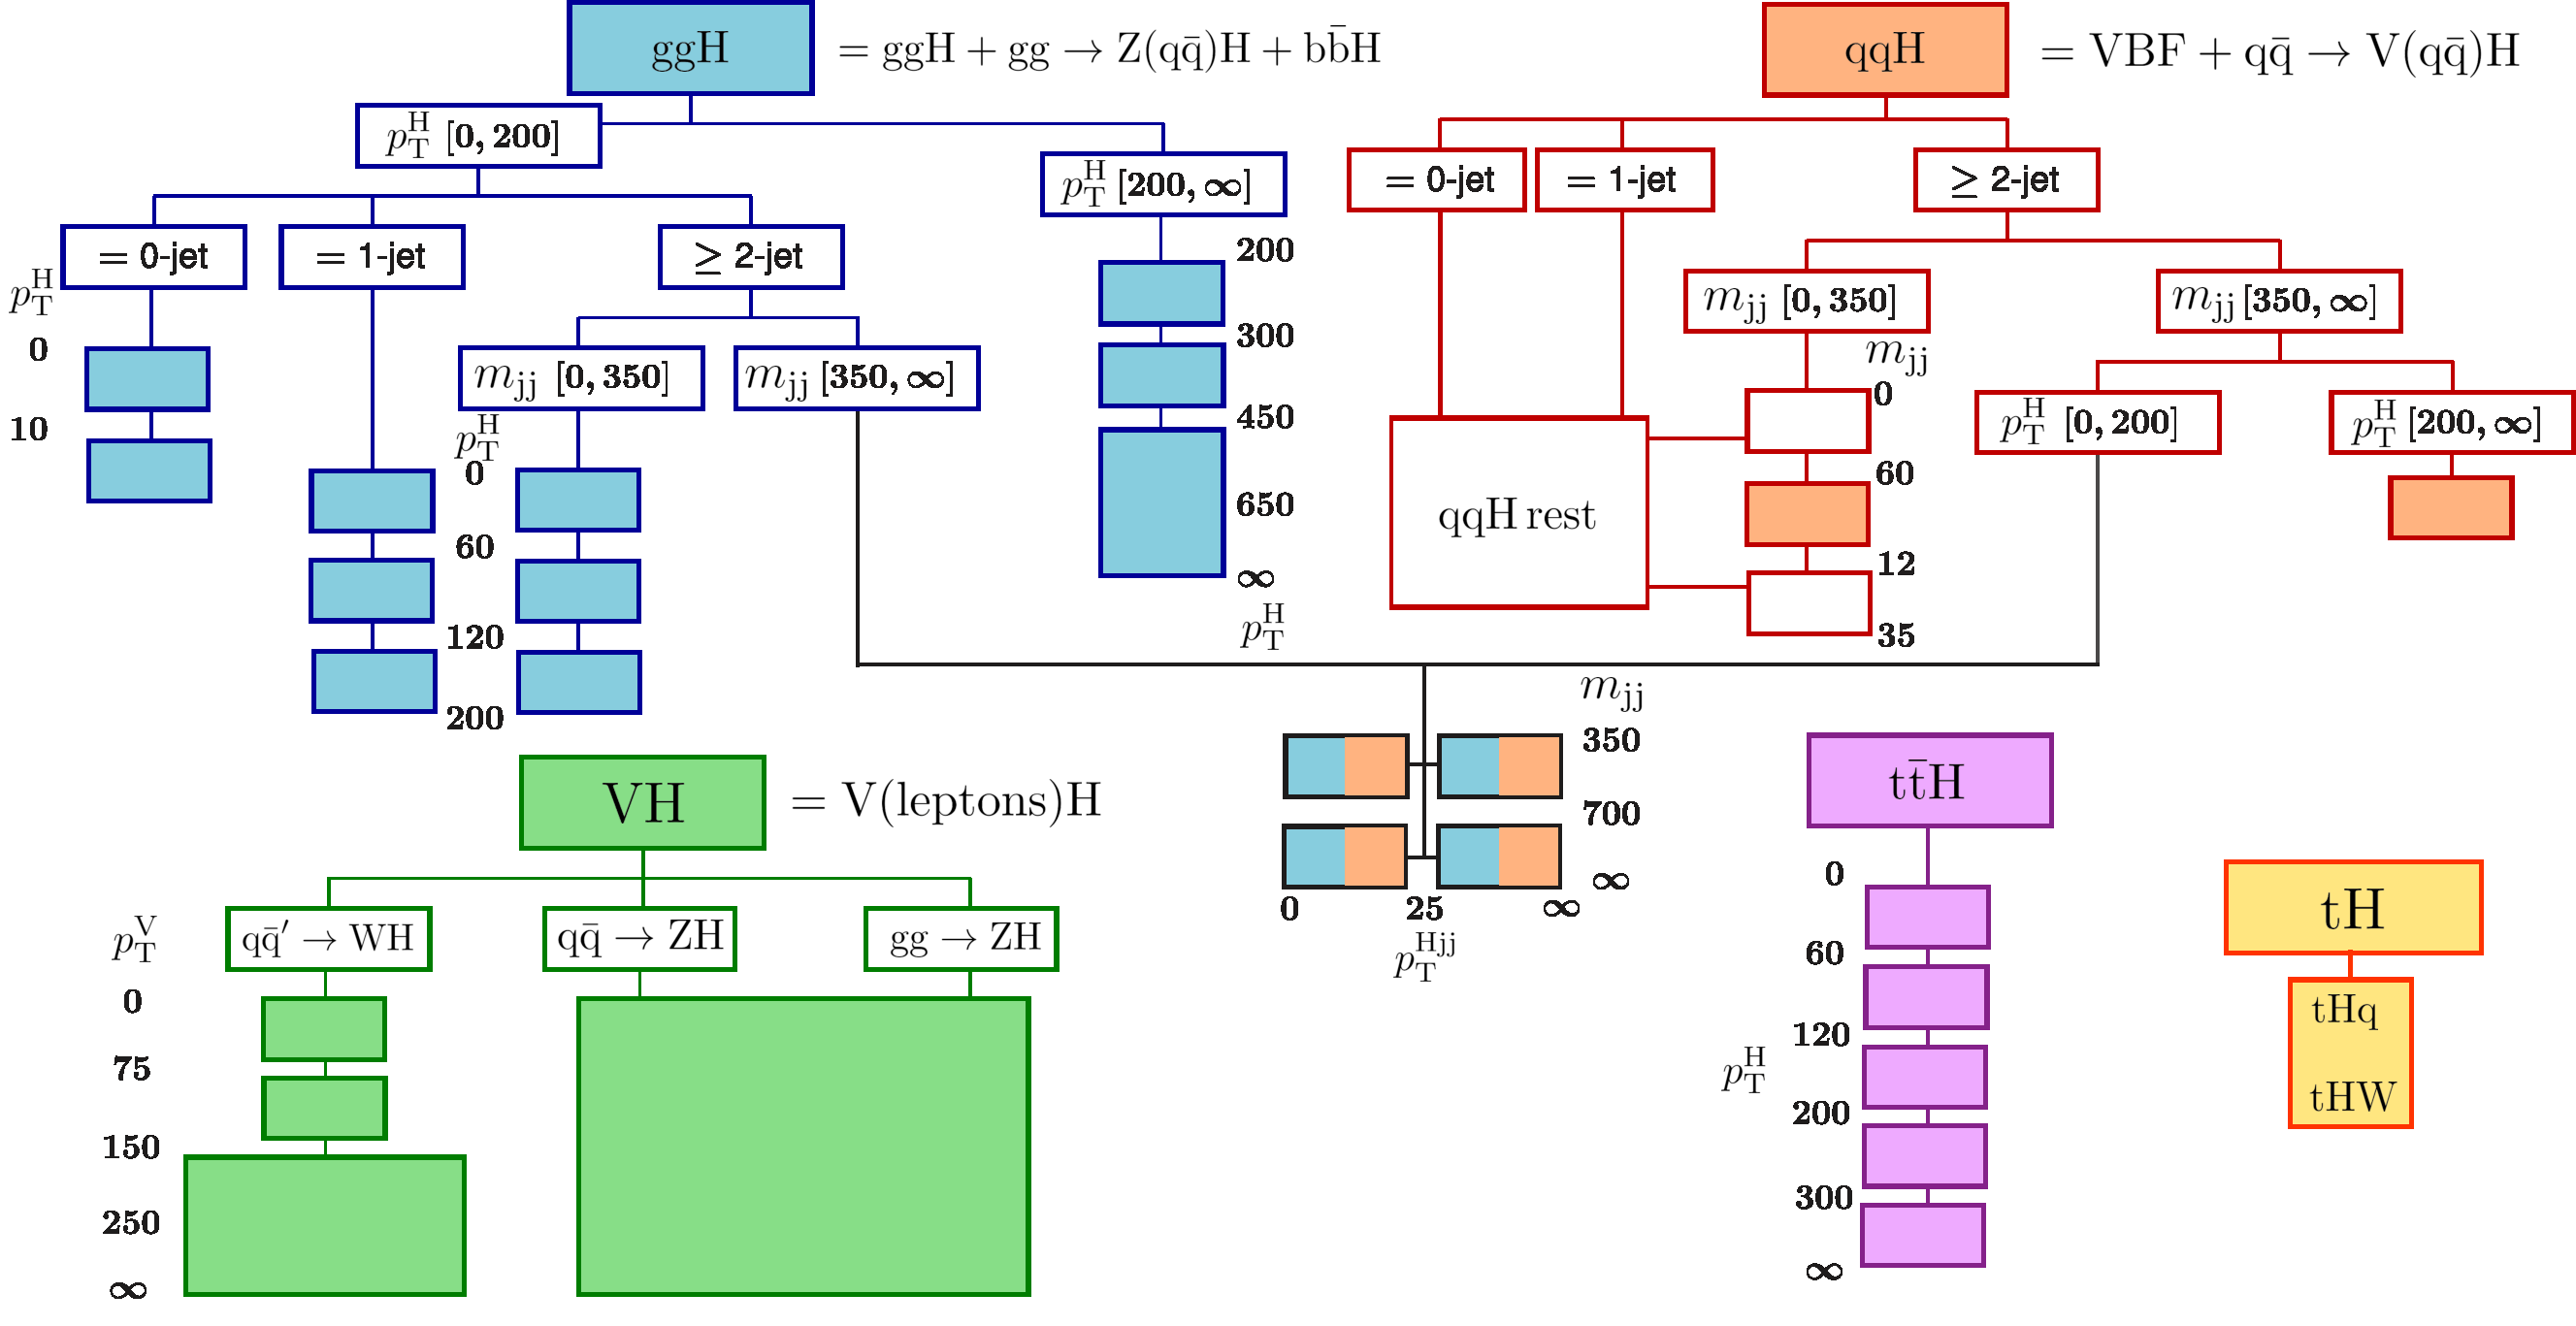
\includegraphics[width=.9\linewidth]{Figures/app_merging_schemes/allSTXSbins_minimal.pdf}
  \caption[Schematic of the minimal merging scheme]
  {
    Schematic to show the minimal merging scheme which defines 27 parameters of interest. Each parameter of interest is shown as a single coloured box.
  }
  \label{fig:minimal_scheme}
\end{figure}

The most granular fit performed in this analysis is in the so-called \textit{minimal merging scheme}. In this scheme a total of 27 parameters of interest are defined, with the aim to merge as few bins as possible whilst ensuring that the correlations between parameters remain smaller than approximately 0.9. In contrast to the maximal scheme, the qqH VBF-like region is fully split into the four STXS bins defined by the boundaries at $\mjj=700$~GeV and $\ptHjj=25$~GeV. To avoid large correlations, the four ggH VBF-like bins are merged with the corresponding bins in the qqH scheme. This approach is more model-independent, as the fit makes no attempt to separate ggH and VBF production in a very similar phase space. Additional splittings are introduced in the ggH scheme at $\ptH=300$~and~450~GeV, and the WH leptonic scheme at $\ptV=75$~and~150~GeV. Furthermore, the ttH region is fully split into five parameters according to the boundaries at $\ptH=60$, 120, 200 and 300~GeV. Again the 0J, 1J, $\mjj<60$ and $120<\mjj<350$ bins in the qqH binning scheme are constrained to their SM prediction within theory uncertainties. The full list of STXS bins which contribute to each parameter are provided in Appendix~\ref{app:merging_table}, with the respective schematic for the minimal merging scheme shown in Figure~\ref{fig:minimal_scheme}.

The \xsbr best-fit values and 68\% confidence intervals in the minimal merging fit are shown in Figure~\ref{fig:stage1p2_minimal_results}, and are listed in Table~\ref{tab:stage1p2_minimal_results}. This result represents the most granular STXS measurement performed by the CMS experiment to-date, showing reasonable sensitivity to many different kinematic regions of Higgs boson production phase space. In particular, the result contains the first measurements of ttH production in different bins, where the size of the uncertainty in each of the four bins with $\ptH<300$~GeV is less than 100\% of the SM prediction. Since the uncertainties in all measured parameters are dominated by the statistical component, there is considerable room for improvement by taking more data and combining with the results from other Higgs boson decay channels. Ultimately, this divide-and-measure approach of the STXS framework allows to systematically constrain increasingly granular regions of phase space, providing sensitivity to BSM physics which may appear in specific kinematic bins. The results here are highly compatible with the SM hypothesis, with a corresponding $p$-value of $p_{\rm{SM}}=70\%$.

\begin{figure}[htb!]
  \centering
  \hspace*{-1.3cm}
  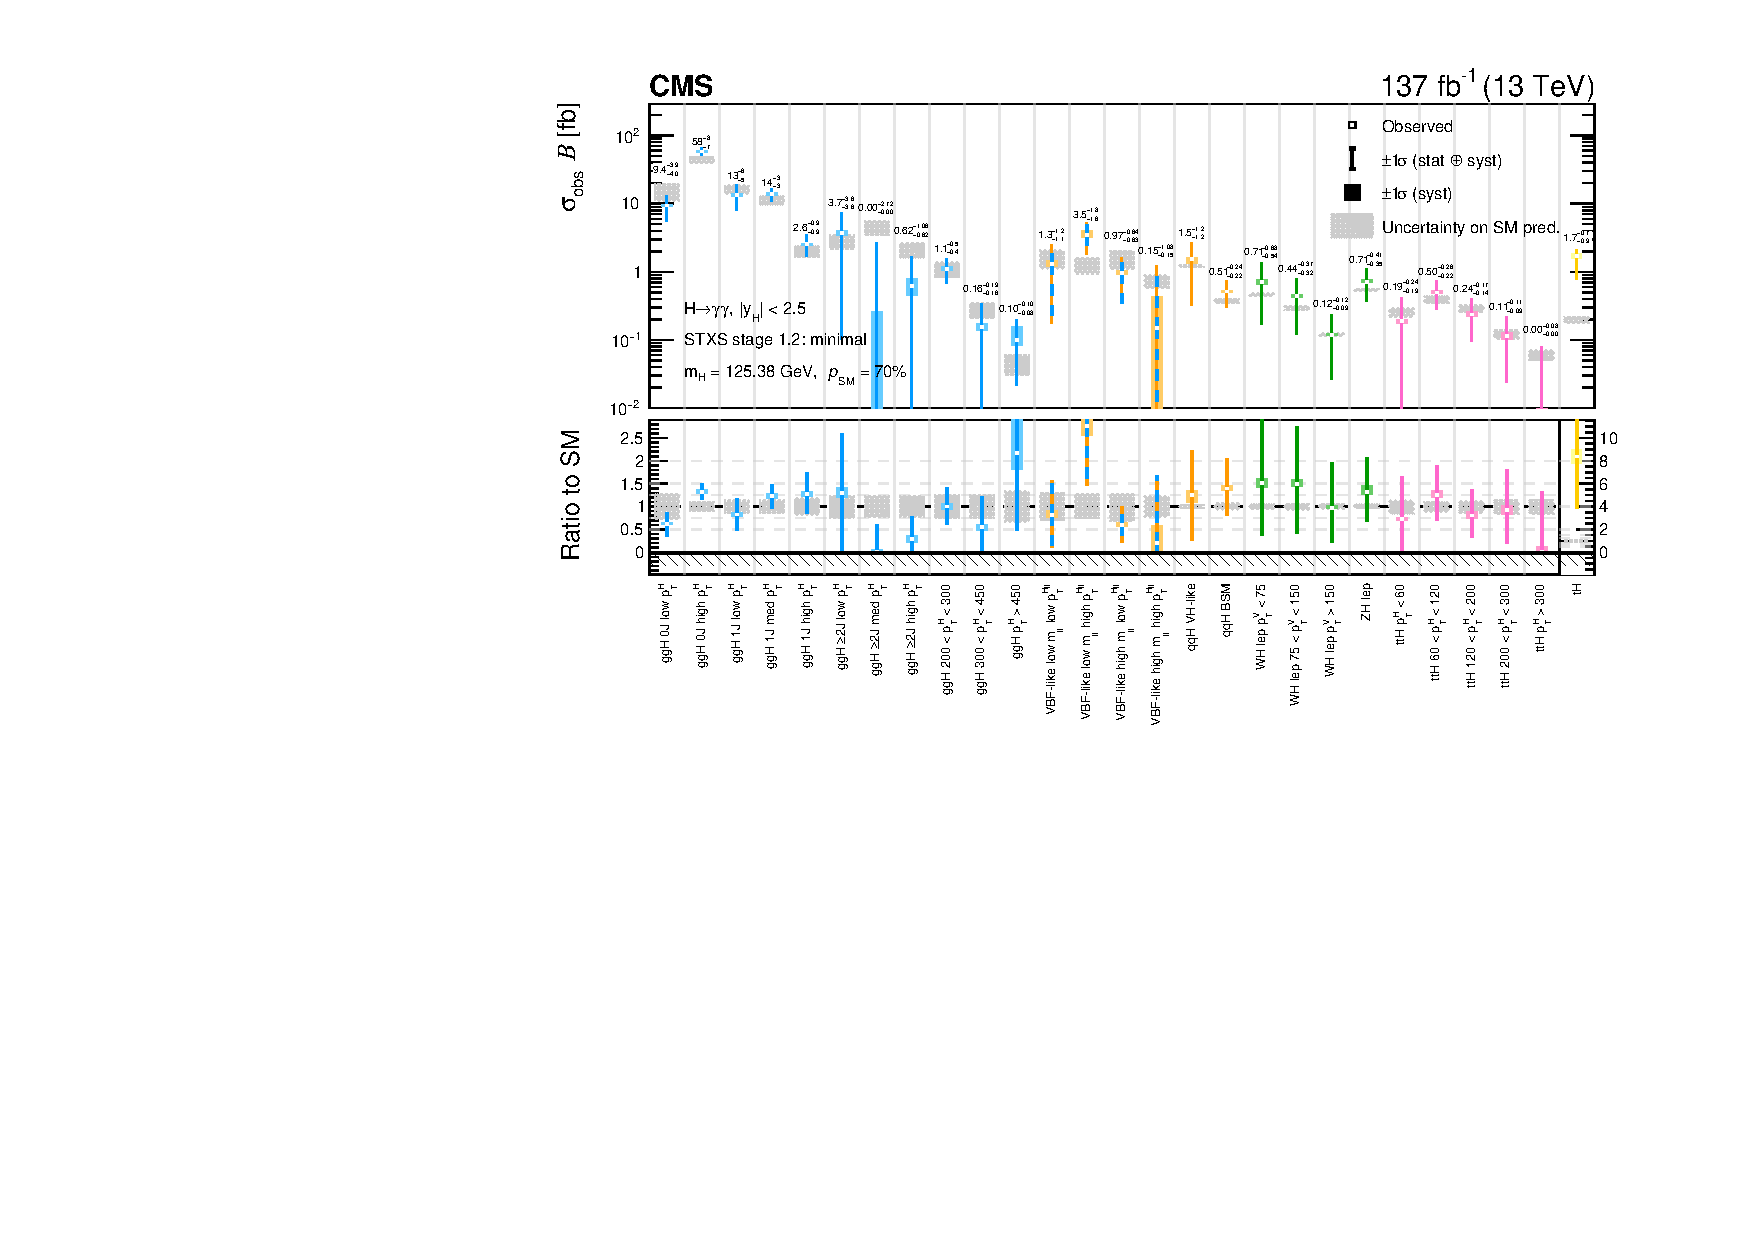
\includegraphics[width=1.2\textwidth]{Figures/hgg_results/stage1p2_minimal_summary.pdf}
  \hspace*{-1.3cm}
  \caption[Results of the STXS stage 1.2 minimal merging fit]
  {
    Observed results of the STXS stage 1.2 minimal merging fit. The best fit cross sections times branching fraction are plotted along with the respective 68\% confidence intervals. The systematic components of the uncertainty in each parameter are shown by the coloured boxes. The hatched grey boxes represent the theoretical uncertainty in the SM predictions. The bottom panel shows the ratio of the fitted values to the SM predictions. The colour scheme has been chosen to match the STXS schematic in Figure \ref{fig:stxs_schematic}, such that the orange and blue dashed line for the VBF-like parameters represents the contributions from both ggH and qqH STXS bins. The compatibility of this fit with the SM prediction is approximately $p_{\rm{SM}}=70\%$. 
  }
  \label{fig:stage1p2_minimal_results}
\end{figure}

The correlations between parameters are shown in Figure~\ref{fig:stage1p2_minimal_correlations}. By merging the qqH VBF-like STXS bins with the equivalent bins in the ggH scheme, the correlations in this region of phase space are kept to an acceptable level. The region with the highest correlations is that defined by the high \ptH ttH and tH parameters. With such high correlations, the act of splitting ttH into five separate parameters forces the tH \xsbr to an even higher value, corresponding to an excess of approximately eight times the SM prediction. 

% Finally, the observed diphoton mass distributions are shown for all eighty analysis categories in Appendix~\ref{app:massfits}. The signal-plus-background model displayed in the plots corresponds to the best-fit model in the minimal merging scheme i.e. the signal parametrisation with the most degrees of freedom considered in this analysis.

\begin{figure}[htb!]
  \centering
  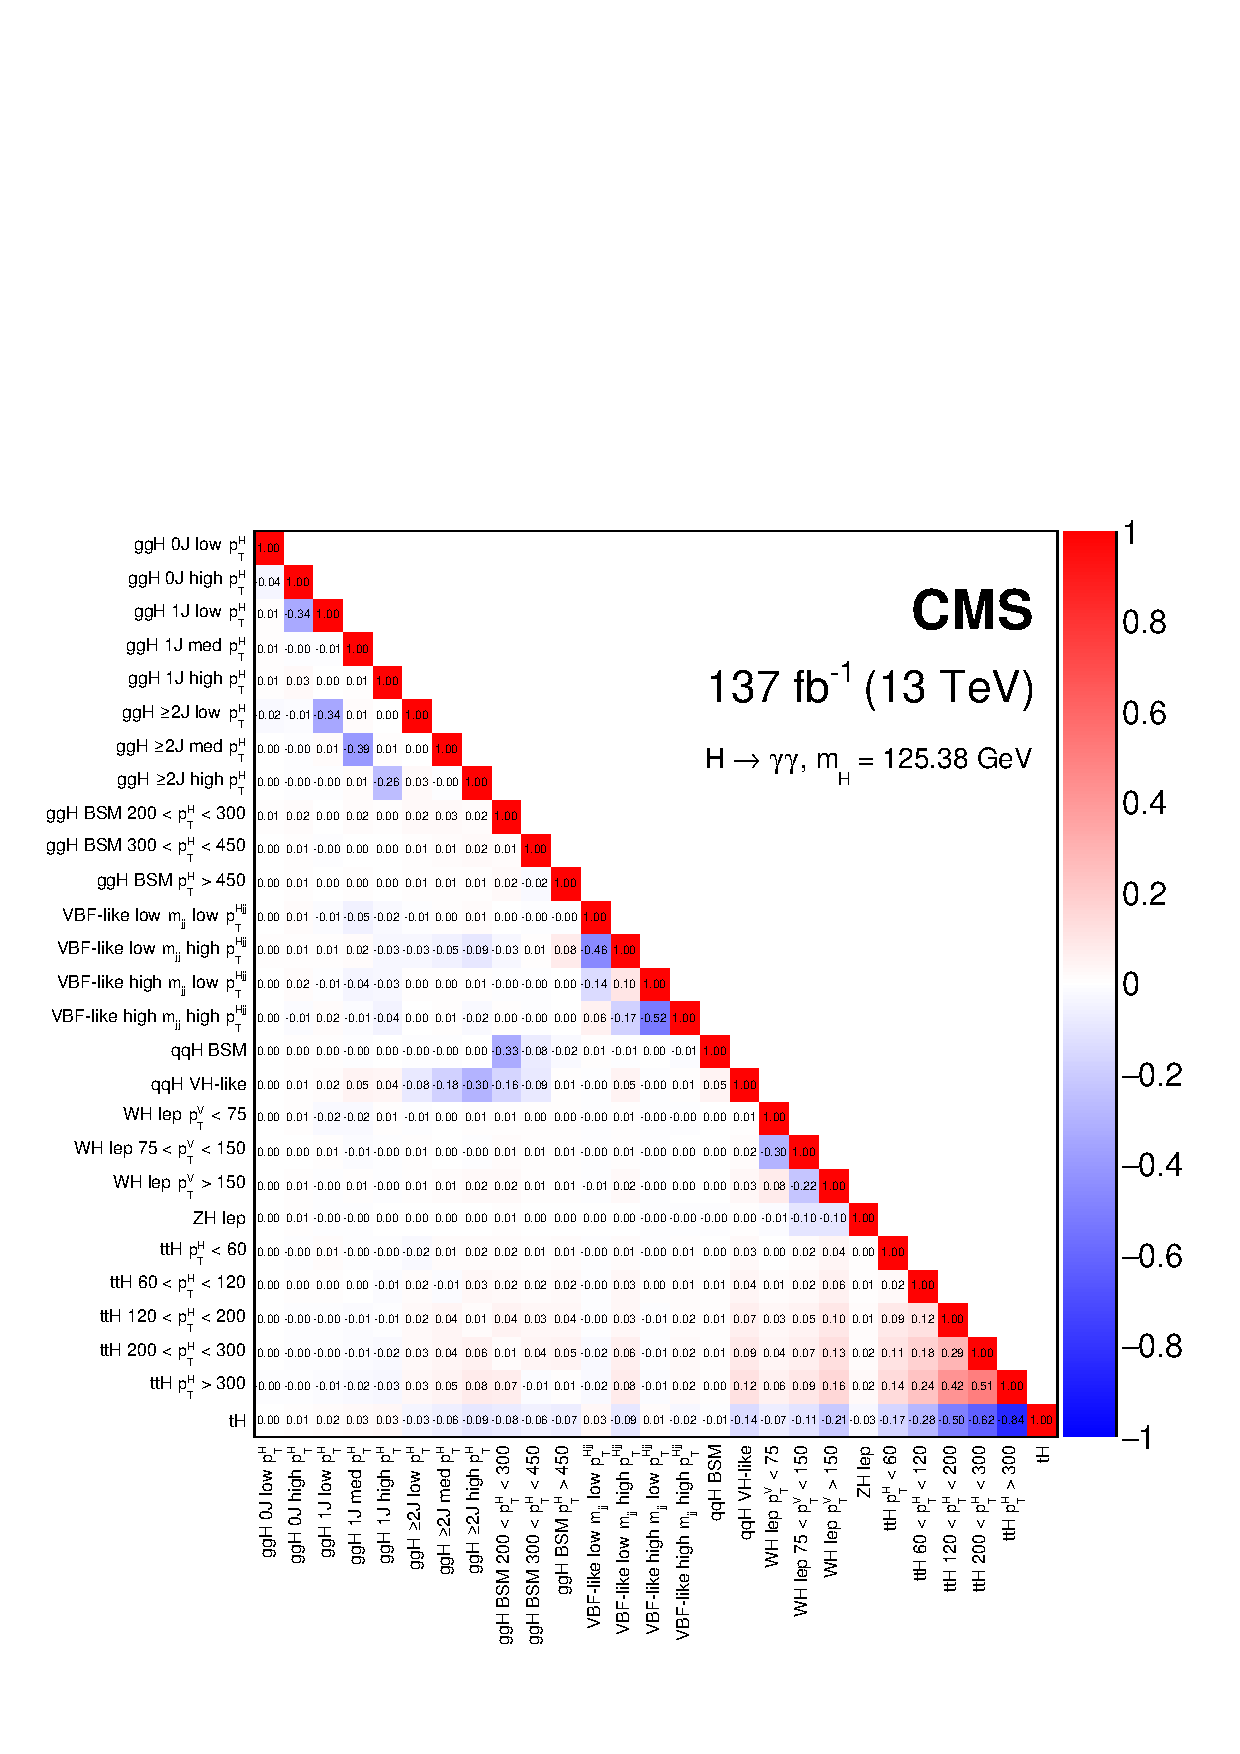
\includegraphics[width=.93\textwidth]{Figures/hgg_results/stage1p2_minimal_correlations.pdf}
  \caption[Correlations in the STXS stage 1.2 minimal merging parameters]
  {
    Observed correlations between the 27 parameters in the STXS stage 1.2 minimal merging fit. The size of the correlations is indicated by the colour scale.
  }
  \label{fig:stage1p2_minimal_correlations}
\end{figure}

\begin{table}[htb!]
  \centering
  \scriptsize
  \renewcommand{\arraystretch}{1.8}
  \setlength{\tabcolsep}{2.2pt}
  \caption[Results of the STXS stage 1.2 minimal merging fit]
  {
    The best-fit cross sections with 68\% confidence intervals for the STXS minimal merging fit. The uncertainty is decomposed into the systematic and statistical components. The expected uncertainties in the fitted parameters are given in brackets. Also listed are the SM predictions for the cross sections times branching fraction and the theoretical uncertainty in these predictions. The final column shows the ratio of the observed value to the SM prediction.
  }
  \label{tab:stage1p2_minimal_results}
  \hspace*{-.5cm}
  \begin{tabular}{cccccc}
    \multirow{3}{*}{Parameters} & \multicolumn{4}{c}{$\sigma\mathcal{B}$~(fb)} & $\sigma\mathcal{B}$/$(\sigma\mathcal{B})_{\text{SM}}$ \\ 
    & SM prediction & \multicolumn{3}{c}{Observed (Expected)} & Observed (Expected) \\ 
    & ($\mH=125.38\GeV$) & Best fit & Stat. unc. & Syst. unc. & Best fit \\ \hline 
    ggH 0J low $\ptH$ & \begin{tabular}{r@{}l}$15.21$ & {}$^{+4.14}_{-4.18}$\end{tabular} & \begin{tabular}{r@{}l@{}l}$9.41$ & {}$^{+3.91}_{-4.00}$ & $\Big($$^{+4.19}_{-4.06}$$\Big)$ \end{tabular} & \begin{tabular}{@{}l@{}l}{}$^{+3.90}_{-3.99}$ & $\Big($$^{+4.16}_{-4.05}$$\Big)$ \end{tabular} & \begin{tabular}{@{}l@{}l}{}$^{+0.37}_{-0.30}$ & $\Big($$^{+0.50}_{-0.36}$$\Big)$ \end{tabular} & \begin{tabular}{r@{}l@{}l}$0.62$ & {}$^{+0.26}_{-0.26}$ & $\Big($$^{+0.28}_{-0.27}$$\Big)$ \end{tabular} \\ 
    ggH 0J high $\ptH$ & \begin{tabular}{r@{}l}$44.25$ & {}$^{+4.84}_{-4.61}$\end{tabular} & \begin{tabular}{r@{}l@{}l}$58.46$ & {}$^{+8.12}_{-7.17}$ & $\Big($$^{+7.87}_{-7.78}$$\Big)$ \end{tabular} & \begin{tabular}{@{}l@{}l}{}$^{+7.69}_{-6.91}$ & $\Big($$^{+7.66}_{-7.63}$$\Big)$ \end{tabular} & \begin{tabular}{@{}l@{}l}{}$^{+2.60}_{-1.94}$ & $\Big($$^{+1.78}_{-1.50}$$\Big)$ \end{tabular} & \begin{tabular}{r@{}l@{}l}$1.32$ & {}$^{+0.18}_{-0.16}$ & $\Big($$^{+0.18}_{-0.18}$$\Big)$ \end{tabular} \\ 
    ggH 1J low $\ptH$ & \begin{tabular}{r@{}l}$16.20$ & {}$^{+2.25}_{-2.27}$\end{tabular} & \begin{tabular}{r@{}l@{}l}$13.40$ & {}$^{+5.59}_{-5.50}$ & $\Big($$^{+5.70}_{-5.58}$$\Big)$ \end{tabular} & \begin{tabular}{@{}l@{}l}{}$^{+5.53}_{-5.46}$ & $\Big($$^{+5.64}_{-5.55}$$\Big)$ \end{tabular} & \begin{tabular}{@{}l@{}l}{}$^{+0.79}_{-0.67}$ & $\Big($$^{+0.77}_{-0.56}$$\Big)$ \end{tabular} & \begin{tabular}{r@{}l@{}l}$0.83$ & {}$^{+0.34}_{-0.34}$ & $\Big($$^{+0.35}_{-0.34}$$\Big)$ \end{tabular} \\ 
    ggH 1J med $\ptH$ & \begin{tabular}{r@{}l}$11.23$ & {}$^{+1.56}_{-1.55}$\end{tabular} & \begin{tabular}{r@{}l@{}l}$13.80$ & {}$^{+2.90}_{-2.94}$ & $\Big($$^{+3.14}_{-3.41}$$\Big)$ \end{tabular} & \begin{tabular}{@{}l@{}l}{}$^{+2.82}_{-2.90}$ & $\Big($$^{+3.08}_{-3.37}$$\Big)$ \end{tabular} & \begin{tabular}{@{}l@{}l}{}$^{+0.68}_{-0.51}$ & $\Big($$^{+0.59}_{-0.50}$$\Big)$ \end{tabular} & \begin{tabular}{r@{}l@{}l}$1.23$ & {}$^{+0.26}_{-0.26}$ & $\Big($$^{+0.28}_{-0.30}$$\Big)$ \end{tabular} \\ 
    ggH 1J high $\ptH$ & \begin{tabular}{r@{}l}$2.00$ & {}$^{+0.36}_{-0.36}$\end{tabular} & \begin{tabular}{r@{}l@{}l}$2.57$ & {}$^{+0.94}_{-0.88}$ & $\Big($$^{+0.92}_{-0.90}$$\Big)$ \end{tabular} & \begin{tabular}{@{}l@{}l}{}$^{+0.94}_{-0.87}$ & $\Big($$^{+0.91}_{-0.88}$$\Big)$ \end{tabular} & \begin{tabular}{@{}l@{}l}{}$^{+0.08}_{-0.12}$ & $\Big($$^{+0.13}_{-0.16}$$\Big)$ \end{tabular} & \begin{tabular}{r@{}l@{}l}$1.28$ & {}$^{+0.47}_{-0.44}$ & $\Big($$^{+0.46}_{-0.45}$$\Big)$ \end{tabular} \\ 
    ggH $\geq2$J low $\ptH$ & \begin{tabular}{r@{}l}$2.82$ & {}$^{+0.68}_{-0.68}$\end{tabular} & \begin{tabular}{r@{}l@{}l}$3.67$ & {}$^{+3.63}_{-3.57}$ & $\Big($$^{+3.74}_{-2.82}$$\Big)$ \end{tabular} & \begin{tabular}{@{}l@{}l}{}$^{+3.62}_{-3.56}$ & $\Big($$^{+3.71}_{-2.82}$$\Big)$ \end{tabular} & \begin{tabular}{@{}l@{}l}{}$^{+0.34}_{-0.30}$ & $\Big($$^{+0.49}_{-0.49}$$\Big)$ \end{tabular} & \begin{tabular}{r@{}l@{}l}$1.30$ & {}$^{+1.29}_{-1.27}$ & $\Big($$^{+1.33}_{-1.00}$$\Big)$ \end{tabular} \\ 
    ggH $\geq2$J med $\ptH$ & \begin{tabular}{r@{}l}$4.53$ & {}$^{+1.07}_{-1.07}$\end{tabular} & \begin{tabular}{r@{}l@{}l}$0.00$ & {}$^{+2.72}_{-0.00}$ & $\Big($$^{+2.90}_{-2.80}$$\Big)$ \end{tabular} & \begin{tabular}{@{}l@{}l}{}$^{+2.71}_{-0.00}$ & $\Big($$^{+2.86}_{-2.78}$$\Big)$ \end{tabular} & \begin{tabular}{@{}l@{}l}{}$^{+0.26}_{-0.00}$ & $\Big($$^{+0.45}_{-0.27}$$\Big)$ \end{tabular} & \begin{tabular}{r@{}l@{}l}$0.00$ & {}$^{+0.60}_{-0.00}$ & $\Big($$^{+0.64}_{-0.62}$$\Big)$ \end{tabular} \\ 
    ggH $\geq2$J high $\ptH$ & \begin{tabular}{r@{}l}$2.12$ & {}$^{+0.49}_{-0.50}$\end{tabular} & \begin{tabular}{r@{}l@{}l}$0.62$ & {}$^{+1.06}_{-0.62}$ & $\Big($$^{+1.15}_{-1.10}$$\Big)$ \end{tabular} & \begin{tabular}{@{}l@{}l}{}$^{+1.04}_{-0.62}$ & $\Big($$^{+1.11}_{-1.10}$$\Big)$ \end{tabular} & \begin{tabular}{@{}l@{}l}{}$^{+0.17}_{-0.17}$ & $\Big($$^{+0.30}_{-0.13}$$\Big)$ \end{tabular} & \begin{tabular}{r@{}l@{}l}$0.29$ & {}$^{+0.50}_{-0.29}$ & $\Big($$^{+0.54}_{-0.52}$$\Big)$ \end{tabular} \\ 
    ggH BSM $200<\ptH<300$ & \begin{tabular}{r@{}l}$1.10$ & {}$^{+0.28}_{-0.27}$\end{tabular} & \begin{tabular}{r@{}l@{}l}$1.11$ & {}$^{+0.47}_{-0.44}$ & $\Big($$^{+0.56}_{-0.45}$$\Big)$ \end{tabular} & \begin{tabular}{@{}l@{}l}{}$^{+0.46}_{-0.43}$ & $\Big($$^{+0.56}_{-0.45}$$\Big)$ \end{tabular} & \begin{tabular}{@{}l@{}l}{}$^{+0.08}_{-0.07}$ & $\Big($$^{+0.05}_{-0.03}$$\Big)$ \end{tabular} & \begin{tabular}{r@{}l@{}l}$1.00$ & {}$^{+0.42}_{-0.40}$ & $\Big($$^{+0.51}_{-0.41}$$\Big)$ \end{tabular} \\ 
    ggH BSM $300<\ptH<450$ & \begin{tabular}{r@{}l}$0.28$ & {}$^{+0.07}_{-0.07}$\end{tabular} & \begin{tabular}{r@{}l@{}l}$0.16$ & {}$^{+0.19}_{-0.16}$ & $\Big($$^{+0.20}_{-0.18}$$\Big)$ \end{tabular} & \begin{tabular}{@{}l@{}l}{}$^{+0.18}_{-0.16}$ & $\Big($$^{+0.19}_{-0.18}$$\Big)$ \end{tabular} & \begin{tabular}{@{}l@{}l}{}$^{+0.02}_{-0.02}$ & $\Big($$^{+0.03}_{-0.01}$$\Big)$ \end{tabular} & \begin{tabular}{r@{}l@{}l}$0.55$ & {}$^{+0.66}_{-0.55}$ & $\Big($$^{+0.69}_{-0.65}$$\Big)$ \end{tabular} \\ 
    ggH BSM $\ptH>450$ & \begin{tabular}{r@{}l}$0.05$ & {}$^{+0.02}_{-0.02}$\end{tabular} & \begin{tabular}{r@{}l@{}l}$0.10$ & {}$^{+0.10}_{-0.08}$ & $\Big($$^{+0.10}_{-0.05}$$\Big)$ \end{tabular} & \begin{tabular}{@{}l@{}l}{}$^{+0.09}_{-0.08}$ & $\Big($$^{+0.09}_{-0.05}$$\Big)$ \end{tabular} & \begin{tabular}{@{}l@{}l}{}$^{+0.06}_{-0.02}$ & $\Big($$^{+0.04}_{-0.04}$$\Big)$ \end{tabular} & \begin{tabular}{r@{}l@{}l}$2.16$ & {}$^{+2.25}_{-1.69}$ & $\Big($$^{+2.19}_{-1.00}$$\Big)$ \end{tabular} \\ 
    VBF-like low $\mjj$ low $\ptHjj$ & \begin{tabular}{r@{}l}$1.59$ & {}$^{+0.49}_{-0.48}$\end{tabular} & \begin{tabular}{r@{}l@{}l}$1.31$ & {}$^{+1.19}_{-1.13}$ & $\Big($$^{+1.22}_{-1.16}$$\Big)$ \end{tabular} & \begin{tabular}{@{}l@{}l}{}$^{+1.18}_{-1.13}$ & $\Big($$^{+1.21}_{-1.16}$$\Big)$ \end{tabular} & \begin{tabular}{@{}l@{}l}{}$^{+0.14}_{-0.09}$ & $\Big($$^{+0.13}_{-0.05}$$\Big)$ \end{tabular} & \begin{tabular}{r@{}l@{}l}$0.82$ & {}$^{+0.75}_{-0.71}$ & $\Big($$^{+0.77}_{-0.73}$$\Big)$ \end{tabular} \\ 
    VBF-like low $\mjj$ high $\ptHjj$ & \begin{tabular}{r@{}l}$1.25$ & {}$^{+0.35}_{-0.32}$\end{tabular} & \begin{tabular}{r@{}l@{}l}$3.46$ & {}$^{+1.76}_{-1.64}$ & $\Big($$^{+1.79}_{-1.25}$$\Big)$ \end{tabular} & \begin{tabular}{@{}l@{}l}{}$^{+1.65}_{-1.62}$ & $\Big($$^{+1.76}_{-1.25}$$\Big)$ \end{tabular} & \begin{tabular}{@{}l@{}l}{}$^{+0.61}_{-0.25}$ & $\Big($$^{+0.32}_{-0.32}$$\Big)$ \end{tabular} & \begin{tabular}{r@{}l@{}l}$2.76$ & {}$^{+1.40}_{-1.31}$ & $\Big($$^{+1.43}_{-1.00}$$\Big)$ \end{tabular} \\ 
    VBF-like high $\mjj$ low $\ptHjj$ & \begin{tabular}{r@{}l}$1.60$ & {}$^{+0.45}_{-0.51}$\end{tabular} & \begin{tabular}{r@{}l@{}l}$0.97$ & {}$^{+0.64}_{-0.63}$ & $\Big($$^{+0.72}_{-0.63}$$\Big)$ \end{tabular} & \begin{tabular}{@{}l@{}l}{}$^{+0.63}_{-0.62}$ & $\Big($$^{+0.71}_{-0.63}$$\Big)$ \end{tabular} & \begin{tabular}{@{}l@{}l}{}$^{+0.07}_{-0.07}$ & $\Big($$^{+0.11}_{-0.06}$$\Big)$ \end{tabular} & \begin{tabular}{r@{}l@{}l}$0.61$ & {}$^{+0.40}_{-0.39}$ & $\Big($$^{+0.45}_{-0.39}$$\Big)$ \end{tabular} \\ 
    VBF-like high $\mjj$ high $\ptHjj$ & \begin{tabular}{r@{}l}$0.73$ & {}$^{+0.16}_{-0.16}$\end{tabular} & \begin{tabular}{r@{}l@{}l}$0.15$ & {}$^{+1.08}_{-0.15}$ & $\Big($$^{+0.93}_{-0.73}$$\Big)$ \end{tabular} & \begin{tabular}{@{}l@{}l}{}$^{+1.04}_{-0.15}$ & $\Big($$^{+0.92}_{-0.73}$$\Big)$ \end{tabular} & \begin{tabular}{@{}l@{}l}{}$^{+0.28}_{-0.15}$ & $\Big($$^{+0.14}_{-0.14}$$\Big)$ \end{tabular} & \begin{tabular}{r@{}l@{}l}$0.20$ & {}$^{+1.47}_{-0.20}$ & $\Big($$^{+1.26}_{-1.00}$$\Big)$ \end{tabular} \\ 
    qqH VH-like & \begin{tabular}{r@{}l}$1.22$ & {}$^{+0.05}_{-0.05}$\end{tabular} & \begin{tabular}{r@{}l@{}l}$1.53$ & {}$^{+1.20}_{-1.21}$ & $\Big($$^{+1.13}_{-1.27}$$\Big)$ \end{tabular} & \begin{tabular}{@{}l@{}l}{}$^{+1.20}_{-1.20}$ & $\Big($$^{+1.12}_{-1.27}$$\Big)$ \end{tabular} & \begin{tabular}{@{}l@{}l}{}$^{+0.11}_{-0.19}$ & $\Big($$^{+0.05}_{-0.08}$$\Big)$ \end{tabular} & \begin{tabular}{r@{}l@{}l}$1.25$ & {}$^{+0.98}_{-0.99}$ & $\Big($$^{+0.92}_{-1.04}$$\Big)$ \end{tabular} \\ 
    qqH BSM & \begin{tabular}{r@{}l}$0.37$ & {}$^{+0.03}_{-0.02}$\end{tabular} & \begin{tabular}{r@{}l@{}l}$0.51$ & {}$^{+0.24}_{-0.22}$ & $\Big($$^{+0.24}_{-0.24}$$\Big)$ \end{tabular} & \begin{tabular}{@{}l@{}l}{}$^{+0.24}_{-0.22}$ & $\Big($$^{+0.24}_{-0.24}$$\Big)$ \end{tabular} & \begin{tabular}{@{}l@{}l}{}$^{+0.03}_{-0.01}$ & $\Big($$^{+0.03}_{-0.02}$$\Big)$ \end{tabular} & \begin{tabular}{r@{}l@{}l}$1.40$ & {}$^{+0.66}_{-0.60}$ & $\Big($$^{+0.66}_{-0.65}$$\Big)$ \end{tabular} \\ 
    WH lep $\ptV<75$ & \begin{tabular}{r@{}l}$0.47$ & {}$^{+0.02}_{-0.02}$\end{tabular} & \begin{tabular}{r@{}l@{}l}$0.71$ & {}$^{+0.68}_{-0.54}$ & $\Big($$^{+0.75}_{-0.47}$$\Big)$ \end{tabular} & \begin{tabular}{@{}l@{}l}{}$^{+0.68}_{-0.54}$ & $\Big($$^{+0.75}_{-0.47}$$\Big)$ \end{tabular} & \begin{tabular}{@{}l@{}l}{}$^{+0.05}_{-0.05}$ & $\Big($$^{+0.05}_{-0.05}$$\Big)$ \end{tabular} & \begin{tabular}{r@{}l@{}l}$1.51$ & {}$^{+1.45}_{-1.15}$ & $\Big($$^{+1.60}_{-1.00}$$\Big)$ \end{tabular} \\ 
    WH lep $75<\ptV<150$ & \begin{tabular}{r@{}l}$0.29$ & {}$^{+0.02}_{-0.02}$\end{tabular} & \begin{tabular}{r@{}l@{}l}$0.44$ & {}$^{+0.37}_{-0.32}$ & $\Big($$^{+0.37}_{-0.29}$$\Big)$ \end{tabular} & \begin{tabular}{@{}l@{}l}{}$^{+0.37}_{-0.32}$ & $\Big($$^{+0.37}_{-0.29}$$\Big)$ \end{tabular} & \begin{tabular}{@{}l@{}l}{}$^{+0.03}_{-0.02}$ & $\Big($$^{+0.02}_{-0.02}$$\Big)$ \end{tabular} & \begin{tabular}{r@{}l@{}l}$1.49$ & {}$^{+1.26}_{-1.08}$ & $\Big($$^{+1.25}_{-1.00}$$\Big)$ \end{tabular} \\ 
    WH lep $\ptV>150$ & \begin{tabular}{r@{}l}$0.12$ & {}$^{+0.01}_{-0.01}$\end{tabular} & \begin{tabular}{r@{}l@{}l}$0.12$ & {}$^{+0.12}_{-0.09}$ & $\Big($$^{+0.13}_{-0.10}$$\Big)$ \end{tabular} & \begin{tabular}{@{}l@{}l}{}$^{+0.12}_{-0.09}$ & $\Big($$^{+0.13}_{-0.10}$$\Big)$ \end{tabular} & \begin{tabular}{@{}l@{}l}{}$^{+0.01}_{-0.00}$ & $\Big($$^{+0.01}_{-0.01}$$\Big)$ \end{tabular} & \begin{tabular}{r@{}l@{}l}$0.98$ & {}$^{+0.98}_{-0.76}$ & $\Big($$^{+1.05}_{-0.79}$$\Big)$ \end{tabular} \\ 
    ZH lep & \begin{tabular}{r@{}l}$0.54$ & {}$^{+0.03}_{-0.02}$\end{tabular} & \begin{tabular}{r@{}l@{}l}$0.71$ & {}$^{+0.41}_{-0.35}$ & $\Big($$^{+0.42}_{-0.35}$$\Big)$ \end{tabular} & \begin{tabular}{@{}l@{}l}{}$^{+0.40}_{-0.35}$ & $\Big($$^{+0.41}_{-0.35}$$\Big)$ \end{tabular} & \begin{tabular}{@{}l@{}l}{}$^{+0.07}_{-0.03}$ & $\Big($$^{+0.04}_{-0.04}$$\Big)$ \end{tabular} & \begin{tabular}{r@{}l@{}l}$1.32$ & {}$^{+0.76}_{-0.65}$ & $\Big($$^{+0.77}_{-0.65}$$\Big)$ \end{tabular} \\ 
    ttH $\ptH<60$ & \begin{tabular}{r@{}l}$0.26$ & {}$^{+0.03}_{-0.04}$\end{tabular} & \begin{tabular}{r@{}l@{}l}$0.19$ & {}$^{+0.24}_{-0.19}$ & $\Big($$^{+0.23}_{-0.19}$$\Big)$ \end{tabular} & \begin{tabular}{@{}l@{}l}{}$^{+0.24}_{-0.19}$ & $\Big($$^{+0.23}_{-0.19}$$\Big)$ \end{tabular} & \begin{tabular}{@{}l@{}l}{}$^{+0.01}_{-0.01}$ & $\Big($$^{+0.03}_{-0.03}$$\Big)$ \end{tabular} & \begin{tabular}{r@{}l@{}l}$0.73$ & {}$^{+0.92}_{-0.73}$ & $\Big($$^{+0.89}_{-0.75}$$\Big)$ \end{tabular} \\ 
    ttH $60<\ptH<120$ & \begin{tabular}{r@{}l}$0.40$ & {}$^{+0.04}_{-0.05}$\end{tabular} & \begin{tabular}{r@{}l@{}l}$0.50$ & {}$^{+0.26}_{-0.22}$ & $\Big($$^{+0.28}_{-0.22}$$\Big)$ \end{tabular} & \begin{tabular}{@{}l@{}l}{}$^{+0.25}_{-0.22}$ & $\Big($$^{+0.28}_{-0.22}$$\Big)$ \end{tabular} & \begin{tabular}{@{}l@{}l}{}$^{+0.04}_{-0.02}$ & $\Big($$^{+0.03}_{-0.01}$$\Big)$ \end{tabular} & \begin{tabular}{r@{}l@{}l}$1.25$ & {}$^{+0.65}_{-0.55}$ & $\Big($$^{+0.72}_{-0.55}$$\Big)$ \end{tabular} \\ 
    ttH $120<\ptH<200$ & \begin{tabular}{r@{}l}$0.29$ & {}$^{+0.03}_{-0.04}$\end{tabular} & \begin{tabular}{r@{}l@{}l}$0.24$ & {}$^{+0.17}_{-0.14}$ & $\Big($$^{+0.17}_{-0.16}$$\Big)$ \end{tabular} & \begin{tabular}{@{}l@{}l}{}$^{+0.17}_{-0.14}$ & $\Big($$^{+0.17}_{-0.16}$$\Big)$ \end{tabular} & \begin{tabular}{@{}l@{}l}{}$^{+0.02}_{-0.02}$ & $\Big($$^{+0.02}_{-0.01}$$\Big)$ \end{tabular} & \begin{tabular}{r@{}l@{}l}$0.80$ & {}$^{+0.58}_{-0.49}$ & $\Big($$^{+0.58}_{-0.53}$$\Big)$ \end{tabular} \\ 
    ttH $200<\ptH<300$ & \begin{tabular}{r@{}l}$0.12$ & {}$^{+0.02}_{-0.02}$\end{tabular} & \begin{tabular}{r@{}l@{}l}$0.11$ & {}$^{+0.11}_{-0.09}$ & $\Big($$^{+0.10}_{-0.09}$$\Big)$ \end{tabular} & \begin{tabular}{@{}l@{}l}{}$^{+0.11}_{-0.09}$ & $\Big($$^{+0.10}_{-0.09}$$\Big)$ \end{tabular} & \begin{tabular}{@{}l@{}l}{}$^{+0.01}_{-0.01}$ & $\Big($$^{+0.01}_{-0.01}$$\Big)$ \end{tabular} & \begin{tabular}{r@{}l@{}l}$0.92$ & {}$^{+0.89}_{-0.73}$ & $\Big($$^{+0.81}_{-0.75}$$\Big)$ \end{tabular} \\ 
    ttH $\ptH>300$ & \begin{tabular}{r@{}l}$0.06$ & {}$^{+0.01}_{-0.01}$\end{tabular} & \begin{tabular}{r@{}l@{}l}$0.00$ & {}$^{+0.08}_{-0.00}$ & $\Big($$^{+0.07}_{-0.06}$$\Big)$ \end{tabular} & \begin{tabular}{@{}l@{}l}{}$^{+0.08}_{-0.00}$ & $\Big($$^{+0.07}_{-0.06}$$\Big)$ \end{tabular} & \begin{tabular}{@{}l@{}l}{}$^{+0.01}_{-0.00}$ & $\Big($$^{+0.02}_{-0.02}$$\Big)$ \end{tabular} & \begin{tabular}{r@{}l@{}l}$0.00$ & {}$^{+1.34}_{-0.00}$ & $\Big($$^{+1.21}_{-1.00}$$\Big)$ \end{tabular} \\ 
    tH & \begin{tabular}{r@{}l}$0.20$ & {}$^{+0.01}_{-0.03}$\end{tabular} & \begin{tabular}{r@{}l@{}l}$1.71$ & {}$^{+0.71}_{-0.93}$ & $\Big($$^{+1.01}_{-0.20}$$\Big)$ \end{tabular} & \begin{tabular}{@{}l@{}l}{}$^{+0.70}_{-0.92}$ & $\Big($$^{+1.00}_{-0.20}$$\Big)$ \end{tabular} & \begin{tabular}{@{}l@{}l}{}$^{+0.13}_{-0.13}$ & $\Big($$^{+0.11}_{-0.11}$$\Big)$ \end{tabular} & \begin{tabular}{r@{}l@{}l}$8.38$ & {}$^{+3.48}_{-4.55}$ & $\Big($$^{+4.93}_{-1.00}$$\Big)$ \end{tabular} \\ 
\end{tabular}


  \hspace*{-.5cm}
\end{table}

\FloatBarrier
\newpage
\section{Coupling modifiers in the $\kappa$-framework}\label{sec:results_kappa}
In the $\kappa$-framework, coupling modifiers are introduced to directly parametrise deviations from the SM expectation in the couplings of the Higgs boson to other particles~\cite{Heinemeyer:2013tqa}. Under the assumption that there are no additional Higgs boson decays, beyond SM particles, the cross section times branching fraction for production mode, $i$, and decay channel, $f$, can be expressed as,

\begin{equation}\label{eq:kappa_param}
    \sigma^i \cdot \mathcal{B}^f = \sigma^i(\vec{\kappa}) \cdot \frac{\Gamma^f(\vec{\kappa})}{\Gamma_H(\vec{\kappa})},
\end{equation}

\noindent
where $\Gamma_H$ is the total Higgs boson decay width, and $\Gamma^f$ is the partial Higgs boson decay width to final state, $f$. Each term in equation \ref{eq:kappa_param} is expressed as a function of multiplicative coupling modifiers, $\vec{\kappa}$, as shown in Table \ref{tab:kappa_param}, where in the SM all $\kappa$ values are positive and equal to unity. For example, a value of $\kappa_W~=~1.2$ represents a 20\% enhancement in the strength of the Higgs boson to W boson coupling.

\begin{table}[htb!]
  \centering
  \caption[The $\kappa$-framework parametrisation]
  {
    Scaling functions for all the major Higgs boson production modes and decay channels. The effective $\kappa$ parameters representing deviations in loop processes are provided, as well as the fully resolved scaling functions into the fundamental SM couplings.
  }
  \label{tab:kappa_param}
  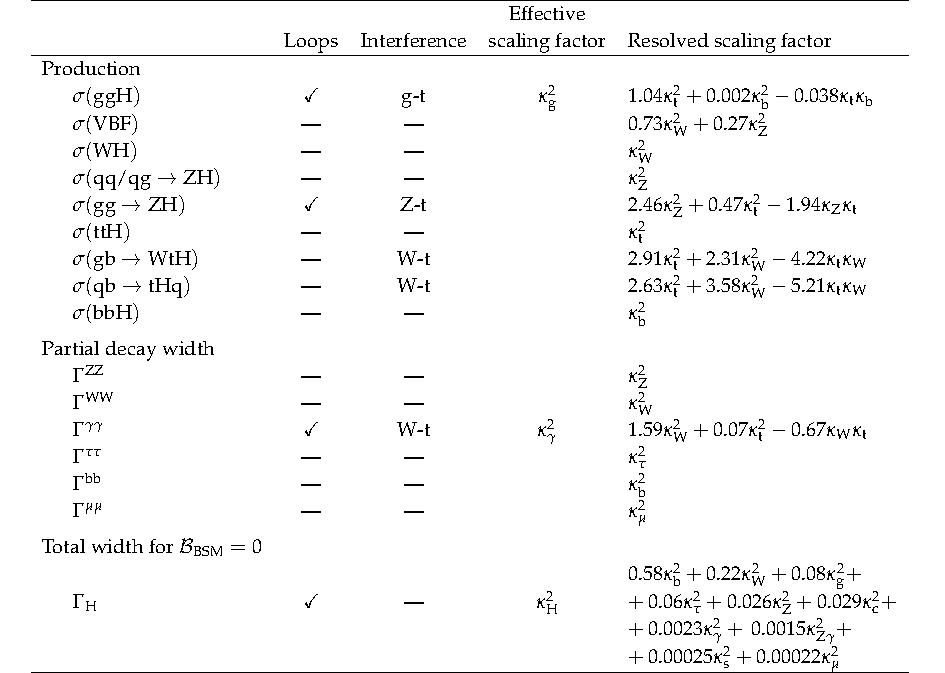
\includegraphics[width=1\textwidth]{Tables/hgg_results/kappa_table.pdf}
\end{table}

Using the notation introduced in section \ref{sec:category_likelihood}, the signal yields are parametrised as the product of scaling functions for each term in equation \ref{eq:kappa_param},

\begin{equation}
    \mu^{i,\gamma\gamma} = \frac{\sigma^i(\vec{\kappa})}{\sigma^i_{\rm{SM}}} \cdot \frac{\Gamma^{\gamma\gamma}(\vec{\kappa})}{\Gamma^{\gamma\gamma}_{\rm{SM}}} \cdot \frac{\Gamma_{\rm{H,SM}}}{\Gamma_{\rm{H}}(\vec{\kappa})}.
\end{equation}

\noindent
This approach works under the narrow Higgs boson width assumption, effectively factoring the total signal parametrisation into the effect at Higgs boson production and Higgs boson decay; a crucial concept in the EFT parametrisation discussed in the following chapter.

In this analysis two independent parametrisations are considered. The first uses the resolved scaling functions listed in Table~\ref{tab:kappa_param}, introducing universal coupling modifiers, $\kappa_V$ and $\kappa_F$, which modify the Higgs boson couplings to vector bosons and fermions, respectively, such that,
\begin{equation}
    \begin{split}
        % \centering
        \kappa_V = \kappa_W = \kappa_Z, \\
        \kappa_F = \kappa_t = \kappa_b = \kappa_\tau = \kappa_\mu. \\
    \end{split}
\end{equation}
\noindent
As shown in Table~\ref{tab:kappa_param}, the tHq and tHW production mode cross sections include an interference term proportional to the product, $\kappa_V\kappa_F$. This means that by measuring single-top associated production, the analysis gains sensitivity to the relative sign of the t-H (fermion) and V-H (vector boson) couplings, unlike when measuring ttH alone. Figure \ref{fig:kappa_F} shows both the observed (black) and expected (red) $q(\kappa_F)$ curves, where the value of $\kappa_V$ is profiled in the fit. In addition, the dashed red curve represents the expected likelihood that would be obtained if the tHq leptonic category is removed from the analysis. Clearly, the inclusion of the tHq leptonic category successfully reduces the degeneracy between positive and negative $\kappa_F$ values. The observed likelihood shows a slight favouring for negative $\kappa_F$ values with respect to the expected likelihood, due to the observed excess in the tH production cross section. Furthermore, the results of a two-dimensional likelihood scan in $\kappa_V$ and $\kappa_F$ are presented in the upper plot of Figure \ref{fig:2d_kappa}. The region with negative values of $\kappa_F$ is observed (expected) to be excluded with a significance of 0.5$\sigma$ (2.4$\sigma$).

\begin{figure}[htb!]
  \centering
  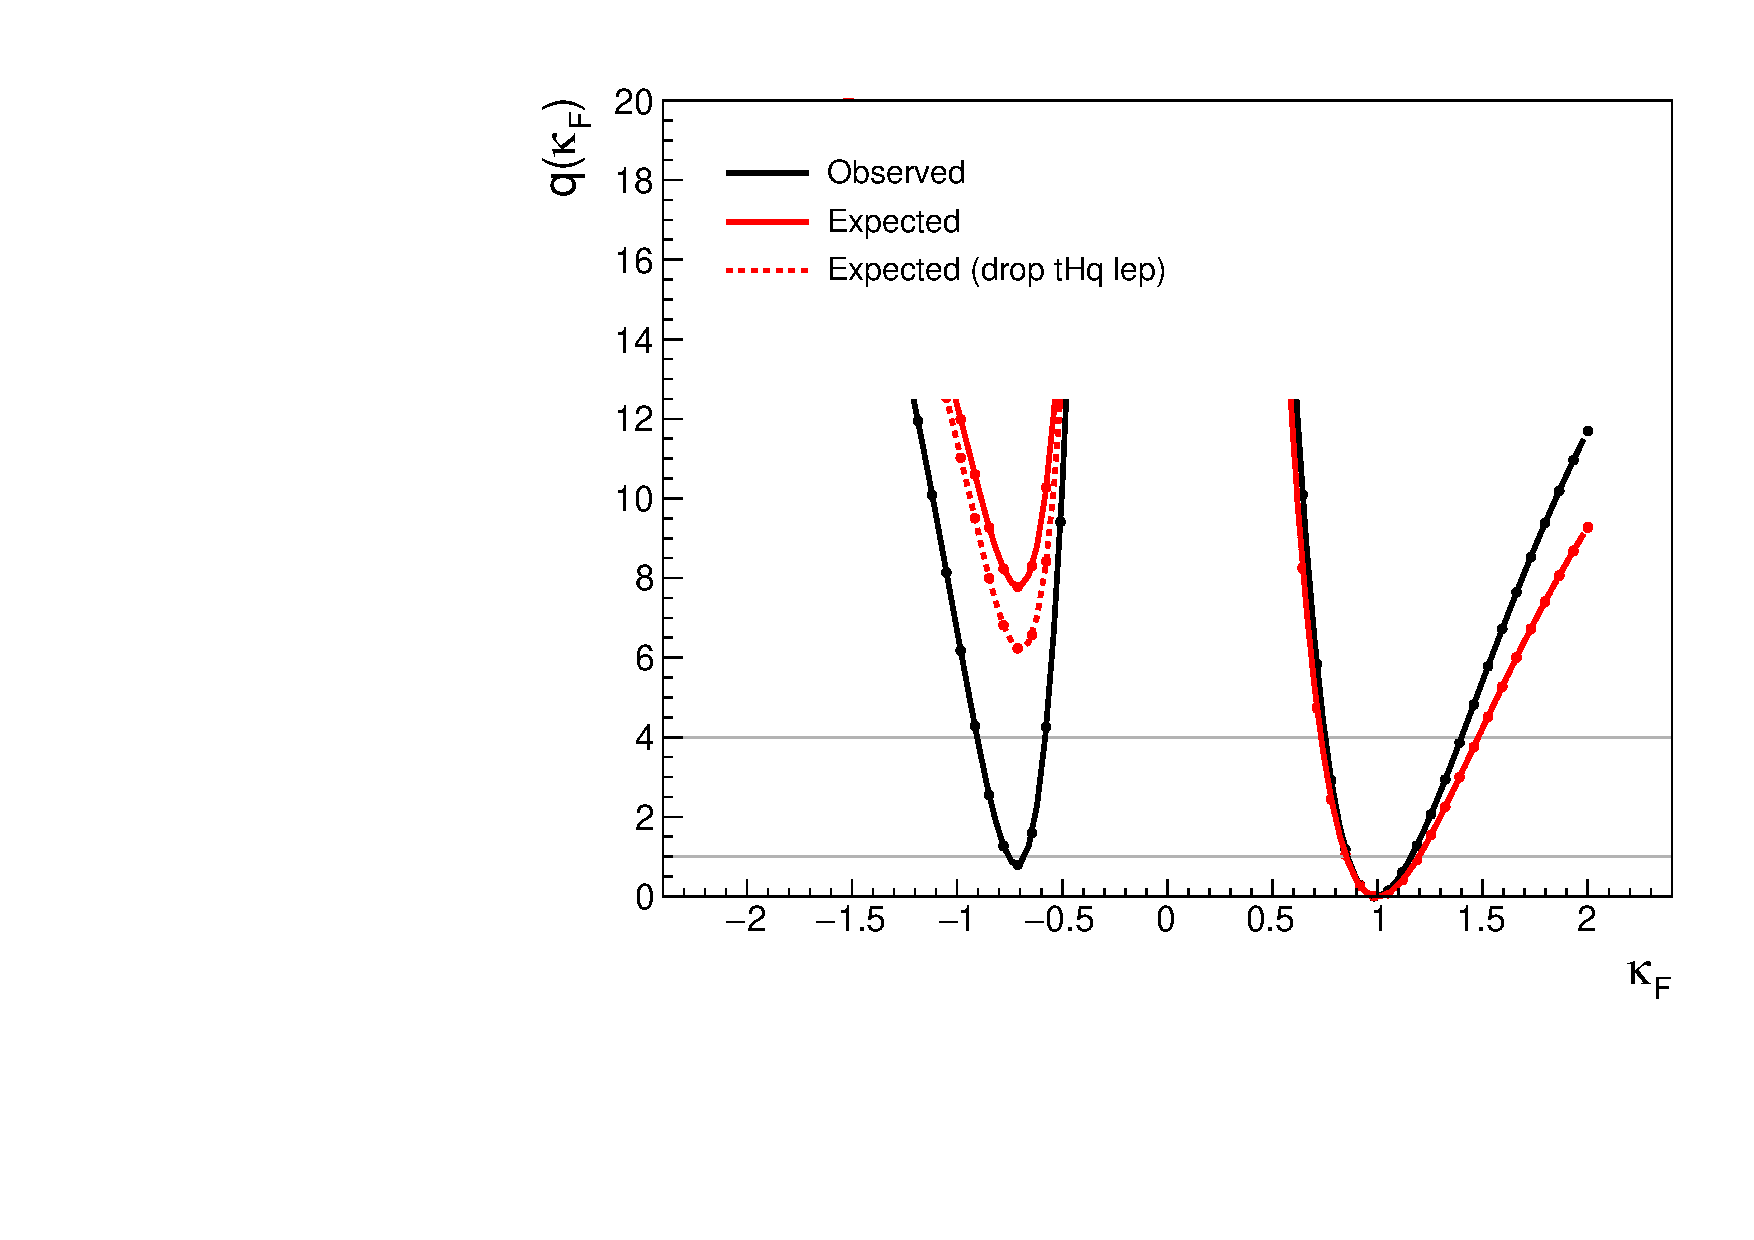
\includegraphics[width=.6\textwidth]{Figures/hgg_results/profile1D_kappa_F.pdf}
  \caption[Observed and expected likelihood curves for $\kappa_F$]
  {
    The observed (solid black) and expected (solid red) $q(\kappa_F)$ curves, where $\kappa_V$ is profiled in the fit. The expected curve that would be obtained by removing the tHq leptonic event category from the analysis is shown by the dashed red line.
  }
  \label{fig:kappa_F}
\end{figure}

The second parametrisation considered uses the effective coupling modifiers to gluons and photons, $\kappa_g$ and $\kappa_\gamma$, to measure potential deviations in the ggH and \Hgg loops. The observed results of a two dimensional likelihood scan in these two parameters is shown in the lower plot of Figure \ref{fig:2d_kappa}. In the scan, all other $\kappa$ parameters ($\kappa_t$,$\kappa_b$,$\kappa_W$,$\kappa_Z$,$\kappa_\tau$,$\kappa_\mu$) are fixed to unity. The $\kappa_g$ and $\kappa_\gamma$ parameters are particularly sensitive to additional heavy BSM particles, that would contribute to the rate of Higgs boson production and decay via loop processes. The observed best-fit point is consistent with the SM expectation at around the 68\% confidence level, suggesting there are no new states that add major contributions to the loops, or that the masses of any new states are significantly higher than the electroweak energy scale.

\begin{figure}[htb!]
  \centering
  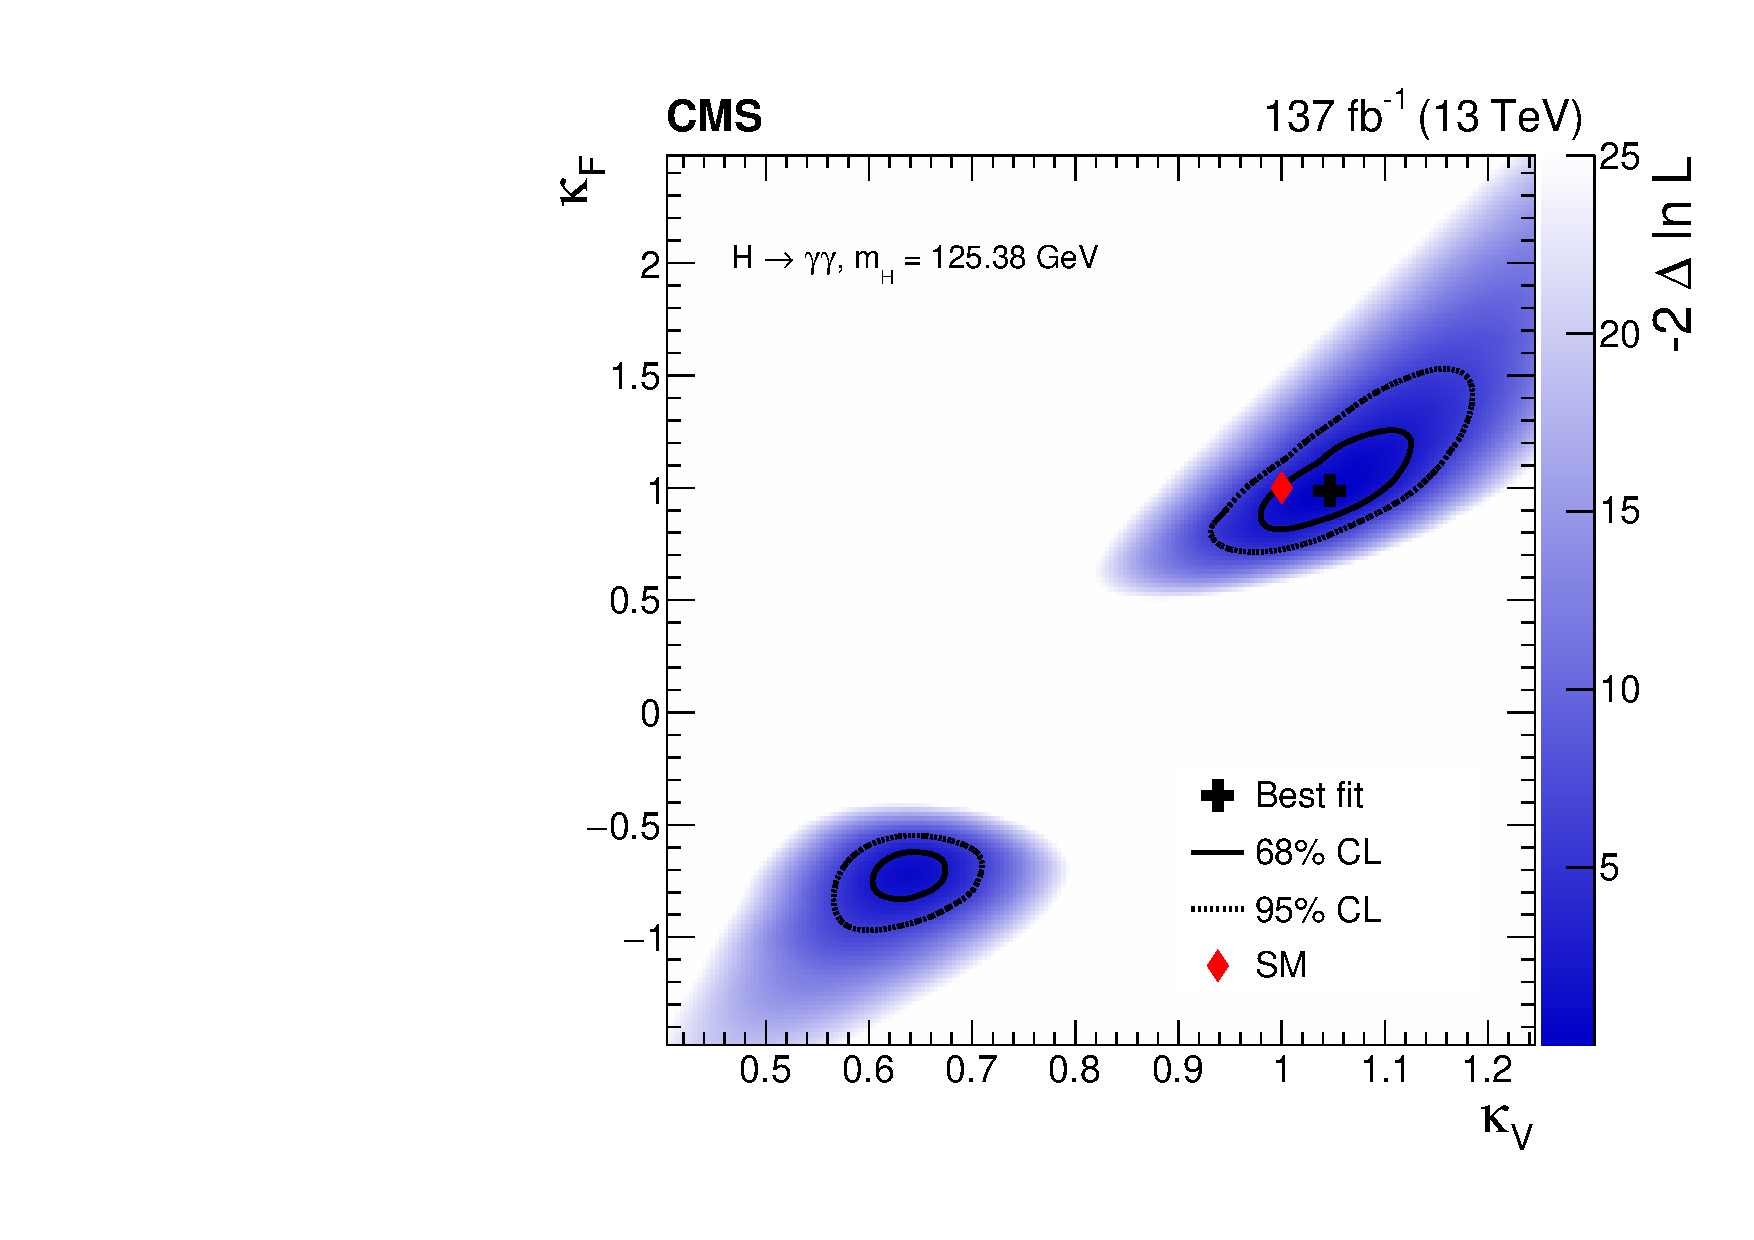
\includegraphics[width=.65\textwidth]{Figures/hgg_results/scan2D_kappa_V_vs_kappa_F_obs.pdf}
  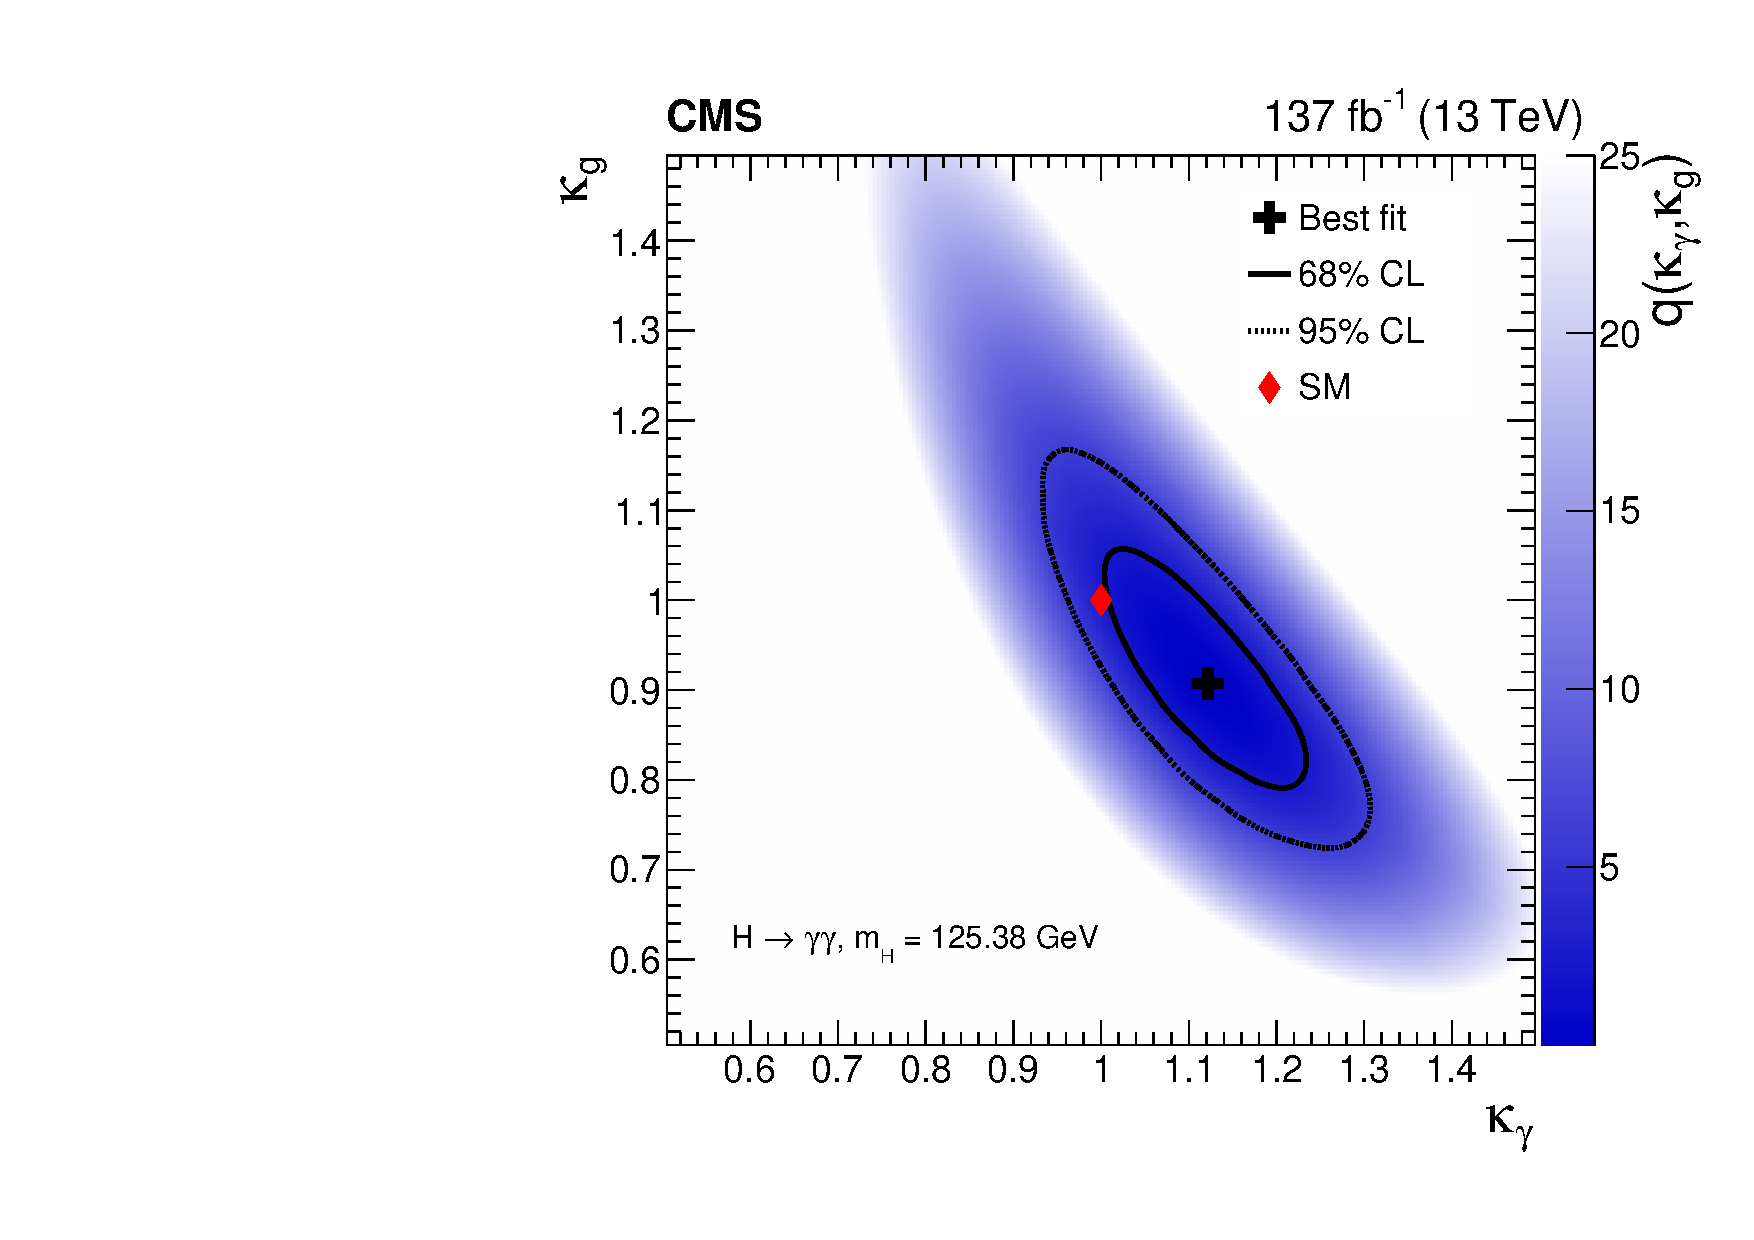
\includegraphics[width=.65\textwidth]{Figures/hgg_results/scan2D_kappa_gam_vs_kappa_g_obs.pdf}
  \caption[Two dimensional likelihood scans in the coupling modifier parametrisation]
  {
    Observed two dimensional likelihood scans performed in the $\kappa$-framework: $\kappa_V$ vs $\kappa_F$ using the resolved scaling functions (top), and $\kappa_\gamma$ vs $\kappa_g$ using the effective scaling functions (bottom). The 68\% and 95\% confidence level regions are represented by the solid and dashed contours, respectively. The best-fit and SM expected points are shown by the black cross and red diamond, respectively. The colour scale indicates the value of the test statistic, $q(\alpha_1,\alpha_2)$.
  }
  \label{fig:2d_kappa}
\end{figure}

Ultimately, the coupling modifier scaling functions are defined inclusively for each Higgs boson production mode cross section. As a result, this parametrisation does not make use of the kinematic information available in the STXS measurements. Introduced in the next chapter, the EFT parametrisation extends upon the $\kappa$-framework by defining scaling functions for each individual STXS bin. In this approach, the fit is able to use the kinematic information to more tightly constrain BSM physics.

\FloatBarrier

\section{Summary}
This section concludes the description of Higgs boson production cross section and couplings measurements using the diphoton decay channel. Chapter \ref{chap:hgg_overview} detailed the techniques used to reconstruct events consistent with the \Hgg decay in proton-proton collision data, and subsequently categorise them to become sensitive the different kinematic regions of the STXS framework. In chapter~\ref{chap:hgg_stats}, the statistical inference methods were described, which amount to performing a likelihood fit to the observed \mgg distribution in each analysis category. This chapter presented the results of the analysis which represent the most comprehensive study of Higgs boson production cross sections to date, using data collected by the CMS experiment.

A range of measurements are presented using different signal parametrisations. The inclusive Higgs boson signal strength is measured to be 1.12, relative to the SM prediction, with a $\pm 9\%$ uncertainty. This represents the most accurate measurement of this particular quantity in a single decay channel at CMS. A second fit is performed in the signal strength parametrisation, where the four principal Higgs boson production modes are scaled by a separate parameter. The simultaneous fit of these four signal strengths is found to be compatible with the SM prediction, with a $p$-value of 50\%. Moreover, each of the four production modes are now measured with uncertainties ranging from 10--35\%.

Production cross sections are measured in the STXS framework, using merging schemes of different granularities. In the maximal (minimal) merging scheme fit, a total of 17 (27) independent kinematic regions are measured simultaneously. The minimal merging scheme fit represents the most granular measurement of Higgs boson production performed in a single decay channel to-date. Both fits are compatible with SM predictions, with $p$-values of 31\% and 70\% for the maximal and minimal schemes, respectively. Many of the kinematic regions are measured here for the first time, including the measurement of ttH production in five different $p_T^H$ regions. Ultimately, by probing the different kinematic regions, we become sensitive to new physics which appears in specific regions of production phase space, hints of which would be washed out when measuring the equivalent processes inclusively. 

Furthermore, the measurement of ggH production with $\ptH>200$~GeV represents the most precise measurement of this particular kinematic region; a region which is sensitive to heavy BSM states appearing in the ggH loop. The cross section is found to be extremely compatible with the SM, with a measured value of $0.9^{+0.4}_{-0.3}$, relative to the SM prediction. Also, an upper limit is placed on the rate of tH production for the first time in the \Hgg decay channel at CMS. The observed (expected) limit at the 95\% C.L. is found to be 14 (8) times the SM prediction. All other results, including measurements of the Higgs boson coupling modifiers, are in agreement with the SM expectations.